\def\mode{1}
\if0\mode
\documentclass[journal,twoside,web]{ieeecolor}
\usepackage{generic}
\else
\documentclass[journal,twoside]{IEEEtran}
\fi
\usepackage[english]{babel}
\frenchspacing

% *** MISCELLANEA PACKAGES ***
%
\usepackage{microtype}
\usepackage{setspace}
\usepackage{blindtext}
\usepackage{siunitx}
\pagestyle{headings}
\usepackage{titlecaps}
\Addlcwords{or with if of and an to -off off for in into the versus vs subject} % excluded words
\usepackage{comment}

% *** GRAPHICS RELATED PACKAGES ***
%
\usepackage[caption=false]{subfig}
\captionsetup[subfigure]{font={scriptsize,sf}}
\usepackage{graphicx}
\usepackage{fancyhdr} 
\usepackage{color}
\usepackage{epsfig}
\graphicspath{{Images/}}
\usepackage{tikz}
\usetikzlibrary{patterns,fit,matrix}
\usepackage{tikzscale}
\usepackage{scalerel}
\usetikzlibrary{arrows}
\usetikzlibrary{plotmarks}
\usetikzlibrary{svg.path}
\usetikzlibrary{shapes.multipart}
\usepackage{pgfplots}
\usepgfplotslibrary{fillbetween}
\pgfplotsset{compat=newest}
\pgfplotsset{every axis/.append style={
		label style={font=\Large},
		tick label style={font=\large}  
}}
\tikzstyle{int}=[draw, fill=black!10, minimum size=5em,thick]
\tikzstyle{init} = [pin edge={to-,thick,black}]

% *** ALIGNMENT PACKAGES ***
%
\usepackage{array}
\usepackage{stfloats}

% *** MATH PACKAGES ***
%
\let\proof\relax \let\endproof\relax
\usepackage{amsmath,amssymb,amsfonts,amsthm}
\numberwithin{equation}{section}
\usepackage{mathdots}
\usepackage{bbm,dsfont}
\usepackage{relsize}
\usepackage{nicefrac}
\usepackage{bbm}
\usepackage{mathtools}
\usepackage[mathscr]{eucal}

% *** SPECIALIZED LIST PACKAGES ***
%
\usepackage[ruled]{algorithm}
\usepackage{algpseudocode}
\usepackage{multirow}
\usepackage{makecell}
\makeatletter
\gdef\Shortstack{\@ifnextchar[\@Shortstack{\@Shortstack[c]}}
\gdef\@Shortstack[#1]#2{%
	\leavevmode
	\vbox\bgroup
	\baselineskip-\p@\lineskip 3\p@
	\let\mb@l\hss\let\mb@r\hss
	\expandafter\let\csname mb@#1\endcsname\relax
	\let\\\@stackcr\setlength{\baselineskip}{#2}%
	\@ishortstack}
\makeatother
\usepackage{booktabs}
\usepackage{tabularx}
\let\labelindent\relax
\usepackage{enumitem}

% *** FLOAT PACKAGES ***
%
\usepackage{float}
\usepackage[absolute]{textpos}

% *** PDF, URL AND HYPERLINK PACKAGES ***
%
\usepackage{url}
\usepackage{hyperref}
\makeatletter
\let\NAT@parse\undefined
\makeatother
\usepackage[capitalize]{cleveref}
\pdfminorversion=4

% *** CITATION PACKAGES ***
%
\usepackage{cite}

% link to ORCID
\newcommand\orcidicon[1]{\href{https://orcid.org/#1}{\includegraphics[scale=0.04]{orcid.pdf}}}

% correct bad hyphenation here
\hyphenation{op-tical net-works semi-conduc-tor}

% personalized commands
%!TEX root = ../book.tex
%%%%
%% section and chapter symbol
\newcommand{\secn}{\S}
\newcommand{\chp}{\S}

%%%% 
%% my environment for assumptions%%%
%%%%

\newenvironment{myassumptions}{%
   \begin{description}[style=multiline, leftmargin = 18pt, align=left]%
}{%
   \end{description}%
}
%%%%%
%%%%

%% ENUMERATED LABEL FOR ASSUMPTIONS
\makeatletter
\def\nl#1#2{\begingroup
    #2%
    \def\@currentlabel{#2}%
    \phantomsection\label{#1}\endgroup
}
\makeatother
%%%%%%
%%%%
%%

% to box multiple equations

\newenvironment{boxalign}[1]% 
{\ensuremath{
\begin{empheq}[box=\fbox]{align}
{#1}
\end{empheq}
}}


\newenvironment{advanced}{\small\fontfamily{ppl}\selectfont}{}
% ----- theorem-like environments                                                                                                   
\newtheorem{theorem}            {Theorem}[section]
\newtheorem{conjecture}            {Conjecture}[section]
\newtheorem{corollary}          [theorem]{Corollary}
\newtheorem{proposition}        [theorem]{Proposition}
\newtheorem{definition}         [theorem]{Definition}
\newtheorem{example}            [theorem]{Example}
\newtheorem{lemma}              [theorem]{Lemma}
\newtheorem{ass}                [theorem]{Assumption}
\newtheorem{remark}             [theorem]{Remark}
\newtheorem{result}             [theorem]{Result}



\newcommand{\normal}{\mathbfit{N}}  % this is the distribution
\newcommand{\uniform}{u}  % this is the rv

\newenvironment{boxresult}[1]% 
{
\begin{mdframed}
\par\noindent\textbf{#1:}\begin{rmfamily}\noindent}% 
{\end{rmfamily}
\end{mdframed}
} 

\newcommand{\pwe}{Complements and Sources}

%\newcommand{\Ep}{\E_\pdf}
\newcommand{\Ept}{\E_{\beliefm_\infty}}

\newcommand{\I}{\Pi}
\newcommand{\avg}{\phi}
\newcommand{\unavg}{L}
\newcommand{\dob}{\rho}  %dobrushin
\newcommand{\dist}{D}
\newcommand{\bias}{\operatorname{Bias}}
\newcommand{\var}{\operatorname{Var}}
\newcommand{\msd}{\operatorname{MSD}}

% prob, expectation

\newcommand{\rv}{x}
\newcommand{\rvY}{y}
\newcommand{\cdfb}{\bar{\cdf}}
\newcommand{\outcome}{\zeta}
\newcommand{\pdfX}{p}
\newcommand{\pdfY}{q}

\newcommand{\pdf}{p}
\newcommand{\cdf}{F}
\newcommand{\prob}{\mathbb{P}}
\newcommand{\E}                 {\Bbb{E}}
\newcommand{\bE}{\bar{\E}}
\renewcommand{\P}                 {\Bbb{P}}
\newcommand{\cov}{\operatorname{cov}}
\newcommand{\bre}{\mathbf{L}}
\newcommand{\pref}{q}  % reference prob method  density under \bar{P}

% state space
\newcommand{\grid}{\state}
\newcommand{\lowdim}{r}
\newcommand{\inp}{u}
\newcommand{\bstate}{\bar{\state}}
\newcommand{\onoisevar}{\sigma^2_\onoise}

\newcommand{\borelset}{S}
\newcommand{\tstate}{\tilde{\state}}

\newcommand{\obs}{y}
%\newcommand{\Obs}{\mathbf{y}}
\newcommand{\Obs}{\obs}

\newcommand{\snoise}{w}
\newcommand{\onoise}{v}
\newcommand{\statem}{A}
%\newcommand{\statem}{F}

\newcommand{\statemg}{\phi}
\newcommand{\obsmg}{\psi}
\newcommand{\snoisem}{\Gamma}

\newcommand{\obsm}{C}
%\newcommand{\obsm}{H}

%\newcommand{\obsmnew}{\psi}
\newcommand{\obsmnew}{H}
\newcommand{\level}{g}

%\newcommand{\onoisem}{D}
\newcommand{\onoisem}{D}
\newcommand{\inpm}{f}
\newcommand{\oinpm}{g}
\newcommand{\snoisecov}{Q}
\newcommand{\onoisecov}{R}
\newcommand{\onoisecovnew}{R}
\newcommand{\ar}{a} % AR coefficients
\newcommand{\arp}{s} % ar process

\newcommand{\state}{x}
\newcommand{\statespace}{\mathcal{X}}
\newcommand{\obspace}{\mathcal{Y}}
\newcommand{\statedim}{X}
\newcommand{\obsdim}{{Y}}

\newcommand{\mc}{r}  % markov chain of JMLS
\newcommand{\finals}{x} % reciprocal markov process

\newcommand{\fun}{\phi}
\newcommand{\funbar}{\psi}

\newcommand{\obsdummy}{y}

\newcommand{\identity}{I}



%% stoch convergence
\newcommand{\law}{\stackrel{\mathcal{L}}{=}}

% VARIATIONAL DISTANCE
\newcommand{\dvar}[2]{\|{#1}-{#2}\|_{\text{\tiny{TV}}}}
\newcommand{\dvarsq}[2]{\|{#1}-{#2}\|^2_{\text{\tiny{TV}}}}
\newcommand{\dvarn}{\| \cdot \|_{\text{\tiny{TV}}}}

% HMM parameters
\newcommand{\oprob}{B}
\newcommand{\tp}{P}
\newcommand{\utp}{\bar{\tp}}
\newcommand{\ltp}{\underline{\tp}}


\newcommand{\btp}{\bar{\tp}}
\newcommand{\jump}{J}
\newcommand{\duration}{D}
\newcommand{\sensm}{S^\model}

\newcommand{\eigenvec}{\nu}
%%

\newcommand{\finaltime}{N}
\newcommand{\btime}{\finaltime}


% models
\newcommand{\model}{\theta}
\newcommand{\modelpsi}{\psi}
\newcommand{\truemodel}{\model^o}
\newcommand{\modelem}{\model_\text{EM}}
\newcommand{\modelnr}{\model_\text{NR}}

\newcommand{\Model}{\Theta}
\newcommand{\lik}{L_\finaltime} % likelihood
\newcommand{\logl}{\mathcal{L}_\finaltime}  % log likeilhood
\newcommand{\aux}{\mathcal{Q}}  % EM algorithm Q aux likelihood

\newcommand{\beliefm}{\belief_\model}
\newcommand{\Mbelief}{\Pi_\infty}


\newcommand{\ubeliefm}{\ubelief^\model}
\newcommand{\likc}{\pdf(\obs_{1:\finaltime}| \model)}
\newcommand{\pdfm}{\pdf^\model}
\newcommand{\mle}{\model^*}
\newcommand{\ml}[1]{{#1}^*}
\newcommand{\oprobm}{\oprob^\model}
\newcommand{\tpm}{{\tp_\model}}
\newcommand{\nablam}{\nabla_\model}
\newcommand{\ardim}{M} % dimension of ar model
\newcommand{\sigmasnoise}{\sigma}

% radar
\newcommand{\range}{d}

% belief space
\newcommand{\belief}{\pi}
\newcommand{\beliefzero}{\belief}
\newcommand{\bbelief}{\bar{\pi}}
\newcommand{\ubelief}{{q}}
\newcommand{\upbelief}{\bar{\pi}}
\newcommand{\lbelief}{\underline{\pi}}

\newcommand{\lmean}{\underline{\state}}
\newcommand{\mean}{{\hat{\state}}}
\newcommand{\umean}{\bar{\state}}


\newcommand{\mat}{M}
\newcommand{\diff}{L^\epsilon}

%%%%%%%%%%

\newcommand{\Belief}{\Pi(\statedim)}
\newcommand{\back}{\beta}
\newcommand{\bay}[2]{\mathcal{B}[{#1},{#2}]}
\newcommand{\diagp}{P}


%social learning
\newcommand{\tbelief}{\pi^0}
\newcommand{\history}{\mathcal{H}}
\newcommand{\full}{\mathcal{F}}

\newcommand{\sigs}{\sigma}
\newcommand{\Bs}{R^\pi} 
\newcommand{\Bsl}{R^n}
\newcommand{\priv}{\eta}
\newcommand{\etaregion}{\kappa}

   \newcommand{\ca}{\cost_\action}
   \newcommand{\socialcost}{l}
   \newcommand{\ta}{\tilde{\action}}
   \newcommand{\sA}{\mathcal{A}}
   
   % incest 
   \newcommand{\quantized}{Q}
   
% Kalman filter variables
\newcommand{\kalmancov}{\Sigma}
\newcommand{\kalmangain}{K}
\newcommand{\lqgain}{L}
\newcommand{\kgain}{\bar{K}}  % this satisfies A L = kalmangain
\newcommand{\tr}{\normalfont{\text{trace}}}
\newcommand{\Sig}{S}   %  used for S_k in Kalman filter
\newcommand{\prederr}{\nu}
\newcommand{\ksgain}{G}

% delay variables
\newcommand{\delay}{\Delta}
\newcommand{\Delay}{\Delta}
\newcommand{\delaydim}{L}
\newcommand{\tpd}{\tp^{(\delay)}}
\newcommand{\dobs}{z}



\newcommand{\delaysetim}{\{1,2,\ldots,L-1\}}
\newcommand{\Delayset}{\{0 \text{ (announce change)} ,\D_1,\D_2,\ldots,\D_L\}}
\newcommand{\Delayseti}{\{0 \text{ (announce change)} ,1,2,\ldots, L\}}


% particle filter
\newcommand{\imp }{\pi}
\newcommand{\weight}{\omega}
\newcommand{\nw}{\tilde{\weight}}  % particle filter normalized weight
\newcommand{\ole}{\stackrel{\text{defn}}{=}}


% additive functional
\newcommand{\af}{S}  % ADDITIVE functional
\newcommand{\mf}{\mu}   % measure valued pdf of functional


\newcommand{\est}{\kappa}
\newcommand{\Est}{\boldsymbol{\kappa}}

\newcommand{\gtp}{\underset{\text{\tiny TP2}}{\geq}}
\newcommand{\gr}{\geq_r}
\newcommand{\lr}{\leq_r}
\newcommand{\gs}{\geq_s}
\newcommand{\ls}{\leq_s}






\newcommand{\filterd}{\sigma}
\newcommand{\filtern}{\alpha}
\newcommand{\filternum}{\gamma}
\newcommand{\filter}{T}
\newcommand{\bayes}{\mathcal{B}}

\renewcommand{\vec}{\operatorname{vec}}

\newcommand{\argmin}{\operatornamewithlimits{argmin}}
\newcommand{\argmax}{\operatornamewithlimits{argmax}}

\newcommand{\reals}{{\rm I\hspace{-.07cm}R}}
\newcommand{\R}{{\rm I\hspace{-.07cm}R}}
\newcommand{\N}{{\rm I\hspace{-.07cm}N}}
\newcommand{\continuous}{{\rm I\hspace{-.16cm}C}}

\newcommand{\F}{\mathcal{F}}   % sigma algebra

\newcommand{\beq}{\begin{equation}}
\newcommand{\eeq}{\end{equation}}
\newcommand{\nn}{\nonumber}

\renewcommand{\(}		{\left(}
\renewcommand{\)}		{\right)}


\newcommand{\Y}{\mathbf{Y}}

\renewcommand{\th}{\theta}
\newcommand{\Th}{\Theta}

\newcommand{\p}{\prime}

\newcommand{\one}{\mathbf{1}}
\newcommand{\ones}{\mathbf{1}}
\newcommand{\zero}{\mathbf{0}}


% tracking variables
\newcommand{\pos}{p}
\newcommand{\samt}{\Delta}
\newcommand{\jerk}{q}
\newcommand{\assoc}{a}

\newcommand{\f}{f} % false measurement

%%%%% continuous time


\newcommand{\bs}{\bar{\sigma}}
\newcommand{\osig}{\mathcal{Y}}
\renewcommand{\div} {{\operatorname{div}}}
\newcommand{\ftime}{T}
\newcommand{\gen}{Q}
\newcommand{\diag}{\textnormal{diag}}

\newcommand{\bop}{\mathcal L}
\newcommand{\fop}{\bop^*}

\newcommand{\pnoise}{\nu}
\newcommand{\rate}{\lambda}
\newcommand{\pois}{N}
\newcommand{\markpdf}{\pdf}
\newcommand{\marked}{z}
\newcommand{\event}{t}
\newcommand{\markspace}{\mathcal M}
\newcommand{\sigf}{\mathcal{F}}
\newcommand{\testf}{\phi}
\newcommand{\mart}{M}

\newcommand{\bq}{\bar{\ubelief}}
\newcommand{\be}{\bar{\epsilon}}
\newcommand{\bback}{\bar{\back}}

\newcommand{\forwardzakai}{q}
\def\la{\langle}
\def\ra{\rangle}


%structural filter
\newcommand{\gRm}{\succeq_M}
\newcommand{\lRm}{\preceq_M}
\newcommand{\uA}{\underline{A}}

\renewcommand{\i}{\mathbf{i}}
\renewcommand{\j}{\mathbf{j}}
\newcommand{\gtptwo}{\underset{\text{\tiny TP2}}{\geq}}
\newcommand{\ltptwo}{\underset{\text{\tiny TP2}}{\leq}}

\newcommand{\nm}{L}
\newcommand{\lR}{\preceq}
\newcommand{\gR}{\succeq}
\newcommand{\cons}{{\text{\bf Cons}}}
\newcommand{\consb}{\overline{\text{\bf Cons}}}
\newcommand{\conv}{{\text{conv}}}

\newcommand{\levels}{g}

\newcommand{\map}{\hat{\state}^{\text{MAP}}}
\newcommand{\lmap}{\underline{\state}^{\text{MAP}}}
\newcommand{\umap}{\bar{\state}^{\text{MAP}}}


% STOCHASTIC CONTROL
\newcommand{\Minimize}{\operatorname{Minimize}}
\newcommand{\marginal}{p}
\newcommand{\bmodel}{\bar{\model}}
\newcommand{\hQ}{\hat{Q}}

\newcommand{\ltwo}{\log_2}

%\newcommand {\brMet}{\ensuremath{\rho}} % the metric on the space \brSpc 
\newcommand{\sgain}{M}
\newcommand{\again}{N}
\newcommand{\fgain}{L}

\newcommand{\terminalcosta}{\cost_{\finaltime+1}}
\newcommand{\actions}{\action^\state}
\newcommand{\actionm}{\action^\obs}

\newcommand{\dpop}{L}
\newcommand{\cost}{c}
\newcommand{\covcost}{C}
\newcommand{\reward}{r}
\newcommand{\terminalcost}{\cost_\finaltime}
\newcommand{\Cost}{C}
\newcommand{\nlcost}{d}
\newcommand{\nlCost}{D}

\newcommand{\yi}{y^{(1)}}
\newcommand{\yii}{y^{(2)}}
\newcommand{\valueft}{\tilde{\valuef}}

\newcommand{\bmc}{\bar{m}}

\newcommand{\bQ}{\bar{Q}}
\newcommand{\bvalueb}{\bar{\valueb}}

\newcommand{\action}{u}
\newcommand{\baction}{\bar{\action}}
\newcommand{\actionspace}{\,\mathcal{U}}
\newcommand{\actiondim}{U}
\newcommand{\laspace}{\mathcal{A}}
%\newcommand{\cost}{c}
\newcommand{\totalcost}{J}
\newcommand{\exptotalcost}{J_{\bpolicy}}
\newcommand{\opttotalcost}{J_{\bpolicy^*}}
\newcommand{\discount}{\rho}

\newcommand{\region}{\mathcal{R}}
\def \con {{\beta}}
\def \rcon {{\gamma}}
\def \Con {{B}}
\def\param{{\alpha}}
\def \Z {{\cal Z}}
%%%% \def \a {{\alpha}}
\def \a {{\psi}}
\def\Param{{\boldsymbol{\alpha}}}
\def \Epi {{\E}_{\pi(\param)}}
 \def \G{{B}}
 \newcommand{\statpi}{\pi}
 \newcommand{\Ep}{\E_{\policy}}

\def\Policy{{\boldsymbol{\policy}}}
\newcommand{\policy}{\mu}
\newcommand{\optpolicyv}{\bpolicy^*}
\newcommand{\optpolicy}{\policy^*}
\newcommand{\bpolicy}{{\boldsymbol{\mu}}}
\newcommand{\optimaltotalcost}{J_{\optpolicy}}
\newcommand{\valuef}{V}
\newcommand{\valuefb}{\bar{\valuef}}
\newcommand{\valueb}{J}
\newcommand{\info}{\mathcal{I}}
\newcommand{\uV}{\underline{V}}

\newcommand{\bvalvec}{\bar{\gamma}}
\newcommand{\valvec}{\gamma}
\newcommand{\Valvec}{\Gamma}

\newcommand{\overlook}{\beta}
\newcommand{\blockprob}{q}
\newcommand{\augss}{\bar{\statespace}}
\newcommand{\terminal}{T}
\newcommand{\schRwd}{h}
\newcommand{\actionCost}{\cost}
\newcommand{\schHst}{\info}
\newcommand{\policySpc}{\mathcal{U}}
\newcommand{\schRwdFn}{J}

% stopping set
\newcommand{\stopset}{\mathcal{S}}

% POMDP (pom) quantities

\newcommand{\Jh}{J^{\text{h}}}
\newcommand{\Jo}{\bar{J}}
\newcommand{\thstate}{\state}
\newcommand{\thstatedim}{\statedim}

\newcommand{\pie}{\pi^{\epsilon_1,\epsilon_2,\ldots,\epsilon_{\statedim-1}}}
\newcommand{\pieone}{\pi^{\epsilon_1,\ldots\epsilon_j,\ldots, \epsilon_{\statedim-1}}}
\newcommand{\pietwo}{\pi^{\epsilon_1,\ldots\bar{\epsilon}_j,\ldots, \epsilon_{\statedim-1}}}


\newcommand{\Pimon}{\Pi_{\mathcal{M}}}
\newcommand{\beliefmon}{\belief_{\mathcal{M}}}

\newcommand{\ric}{\Gamma}
\newcommand{\iter}{n}
\newcommand{\iterfinal}{N}

\renewcommand{\time}{k}
\newcommand{\timet}{t}


\newcommand{\Hyperplane}{\mathcal{H}}


\newcommand{\Io}{{\Pi^o(X)}}
\newcommand{\Ib}{{\Pi^b(X)}}


\newcommand{\poly} {S}

\renewcommand{\l}{\mathcal{L}}


\newcommand{\unordered}{\sim}

\newcommand{\eye}{\textit{I}}
\newcommand{\bd}{\succeq_{\mathcal{B}}}
\newcommand{\aB}{R}
\newcommand{\tpone}{{\tp}}
\newcommand{\tptwo}{\bar{\tp}}

\newcommand{\tpe}{p}
\newcommand{\oprobe}{b}
\newcommand{\boprob}{\bar{\oprob}}

\newcommand{\noise}{n}
\newcommand{\asmp}{\textbf{A}}
\newcommand{\asmpg}{\bar{\text{A}}}

\newcommand{\statelvl} {h}
\newcommand{\sqg} {H}
\newcommand{\expcost} {C}

\newcommand{\cop}{C_o}
\newcommand{\thr}{\mathbf{\Gamma}}
\newcommand{\copomat}{\Gamma}

\newcommand{\uvalue}{\underline{V}}
\newcommand{\bvalue}{\overline{V}}
\newcommand{\valueaction}{Q}
\newcommand{\uvalueaction}{\underline{Q}}
\newcommand{\bvalueaction}{\overline{Q}}
\newcommand{\optvalue}{V}
\newcommand{\trid}{\Upsilon}
\newcommand{\filternorm}{\sigma}

\newcommand{\gc} {\succeq}
\newcommand{\lc} {\preceq}

%\newcommand{\ls}{_{s}{\le}}
\newcommand{\error}  {\eta}


\newcommand{\mus}{{\mu^*(\model)}}
\newcommand{\bmus}{{\mu^*(\bmodel)}}

\newcommand{\tcost}[1]{J_\mu^{(#1)}}


\newcommand{\rmm}{\rho_{\model,\bmodel}}

\newcommand{\lcost}{\underline{\textit{C}}}
\newcommand{\ucost}{\overline{\textit{C}}}
\newcommand {\uf} {\textit{f}}%{\underline{\textit{f}}\xspace}
\newcommand {\of} {\textit{g}}%{\overline{\textit{f}}\xspace}
\newcommand {\nooverlap} {\bar{\Belief}}
\newcommand {\setoverlap} {{\Pi_{O}}}
%\newcommand {\optpolicy} {\mu^*}
\newcommand {\policyu} {\overline{\mu}}
\newcommand {\policyl} {\underline{\mu}}


\newcommand{\yp}{y_{\pi;\model}^*}
\newcommand{\yps}{y_{\pi;\model,\bmodel}^*}
\newcommand{\ypsx}{y_{e_X;\model,\bmodel}^*}
\newcommand{\ytt}{y^*_{\model,\bmodel}}


\newcommand {\Timel} {\Gamma_l}
\newcommand {\Timev} {\Gamma_v}
%\newtheorem{mytheorem}{Theorem}
%\newcommand{\argmin}{\operatornamewithlimits{argmin}}
\newcommand{\basisvec} {\textit{e}}
\newcommand {\vect} {\textit{v}}
\newcommand {\percentloss} {\epsilon}
\newcommand {\approxpolicy} {\tilde{\mu}}
\newcommand{\bT}{\bar{T}}
\newcommand{\bsigma}{\bar{\sigma}}
\newcommand{\pomSt}{\ensuremath{s}}
\newcommand{\pomStSpc}{\ensuremath{S}}
\newcommand{\pomRwd}{\ensuremath{g}}
\newcommand{\pomTranMat}{\ensuremath{P}}
\newcommand{\pomObsMat}{\ensuremath{R}}
\newcommand{\pomAct}{\ensuremath{a}}
\newcommand{\pomActSpc}{\ensuremath{A}}
\newcommand{\pomObs}{\ensuremath{\theta}}
\newcommand{\pomObsSpc}{\ensuremath{\Theta}}
\newcommand{\pomHst}{\ensuremath{\Psi}}
\newcommand{\pomPol}{\ensuremath{\delta}}
\newcommand{\pomPolSpc}{\ensuremath{\Delta}}
\newcommand{\pomRwdFn}{\ensuremath{V}}
\newcommand{\pomHMM}{\ensuremath{\Phi}}
\newcommand{\pomPolVecSet}{\ensuremath{\Gamma}} % the PWLC representation of a policy
\newcommand{\pomPolVec}{\ensuremath{\gamma}}
\newcommand{\pomPolMapLB}{\ensuremath{\underline{\cal{H}}}} % lovejoy lower bound
\newcommand{\pomPolMapUB}{\ensuremath{\overline{\cal{H}}}} % lovejoy upper bound
\newcommand{\pomPolMap}{\ensuremath{\mathcal{H}}}

\newcommand{\comAct}{\pomAct} %
\newcommand{\comActSpc}{\pomActSpc}
\newcommand{\comObs}{\pomObs}
\newcommand{\comObsSpc}{\pomObsSpc}
\newcommand{\comPol}{\pomPol}
\newcommand{\comPolSpc}{\pomPolSpc}
\newcommand{\comRwdFn}{\pomRwdFn}
\newcommand{\obsMat}{R}



\newcommand{\gl}{\geq_{L_i}}
\newcommand{\glp}{\geq_{L_{i+1}}}

\newcommand{\glx}{\geq_{L_x}}
\newcommand{\glX}{\geq_{L_X}}
\newcommand{\glone}{\geq_{L_1}}


\newcommand{\bp}{{\bar{\pi}}}
%%
%grad
\def \La {{\cal L}}
\def \GF{{\widehat{\nabla C}^{\text{WD}}}}
\def \GS{{\widehat{\nabla C}^{\text{Score}}}}


%% SPSA
\newcommand{\wderiv}{g}
%\newcommand{\deriv}{L}
\newcommand{\hphi}{\hat{\phi}}
\newcommand{\nablat}{\widehat{\nabla}_{\phi}}
\newcommand{\direction}{\omega}

%%%%
%Sensor scheduling
\newcommand{\ac}{\tt{active}}
\newcommand{\co}{\tt passive}
\newcommand{\pr}{\tt predict}
\newcommand{\fa}{\rho^{\text{\ac}}}
\newcommand{\fc}{\rho^{\text{\co}}}
\newcommand{\fp}{\rho^{\text{\pr}}}
\newcommand{\ha}{r^{\text{\ac}}}
\newcommand{\hc}{r^{\text{\co}}}
\newcommand{\hp}{r^{\text{\pr}}}
\newcommand{\use}{n}
\newcommand{\tar}{z}

%%% quickest detection
%%%%%%
\newcommand{\epoch}{\tau}
\newcommand{\D}{D}
\newcommand{\delayset}{\{\D_1,\D_2,\ldots,\D_L\}}
\newcommand{\delayseti}{\{1,2,\ldots,L\}}
\newcommand{\kstar}{k^*}
\newcommand{\changetime}{\tau^0}
\newcommand{\falsealarm}{{f}}
\newcommand{\Vb}{\bar{V}}
\newcommand{\Pp}{\P_\mu}
\newcommand{\Cb}{\bar{C}}
\newcommand{\risk}{\epsilon}
%%%%
\newcommand{\stepsize}{\epsilon}

\newcommand{\A}{\mathbb{A}}
%%%%

%%%radar
\newcommand{\bkalmancov}{\bar{\Sigma}}
\newcommand{\price}{\nu} %{\mathbf{\nu}}
\newcommand{\Mu}{\boldsymbol{\mu}}
\newcommand{\grnew}{\succeq}
\newcommand{\gsnew}{\succ}
\newcommand{\lrnew}{\preceq}
\newcommand{\Q}{\mathcal{Q}}
\newcommand{\bt}{\underline{\theta}}
\newcommand{\lstar}{{l^*}}
\def\Lyapunov{{\cal L}}
\def\Ricatti{{\cal R}}
\def\pdfmat{\mathcal{M}}
%%%
%bandit
\newcommand{\numtarget}{L}
\newcommand{\target}{l}
\newcommand{\delt}{\delta}

%%%%%%%%

%%% disc opt %%
\newcommand{\bm}{w}
\newcommand{\globalopt}{\mathcal{G}}
\newcommand{\cd}{(\cdot)}
%\newcommand{\br}{\boldsymbol{b}^{\gamma}}
\newcommand{\br}{{b}^{\gamma}}
\newcommand{\bbr}{b^{\gamma}}
\newcommand{\boldf}{f}
\def\z{\mathbf{z}}
\def\lb{\left[}
\def\rb{\right]}
\def\lbr{\left\lbrace}
\def\rbr{\right\rbrace}
\def\RR{{\mathbb{R}}}
\newcommand{\pp}{{\mathbb P}}
\newcommand{\maxdiff}{D}

\newcommand{\score}{S}
\newcommand{\batchsize}{N}
\newcommand{\infodelta}{\info^\Delta}

%\newcommand{\degreelink}{\alpha}
\newcommand{\degreelink}{\th}
%%%%

%%%
%% primal dual
%%

\newcommand{\penaltyweight}{\Delta}

%%%%%
%%
%%% part 4  commands  %%%
%%%%
\def\ph{\varphi}
\newcommand{\M}{{\cal M}}
\newcommand{\lbar}{\overline}
\newcommand{\wdt}{\widetilde}

%\def\l{\Big|}

%\def\r{\Big|}
\newcommand{\ad}{&\!\!\!\disp}
\newcommand{\aad}{&\disp}
\newcommand{\barray}{\begin{array}{ll}}
\newcommand{\earray}{\end{array}}
\newcommand{\disp}{\displaystyle}

\newcommand{\h}{{\ell}}
\def\cd{(\cdot)}
\newcommand{\e}{\varepsilon}
\newcommand{\tth}{\tilde{\th}}
%%%
%%%
%% population dynamics and social network
\newcommand{\numagents}{M}

\newcommand{\nature}{\state}
\newcommand{\pop}{\theta}
\newcommand{\bpop}{\bar{\pop}}
\newcommand{\mpop}{\bar{\pop}}
\newcommand{\popspace}{\Theta}
\newcommand{\pa}{\alpha}

\newcommand{\network}{G}
\newcommand{\Vertexset}{V}
\newcommand{\vertexnum}{\numagents}
\newcommand{\vertexset}{\{1,2,\ldots,\vertexnum\}}
\newcommand{\edgeset}{E}
\newcommand{\degdist}{\rho}
\newcommand{\nodem}{m}
\newcommand{\degreediff}[1]{D^{(#1)}}
\newcommand{\atp}{\bar{\tp}}
\newcommand{\ed}{\bar{A}}

\newcommand{\wdh}{\widehat}


%%%% social learning chapter
 
\newcommand{\Req}{\mathcal{R}}
\newcommand{\poll}{\Req_{L}}
\newcommand{\additional}{\mathcal{E}}
\newcommand{\cbelief}{l^0}
\newcommand{\logoprob}{o}
\newcommand{\obseq}{\mathcal{Y}}
\newcommand{\omat}{\mathcal{O}}
\newcommand{\loprob}{\bar{R}}


%% afriat
   \newcommand{\probe}{\belief}
\newcommand{\response}{a}
\newcommand{\responseb}{\bar{x}}
\newcommand{\utility}{V}
\newcommand{\budget}{I}
\newcommand{\dataset}{\mathcal{D}}
    \newcommand{\norm}[1]{\lVert#1\rVert}
\newcommand{\tindx}{k}
\newcommand{\Tindxter}{\finaltime}


%%% mean field

\newcommand{\mtg}{\nu}
%\newcommand{\dev}{\Delta}
\newcommand{\dev}{\tilde{\theta}}


%%% search
\newcommand{\blocked}{b}

%% multivariate POMDP


\newcommand{\Sc}{\statespace}


\newcommand{\eprob}{\gamma}
\newcommand{\suffstat}{\eta}
\newcommand{\simplex}{\Pi}

\newcommand{\batch}{\iota}
\newcommand{\bsize}{N}
\newcommand{\bindex}{n}

\newcommand{\weightnl}{\alpha}

\newcommand{\Vt}{V(\filter(\pi,p,a))}

\newcommand{\sigfilter}{\filterd(\pi,p,a)}

\newcommand{\moncost}{c_o}
\newcommand{\monprice}{p}
\newcommand{\monreward}{c_\monprice}
\newcommand{\rewardv}[1]{c_{\monprice,#1}}
\newcommand{\rewv}{r_\monprice}


\newcommand{\riskf}{\mathbf{R}}
%\newcommand{\riskt}{\tilde{\E}}
\newcommand{\riskt}{\mathcal{R}}

\newcommand{\bfun}{\bar{\fun}}
%\newcommand{\det}{\operatorname{det}}


\title{{\titlecap{can decentralized control outperform centralized?} \\ \titlecap{the role of communication latency}}}

\author{Luca~Ballotta\textsuperscript{\orcidicon{0000-0002-6521-7142}}, %~\IEEEmembership{Graduate~Student~Member,~IEEE},\\%
	Mihailo~R.~Jovanovi\'c\textsuperscript{\orcidicon{0000-0002-4181-2924}},~\IEEEmembership{Fellow,~IEEE}, and %
	Luca~Schenato\textsuperscript{\orcidicon{0000-0003-2544-2553}},~\IEEEmembership{Fellow,~IEEE}%
	\thanks{
		This work has been partially supported
		by the Italian Ministry of Education, University and Research (MIUR) through
		the PRIN project no. 2017NS9FEY entitled ``Realtime Control of 5G Wireless Networks'', and through
		the initiative "Departments of Excellence" (Law 232/2016), and by
		the US National Science Foundation (NSF) under Awards ECCS-1708906 and ECCS-1809833.
		Views and opinions expressed in this work are of the authors and may not reflect those of the funding institutions.}%
	\thanks{Luca Ballotta and Luca Schenato are with the Department of Information Engineering, University of Padova, 35131 Padova, Italy
		(e-mail: ballotta@dei.unipd.it; schenato@dei.unipd.it)}%
	\thanks{Mihailo R.\ Jovanovi\'c is with the Ming Hsieh Department of Electrical and Computer Engineering,
		University of Southern California, Los Angeles, CA 90089 USA (e-mail: mihailo@usc.edu)}
}

\if0\mode
\markboth{IEEE Transactions on Control of Network Systems, VOL. XX, NO. XX, XXXX XXXX}
{Ballotta \MakeLowercase{\textit{et al.}}: can decentralized control outperform centralized? the role of communication latency}
\fi

\begin{document}
	
	\if1\mode
	\begin{textblock}{20}(-2,0.05)
		\footnotesize
		\centering
		\setstretch{1}
		This article has been accepted for publication on the IEEE Transactions on Control of Network Systems.\\
		Please cite the paper as: L. Ballotta, M. R. Jovanovi\'c, and L. Schenato,\\
		“{\titlecap{can decentralized control outperform centralized?} \titlecap{the role of communication latency}}”,\\
		IEEE Transactions on Control of Network Systems, 2023.\\
		%		Link to article abstract: \url{}
	\end{textblock}
	\fi
	
	\if0\mode
	\bstctlcite{MyBSTcontrol}
	\fi
	
	\maketitle
	  In this paper, we explore the connection between secret key agreement and secure omniscience within the setting of the multiterminal source model with a wiretapper who has side information. While the secret key agreement problem considers the generation of a maximum-rate secret key through public discussion, the secure omniscience problem is concerned with communication protocols for omniscience that minimize the rate of information leakage to the wiretapper. The starting point of our work is a lower bound on the minimum leakage rate for omniscience, $\rl$, in terms of the wiretap secret key capacity, $\wskc$. Our interest is in identifying broad classes of sources for which this lower bound is met with equality, in which case we say that there is a duality between secure omniscience and secret key agreement. We show that this duality holds in the case of certain finite linear source (FLS) models, such as two-terminal FLS models and pairwise independent network models on trees with a linear wiretapper. Duality also holds for any FLS model in which $\wskc$ is achieved by a perfect linear secret key agreement scheme. We conjecture that the duality in fact holds unconditionally for any FLS model. On the negative side, we give an example of a (non-FLS) source model for which duality does not hold if we limit ourselves to communication-for-omniscience protocols with at most two (interactive) communications.  We also address the secure function computation problem and explore the connection between the minimum leakage rate for computing a function and the wiretap secret key capacity.
  
%   Finally, we demonstrate the usefulness of our lower bound on $\rl$ by using it to derive equivalent conditions for the positivity of $\wskc$ in the multiterminal model. This extends a recent result of Gohari, G\"{u}nl\"{u} and Kramer (2020) obtained for the two-user setting.
  
   
%   In this paper, we study the problem of secret key generation through an omniscience achieving communication that minimizes the 
%   leakage rate to a wiretapper who has side information in the setting of multiterminal source model.  We explore this problem by deriving a lower bound on the wiretap secret key capacity $\wskc$ in terms of the minimum leakage rate for omniscience, $\rl$. 
%   %The former quantity is defined to be the maximum secret key rate achievable, and the latter one is defined as the minimum possible leakage rate about the source through an omniscience scheme to a wiretapper. 
%   The main focus of our work is the characterization of the sources for which the lower bound holds with equality \textemdash it is referred to as a duality between secure omniscience and wiretap secret key agreement. For general source models, we show that duality need not hold if we limit to the communication protocols with at most two (interactive) communications. In the case when there is no restriction on the number of communications, whether the duality holds or not is still unknown. However, we resolve this question affirmatively for two-user finite linear sources (FLS) and pairwise independent networks (PIN) defined on trees, a subclass of FLS. Moreover, for these sources, we give a single-letter expression for $\wskc$. Furthermore, in the direction of proving the conjecture that duality holds for all FLS, we show that if $\wskc$ is achieved by a \emph{perfect} secret key agreement scheme for FLS then the duality must hold. All these results mount up the evidence in favor of the conjecture on FLS. Moreover, we demonstrate the usefulness of our lower bound on $\wskc$ in terms of $\rl$ by deriving some equivalent conditions on the positivity of secret key capacity for multiterminal source model. Our result indeed extends the work of Gohari, G\"{u}nl\"{u} and Kramer in two-user case.
	%auto-ignore
\begin{figure}[t!]
\centering
\includegraphics[width=1.0\linewidth]{figures/wireishard.pdf}
% \includegraphics[width=1.0\linewidth]{figures/wiresarehard2.pdf}
\caption{\textbf{Challenges of wire segmentation.} Wires have a diverse set of appearances. Challenges include but are not limited to (a) structural complexity, (b) visibility and thickness, (c) partial occlusion by other objects, (d) camera aberration artifacts, and variations in (e) object attachment, (f) color, (g) width and (h) shape.
% \zwei{this needs to be correspondent to the attributes you mentioned}
}
\vspace{-5.5mm}
\label{fig:motivation}
\end{figure}
					%!TEX ROOT = ../../centralized_vs_distributed.tex

%% Control literature
%Many works in the literature support decentralized architectures with various arguments.
\startSentence{Related work in control theory} deals with control design for
distributed architectures,
where classical methods,
such as LQG or $ \mathcal{H}_2 $/$ \mathcal{H}_{\infty} $ control,
\review{require an all-to-all information exchange which is infeasible for large-scale systems.}

%the design % in the presence of latency % in the presence of delays
A \review{large body of work} focuses on stability,
%and the identification of convex structured problems.
\eg~\cite{ren2017finite,SUN2021419} are concerned with finite-time delay-dependent stability of
discrete-time systems,
\cite{BEREZANSKY2015605} finds sufficient conditions for uniform stability
of linear delay systems,
\revision{\cite{MUNZ20101252} characterizes stability and consensus conditions with homogeneous and heterogeneous feedback delays},
and~\cite{Chehardoli2019,8844785} analyze consensus and error compensation for vehicular platoons.
Another line of work deals with maximizing performance for structured controllers,
\revision{\eg~\cite{8358743,Michiels2016,8430769} study $ \mathcal{H}_2 $-norm minimization for time-delay network systems,}
\cite{SOUDBAKHSH2017171} proposes a cyber-physical architecture with LQR for wide-area power systems,
\cite{MORATO202178} develops a procedure for time-varying dead-time compensation
by adapting the Filtered Smith Predictor,
and~\cite{9137405} investigates sensor-and-processing selection for optimal estimation in star networks.

A more recent trend is optimizing the controller architecture.
%namely, the communication network.
For large-scale systems,
this means sparsifying the structure
to enhance communication and scalability.
This is achieved by introducing penalty terms %in the cost function
to trade performance for controller complexity~\cite{6497509,dorjovchebulTPS14,7835692,9216852,7347386,BAHAVARNIA201710395,7378905,ANDERSON2019364}.
In particular,~\cite{7378905} proposes the \textit{Regularization for Design},
addressing optimization of communication links,
\revision{while~\cite{ANDERSON2019364} investigates communication locality
and its relation to control design within the \textit{System Level Synthesis}.}

%% Optimization literature
\startSentence{Related work in optimization theory} is concerned
with minimization of distributed cost functions,
which are only partially accessible at each agent.
%and possibly reveal themselves overtime.
A large body of literature has been devoted to study suitable algorithms,
a short list of which is represented by
\review{\cite{8027140,XIAO200733,8015179,7807315,7472453,mogjovTCNS18}}.
In particular, a line of work has been concerned specifically with the design
of algorithms in the presence of communication delays,
the main issues being related to convergence conditions.
For example,~\cite{6120272,6571230,7994706,ZONG2019412,garcia2016periodic}
study consensus of multi-agent systems with additive or multiplicative time-delays
under various network topologies and agent dynamics.
%showing how its convergence depends on such model parameters.
This approach usually the communication network be given
and focuses on the information exchange and processing by the agents
from an optimization standpoint.
					%!TEX ROOT = ../../centralized_vs_distributed.tex

\myParagraph{Addressed Problem} %{Despite such a bulky literature},
\done{\tcb{Even though} both control design for delay-dependent dynamics 
and \tcb{design of controller architectures are well-studied topics, it remains unclear how} {\em network connectivity affects \tcb{the closed-loop performance in the presence of architecture-dependent communication latency.}} 
\tcb{When the total available bandwidth does not increase with the size of the network~\cite{garcia2016periodic}
	or when multi-hop communication is used among low-power devices~\cite{gupta2010delay},}
the number of active communication links may %cause a non-negligible variation of such a latency.
\revision{affect such latency in non-negligible way}.
\tcb{\revision{In this case, it is important that the control design takes into account increase in delays 
%	with the number of links
	when new communication links are introduced.}}}

\done{
Such an approach is conceptually different from
the \tcb{approaches used} in literature.
On one hand,
delay-aware control designs \revision{such as~\cite{MUNZ20101252,8430769}}
\revision{assume a fixed controller architecture
and either target optimization of the feedback gains
or evaluate stability with respect to gains and/or delays}.
On the other hand,
architecture designs such as~\cite{7378905,7347386}
\revision{do not quantify the impact of architecture-dependent delays on performance,
but explicitly force sparsity by
adding a regularization term that penalizes controller complexity to delay-free performance metrics}.
In fact,
while the fully connected architecture is avoided
because of practical limitations,
it is usually regarded as an upper bound for performance~\cite{JOVANOVIC201676}.}
\revision{To the best of our knowledge, the only works where architecture-dependent delays are used to 
	compute the performance metric are~\cite{gupta2010delay,gupta2011delay},
	where the authors study how transmission power affects convergence rate of consensus.}

\revision{
	We study class of static feedback policies in which control action is formed 
	by utilizing delayed measurements from a limited number of nodes within a network. 
	Impact of similar type of controller architectures 
	on mean-square performance of delay-free stochastically forced consensus, 
	synchronization, 
	and vehicular formation networks has been studied in the literature~\cite{bamjovmitpat12,mogjovTCNS18},
	and our objective is to understand influence of delays on performance
	trade-offs induced by such localized controller architectures relative to centralized ones. 
	Identifying similar trade-offs within other classes of localized control policies 
	(including System Level Synthesis) is a relevant open question which is outside the scope of the current study. 
}

\revision{\myParagraph{Original Contribution}
We aim to bridge the two domains of delay-aware control and architecture design by
quantifying how the latter % with the that appear in the dynamics of the controlled system
affects performance under architecture-dependent communication delays. %is affected by variations in such delays.
%\revision{Specifically, we are interested in \textit{the optimal architecture}.
We address two key challenges. 
First,
we focus on \textit{optimal performance},
whereby \emph{stability} is a prerequisite to control design
needed to provide a bounded cost function. % explodes in the absence of stability.
Hence,
we derive stability conditions that are instrumental to an optimal control design problem.
Second,
we aim to identify the \textit{optimal controller architecture} under delays and quantify fundamental performance trade-offs.
Towards this goal, to circumvent the discrete nature of graphs, 
we work our way through two stages:
first, 
we parametrize each architecture with a parameter $ n $
which characterizes both number of links and delay associated with that architecture,
and show how to compute the optimal controller for a given $ n $. 
We then compare the optimal performance obtained for different values of $ n $, 
which allows us to fairly establish which architectures provide the best closed-loop performance. 
In contrast to~\cite{gupta2010delay,gupta2011delay},}
\revision{
we examine mean-square performance of stochastically forced networks, 
study generic delay functions, 
and address optimal design of feedback gains for different controller architectures.}

%indeed, this approach ties the network connectivity
%directly to the system performance,
%this causes densely connected topologies
%to naturally degrade the performance,
%with no need of adding somewhat abstract penalty terms.
%Indeed, such an approach tightly bounds the controller architecture
%with the dynamic-related performance achieved by the controlled system.
					%!TEX ROOT = ../../centralized_vs_distributed.tex

%\subsection{Preview of key results}\label{sec:contribution}

%Our contribution is twofold.
%	\mjmargin{not sure what light blue specifies}
\if0\mode
\newpage
\fi
\myParagraph{Preview of Key Results}
{We utilize undirected graphs with %ring topology with 
single- and double-integrator agent dynamics to examine fundamental performance limitations in networked systems with architecture-dependent communication delays. 
By exploiting convexity of a minimum-variance control design problem with respect to the feedback gains}, %circulant structure of the underlying matrices 
we demonstrate that the choice of controller architecture
has profound impact on network performance in the presence of delays. 
\revision{In particular, when the delays increase fast enough with the number of links,
sparse topologies can outperform highly connected ones.}
%even though they limit global information exchange.
%This allows to keep the optimization relatively simple
%and to hold the focus on the main matter under investigated,
%which in the following we shall call \textit{\tradeoff}.

%As discussed previously,
%our approach makes network-dependent latency
%directly reflect on the cost-to-go.
%%\ie with different network topologies.
%Contrary to the conventional wisdom that
%the fully connected control architecture leads to
%optimal performance,
%we show that, % a trade-off arises
%if the delays increase fast enough with the number of links,
%%\eg as a result of delayed feedback,
%highly connected topologies perform worse than
%sparse architectures.
%%in general.

\done{
\tcb{We show that the steady-state variance of a stochastically forced network,
	$ J_{\textrm{tot}}(n) $, can be represented by a sum of two monotone functions of the number of neighbors $ n $ (\autoref{fig:trade-off}),
}}
	\iffalse
	a product of two monotone functions of the number of neighbors $ n $,
\begin{equation}\label{eq:trade-off-mul}
	\tcb{J_{\textrm{tot}}(n) = J_{\textrm{network}}(n)\cdot J_{\textrm{latency}}(n).}
\end{equation}

Here, 
$ J_{\textrm{network}}(n) $ quantifies impact of control architecture and
$ J_{\textrm{latency}}(n) $ determines influence of communication latency on network performance.
While $ J_{\textrm{network}}(n) $ decreases with $ n $ and is minimized by a fully-connected centralized architecture,
$ J_{\textrm{latency}}(n) $ increases with $n$.
This demonstrates the presence of a fundamental trade-off:
on one hand, 
feedback control takes advantage of dense topologies that benefit from information sharing but,
on the other, 
many communication links induce long delays which has negative impact on network performance.

Furthermore, if the delays are sublinear in $ n $,
we show that the trade-off can be also decomposed additive-wise (see ~\autoref{fig:trade-off}):
\fi

\done{\begin{equation}\label{eq:trade-off}
	{\tcb{J_{\text{tot}}(n) = J_{\textrm{network}}(n) + J_{\textrm{latency}}(n)}.}
\end{equation}
Here, 
$ J_{\textrm{network}}(n) $ quantifies impact of control architecture and
$ J_{\textrm{latency}}(n) $ determines influence of communication latency on network performance.
While $ J_{\textrm{network}}(n) $ decreases with $ n $ and is minimized by a fully-connected centralized architecture,
$ J_{\textrm{latency}}(n) $ increases with $n$.
This demonstrates the presence of a fundamental trade-off:
on one hand,
feedback control takes advantage of dense topologies that enhance information sharing but,
on the other hand, many communication links induce long delays which have negative effect on performance.

While~\eqref{eq:trade-off} can be derived analytically
\tcb{for ring topology with continuous-time, single-integrator dynamics},
	our
	\tcb{computational experiments} show that
	a \tcb{similar \textit{\tradeoff} can be observed}
	\revision{\tcb{for general undirected topologies}
	and with double-integrator and discrete-time agent dynamics}. 
	\review{Furthermore,
	in some cases, decentralized architecture with nearest neighbor information exchange
	provides optimal performance.}}

\begin{figure}
	\centering
	\includegraphics[width=.67\linewidth]{trade-off}
	\caption{Steady-state variance $ J_{\textrm{tot}}(n) $ versus number of neighbors. %~\eqref{eq:trade-off}.
		The variance is the sum of two costs:
		$ J_{\textrm{network}}(n) $ represents impact of control architecture,
		while
		%		and decreases with denser control architectures.
		$ {J}_{\textrm{latency}}(n) $ is due to the delays affecting the dynamics.
		%		which increases when the addition of links induces longer communication delays.
	}
	\label{fig:trade-off}
\end{figure}
					% !TEX root = main.tex

\section{Proof of Proposition~\ref{propEssTightness}}

%RECALL PROBLEM
%BIG IDEA: LEVEL-CROSSING UNDER UNCONDITIONAL MEASURE
The challenge of Proposition~\ref{propEssTightness} is to establish bounds on the defects $\sigma(x) - \t(x)$ for sites $x$ far away from the origin.
The essence of the proof of Proposition~\ref{propEssTightness} is a carefully devised level-crossing argument leveraging the renewal structure of standard hitting times under the unconditioned measure $\P$. To achieve this goal, we introduce variants of the times $\{u_n, v_n\}_{n\ge1}$ from Section~\ref{essHitSec} that are tailor-made for the purpose of our proof.

%TAKE LARGE BALL AROUND x
%IF AT LEAST ONE SHELL GENERATES SURVIVING INFECTION => USE GM
More precisely, after fixing $L$ as in the statement of the proposition, we consider the ball 
$$B(x, R^2) = \{y \in \Zd:\, |y - x| \le R^2 \}$$
of radius $R^2$ around $x$, where $R$ is large and depends on $L$, but not on $x$. We pay special attention to the times at which the  infection hits each of the  $R$ shells 
$$\partial B(x,iR) = \{y \in \Zd: |y-x| = iR \},\quad 1\le i \le R. $$
If for some $i$ the space-time point where the infection hits the $i$th shell for the first time gives rise to a surviving contact process, then, by a renewal argument, it suffices to bound the essential hitting time of a point at distance at most $R^2$ from the origin. In particular, for this it is sufficient to invoke earlier location-dependent upper bounds.

%RENEWAL => PROBABILITY THAT ALL INFECTIONS DIE OUT DECAYS EXPONENTIALLY
The alternative is that upon hitting each of the $R$ shells, the infection started from the hitting point dies out. In the super-critical regime, a further renewal argument shows that this is an event of probability decaying geometrically in the number of shells. 


%RENEWAL REQUIRES RAPID DEATH OF NON-SURVIVING INFECTIONS
We clearly need a due amount of care in order to make the renewal argument rigorous. In particular, it is important to know that the infections starting from the hitting points die out before the next shell is reached.

Due to the regenerative arguments sketched above, we need the location-dependent bounds from~\cite[Theorem 15]{GaretMarch14} not only if the infection is started from the origin, but from an arbitrary set $A \subseteq \Zd$ with $o \in A$. More precisely, we now put $u^A_0(x) = v^A_0(x) = 0$ and
\[u^A_{k+1}(x)=\inf\{t\ge v^A_k(x):x\in\xi^A_t\},\]
whereas the recursion for $v^A_{k+1}$ is unchanged, i.e., 
\[v^A_{k+1}(x)=\sup\{s\ge0:\; (x,u^A_{k+1}(x)) \rightsquigarrow \Zd \times \{s\} \}. \]
Finally, we set $\sigma^A(x)=u_{K^A(x)}(x) $ where 
\[K^A(x)=\min\{n\ge0:v^A_n(x)=\infty\text{ or }u^A_n(x)=\infty\}.\]


%The proof is based on the shape theorem and the notion of essential hitting times.

\begin{lemma}
	\label{cor20}
There exist $c$, $c' > 0$ such that for all $L > 0$, $x \in \Zd$ and $A \subseteq \Zd$ with $o \in A$,
\begin{align}\label{eqcor20}
\oP\left(\sigma^A(x) > L\right) \leq \exp\{-cL + c'|x|\}.
\end{align}
\end{lemma}
%For $A = \{0\}$, this follows immediately from \cite[Corollary 20]{GaretMarch14}, the novelty being uniformity in the initial condition $A$. 
%In view of \cite[Corollary 20]{GaretMarch14}, it is plausible that $C$ may be chosen as a linear function of $\|x\|$; however, we do not need this to prove the (much stronger) bound of Proposition \ref{propEssTightness}. 
\begin{proof}
The result follows from Chebyshev's inequality and the claim that there exist $\beta, \gamma > 0$ such that, for all $x \in \Zd$ and all $A \subseteq \Zd$ with $o \in A$,
$$\oE(\exp\{\beta \sigma^A(x)\}) \leq \exp\{\gamma |x|\}. $$
	For the case $A = \{o\}$, this is \cite[Theorem 15]{GaretMarch14}. The statement with general $A \subseteq \Zd$ with $o \in A$ is proved in exactly the same way, so we do not go over the details.
\end{proof}


\begin{proof}[Proof of Proposition~\ref{propEssTightness}]
  Fix $L > 0$, which we may assume to be large throughout the proof without loss of generality. Define $R = \lfloor L^{1/4}\rfloor$. Let us first fix $x \in \Zd$ with $|x| \leq R^2$. Then, by Lemma~\ref{cor20},
\begin{equation}\oP(\sigma(x) - t(x) > L) \leq \oP(\sigma(x) > L) \stackrel{\eqref{eqcor20}}{\leq} \exp\left\{-cL + c'|x|\right\} < \exp\left\{-cL/2\right\}.\label{eq:zeroth_ing}\end{equation}

Now we fix $x$ with $|x| > R^2$ and aim to show that
\begin{equation}\label{eqDestBd}\P(\sigma(x) < \infty,\;\sigma(x) - t(x) > L) < C_0\exp\{-L^{\gamma_0}\}\end{equation}
for some $C_0,\gamma_0 > 0$; the desired bound then follows since $\oP(\sigma(x) < \infty) = 1$. As suggested in the outline of proof, we define the shell radius $r_i = R(R-i+1)$ and let
$$U_i = \inf\{t: \xi_t^o \cap B(x,r_i) \neq \varnothing\},\qquad i = 1,\ldots, R.$$
denote the first time that the infection hits the $i$th shell. On the event $\{U_i < \infty\}$, let $Z_i \in \partial B(x,r_i)$ denote the unique point of $\xi^o_{U_i} \cap B(x, r_i)$. Also on $\{U_i < \infty\}$, let
$$V_i = \inf\{s \geq U_i:\;(Z_i,U_i) \not\rightsquigarrow \Zd \times \{s\}\}$$
	denote the time at which  the infection starting from $(Z_i, U_i)$ dies out.

	Then there are three alternative scenarios under which the event $\{\sigma(x) < \infty,\;\sigma(x) - t(x) > L\}$ can occur: 
	\begin{enumerate}
		\item there exists at least one shell $\partial B(x, r_i)$ such that the infection generated by the first hitting point survives forever, i.e., $V_i = \infty$,
		\item for each $i \in \{1,\ldots, n\}$ the infection generated by the hitting point $(Z_i, U_i)$ dies out before the global infection reaches the $(i+1)$th shell, 
		\item one of these non-surviving infections lives longer than it takes the global infection to reach the next shell.
	\end{enumerate}
	More precisely,
\begin{equation}\label{eq:3terms}\begin{split}
\P(\sigma(x) < \infty,\; \sigma(x) - t(x) > L) &\leq \sum_{n=1}^R\P(U_n < \infty,\; V_n = \infty,\; \sigma(x) - t(x) > L) \\&+
 \P(U_1 < V_1 < U_2 < V_2 <\cdots < U_R < V_R < \infty)\\&
	+ \sum_{n=1}^{R-1} \P(U_{n+1} < V_{n} <\infty)
\end{split}\end{equation}
	We separately bound the three terms on the right-hand side. By repeated use of the Markov property, we have 
	\begin{equation}\P(U_1 < V_1 < U_2 < V_2 <\cdots < U_R < V_R < \infty)\leq(1-\rho)^R, \label{eq:first_ing}\end{equation} 
		where we recall that $\rho = \P_\lambda(o \rightsquigarrow \infty)$  denotes the survival probability. Next, for any $n$,
\begin{align}
&\P(U_n < \infty,\; V_n = \infty,\;\sigma(x) - t(x) > L) \leq \P(U_n < \infty,\;V_n = \infty,\;\sigma(x) - U_n > L) \nonumber\\
&=\sum_{y \in \partial B(x,r_n)}\; \sum_{\substack{A \subseteq \Zd,\\A\text{ finite}}} \P(U_n < \infty,\; Z_n = y,\; (y, U_n) \rightsquigarrow \infty,\; \xi^o_{U_n} = A,\; \sigma(x) - U_n > L)\nonumber\\
&= \sum_{y \in \partial B(x,r_n)}\; \sum_{\substack{A \subseteq \Zd,\\A \text{ finite}}} \P(U_n < \infty,\; Z_n = y,\;  \xi^o_{U_n} = A) \cdot \rho\cdot \oP(\sigma^{A-y}(x-y) > L)\nonumber\\
&\leq \rho \cdot \P(U_n < \infty) \cdot \exp\{-cL/2\},\label{eq:second_ing}
\end{align}
	the last inequality is obtained as in \eqref{eq:zeroth_ing} using $|x - y| \le R^2$. We now turn to the term inside the third sum on the right-hand side of \eqref{eq:3terms}. Since the contact process is in the super-critical regime, the survival time of a non-surviving infection started at a single site has exponential tails, cf.~\cite[Proposition 5]{GaretMarch12}, so that the Markov property yields
\begin{equation}\begin{split}\P(U_{n+1} < V_n < \infty) &\leq \P(V_n - U_n \in (\sqrt{R}, \infty)) + \P(U_{n+1} - U_n < 2\sqrt{R})\\
&\leq \exp\{-c\sqrt{R} \} + \P(\partial B(x,r_i) \times [0,2\sqrt{R}] \rightsquigarrow B(x,r_{i+1}) \times[0,2\sqrt{R}]).\end{split}\label{eq:third_ing}
\end{equation}
Since the propagation speed of the infection is at most linear outside an event of exponentially decaying probability ~\cite[Proposition 5]{GaretMarch12}, the second term on the right-hand side is less than
\begin{align}\nonumber&\#\partial B(x,r_i) \cdot 2d\lambda \cdot \int_0^{2\sqrt{R}} \max_{y \in \partial B(x,r_i)} \P\Big((y,s) \rightsquigarrow B(x,r_{i+1})\times [s,2\sqrt{R}] \Big)\; \mathrm{d}s
\\\nonumber&\leq \#\partial B(x,r_i) \cdot 2d\lambda \cdot 2\sqrt{R} \cdot \P\Big(\bigcup_{s \leq 2\sqrt{R}}\xi^y_s \nsubseteq B(y, R/2)\Big) \\&\leq \#\partial B(x,r_i) \cdot 2d\lambda \cdot 2\sqrt{R} \cdot \exp\{-c\sqrt{R}\}.\label{eq:third_ing0}
\end{align}
Combining the bounds \eqref{eq:3terms}, \eqref{eq:first_ing}, \eqref{eq:second_ing}, \eqref{eq:third_ing} and \eqref{eq:third_ing0} implies  \eqref{eqDestBd} and finishes the proof.
\end{proof}

	%!TEX ROOT = ../centralized_vs_distributed.tex

\section{Problem Setup}\label{sec:setup}

We consider {an undirected network} with $ N $ agents 
{in which the state of the $ i $th agent at time $ t $ is given by $ \xbar{i}{t}\in\Real{} $ with the control input $ \u{i}{t}\in\Real{} $.}
For {notational} convenience,
we {introduce} the aggregate {state of the} system  $ \xbar{}{t} $ and {the}
aggregate control input $ \u{}{t} $ {by stacking states and control inputs of each subsystem} $ \xbar{i}{t} $ and $ \u{i}{t} $, 
respectively.

\iffalse
\begin{rem}[Network topology]
	While in the first part of the paper we focus on circular formations for the sake of analysis and ease of presentation,
	the control design can be readily extended to generic undirected topologies.
	We discuss theoretical guarantees in~\autoref{sec:generic-topology} and observe with computational experiments in~\autoref{sec:numerical-results}
	that the \tradeoff holds regardless of the specific topology. % at hand.
\end{rem}
\fi

\myParagraph{Problem Statement}
The agents aim to reach consensus towards a common state trajectory. 
The $i$th component of the vector $ \x{}{t} \doteq \Omega\xbar{}{t} $ represents 
the mismatch between the state of agent $ i $ and the average network state at time $ t $\revision{\cite{bamjovmitpat12}},
where
\begin{equation}\label{eq:error-matrix}
	\Omega \doteq I_{N}-\consMatrix
\end{equation}
and $ \mathds{1}_N \in\Real{N} $ is the vector of all ones,
such that $ \Omega\mathds{1}_N=0 $.
%\red{The target consensus vector is defined as $ \x{m}{t} \doteq \xbar{}{t} - \x{}{t} $.}

\done{
	\tcb{\myParagraph{Ring Topology}
	We focus on ring topology to obtain analytical insights about 
	optimal control design and fundamental performance trade-offs in the presence of communication delays. 
	While some of our notation is tailored to such topology (\eg see equations~\eqref{eq:meas} and~\eqref{eq:feedback-matrix}), 
	in~\autoref{sec:generic-topology} we discuss extension of the optimal control design to generic undirected networks 
	and complement these developments with computational experiments in~\autoref{sec:numerical-results}.}
}

%\myParagraph{\titlecap{Communication model}}
%The agents communicate through a {shared wireless channel}.
%Data are exchanged through a {shared wireless channel} in a symmetric fashion.
%Agent $ i $ communicates with
%\red{$ n $ pairs of agents,
%both agents in each such pair being at equal distance from $ i $}
%\tcb{its} $ 2n $ closest neighbors \tcb{in ring topology.}
%Also, we make the following assumption
%to address channel constraints.

\begin{ass}[Communication model]\label{ass:hypothesis}
	Data are exchanged through a shared wireless channel in a symmetric fashion.
%	\tcb{its} $ 2n $ closest neighbors \tcb{in ring topology.}
	\revisiontwo{Agent $ i $ receives state measurements from
	all agents within $ n $ communication hops.}
	All measurements are received with delay $ \taun \doteq f(n) $
	where $ f(\cdot) $ is a positive increasing sequence.
	\revisiontwo{In particular,
		in ring topology,
		agent $ i $ receives state measurements from the
		$ 2n $ closest agents,
		that is,
		from the $ n $ pairs of agents at distance $ \ell = 1,\dots,n $,
		with $ 1\le n<\nicefrac{N}{2} $.}\footnote{\revision{
%	where both agents in each such pair are at equal distance $ \ell $ from $ i $. % in the ring topology.
%%	located $ \ell $ positions ahead and behind in the formation,.
%	In what follows,
%	without loss of generality,
%	we assume that such $ n $ agent pairs coincide with the
%	$ 2n $ closest agents in ring topology,
%	and that each pair is at distance $ \ell = 1,\dots,n<\nicefrac{N}{2} $.
	\revisiontwo{For example,
	$ n = 1 $ corresponds to nearest-neighbor interaction in ring topology
	and $ n = \floor{\nicefrac{(N-1)}{2}} $ to all-to-all communication topology.}}}
%	Also, each agent measures its own state instantaneously.
\end{ass}

\revision{\begin{rem}[Architecture parametrization]\label{rem:architecture-param}
	Parameter $ n $ will play a crucial role throughout our discussion. 
	In particular,
	we will use it to (i) evaluate the optimal performance %that can be attained 
	for a given
	budget of links
	\revisiontwo{(see~\cref{prob:variance-minimization})};
	and to (ii) compare optimal performance of different control architectures.
	In the first part of the paper, 
	we examine circular formations and
	$ n $ represents how many neighbor pairs communicate with each agent.
	For \linebreak general undirected networks,
	$ n $ determines the number of communication hops for each agent.
	In general,
	$ n $ characterizes sparsity of a controller architecture:
	sparse controllers correspond to small $n$ while highly connected ones to 
	large $ n $.
\end{rem}}

%\begin{rem}
%	The time $ \delayn $ embeds both the communication delay,
%	due to channel constraints,
%	and the computation delay,
%%	Even though the rate $ f(n) = n $ may seem natural,
%%	other rates are possible, 
%	arising if the agents preprocess the acquired measurements.
%	In practice, $ f(n) $ is to be estimated or learned from data.
%\end{rem}

\myParagraph{\titlecap{Feedback control}}
Agent $ i $ uses the received information to compute the
state mismatches $ \meas{i}{\ell^\pm}{t} $ {relative to its} neighbors,
\begin{equation}\label{eq:meas}
	\meas{i}{\ell^\pm}{t} = 
	\begin{cases}
		\xbar{i}{t} - \xbar{i\pm\ell}{t}, & 0<i\pm\ell\le N\\
		\xbar{i}{t} - \xbar{i\pm\ell\mp N}{t}, & \mbox{otherwise},
	\end{cases}
\end{equation}
%Such mismatches are exploited to compute the 
{and} the proportional control input is {given by}
\begin{equation}\label{eq:prop-control}
	\u{P,i}{t} = -\sum_{\ell=1}^{n}k_\ell\left(\meas{i}{\ell^+}{t-\taun}+\meas{i}{\ell^-}{t-\taun}\right),
\end{equation}
where measurements are delayed according to~\cref{ass:hypothesis}.

For networks with double integrator agents,
the control input $u_i(t)$ may also include a derivative term,
%Depending on the agent dynamics, the control input $ \u{i}{t} $
%may be purely proportional or include a derivative term, such as
\begin{equation}\label{eq:control-input-PD}
	\u{i}{t} = \gvel\u{P,i}{t} - \gvel\dfrac{d\xbar{i}{t}}{dt} = \gvel\u{P,i}{t} -\gvel\dfrac{d\x{i}{t}}{dt}.
\end{equation}
The derivative term in~\eqref{eq:control-input-PD} is delay free
because it only requires measurements coming from the agent itself,
which we assume {to be} available instantaneously. 
%The latter will be defined in due time.
The proportional input can be compactly written as $ \u{P}{t} = -K\xbar{}{t-\taun}=-K\x{}{t-\taun} $.
\revision{With ring topology, the feedback gain matrix is}
\begin{equation}\label{eq:feedback-matrix}
%	\begin{array}{c}
%		K \doteq K_f + K_f^\top \\
		K = \mathrm{circ}
		\left(\sum_{\ell=1}^nk_\ell, -k_1, \dots, -k_n, 0,  \dots, 0, -k_n, \dots, -k_1\right),
%	\end{array}
\end{equation}
where $ \mathrm{circ}\left(a_1,\dots,a_n\right) $ denotes the circulant matrix in $ \Real{n\times n} $
with elements $ a_1,\dots,a_n $ in the first row.

\revisiontwo{For agents with additive stochastic disturbances
	(see Sections \ref{sec:cont-time} and~\ref{sec:disc-time}),
	we consider the following problem for each $ n $.}

\begin{prob}\label{prob:variance-minimization}
	Design the feedback gains in order to minimize the steady-state variance of the consensus error,
%	\marginpar{\tiny Added both problems to highlight the optimization variables in the two cases.}
	\blue{\begin{subequations}\label{eq:problem}
		\begin{equation}\label{eq:variance-minimization-P}
		\mbox{P control:} \qquad \argmin_{K} \; \var(K),
		\end{equation}
		\begin{equation}\label{eq:variance-minimization-PD}
		\mbox{PD control:} \qquad \argmin_{\gvel,K} \; \var(\gvel,K),
		\end{equation}
	\end{subequations}}
	where
	\begin{equation}\label{}
	\var \doteq \lim_{t\rightarrow+\infty} \mathbb{E}\left[\lVert\x{}{t}\rVert^2\right]
	\end{equation}
	and w.l.o.g. we assume $ \mathbb{E}\left[\x{}{\cdot}\right] \equiv \mathbb{E}\left[\x{}{0}\right] = 0 $.
	%	and $ \varx{x} \stackrel{!}{=} $ if the system is mean-square unstable.
\end{prob}
	% !TEX root = ../arxiv.tex

Unsupervised domain adaptation (UDA) is a variant of semi-supervised learning \cite{blum1998combining}, where the available unlabelled data comes from a different distribution than the annotated dataset \cite{Ben-DavidBCP06}.
A case in point is to exploit synthetic data, where annotation is more accessible compared to the costly labelling of real-world images \cite{RichterVRK16,RosSMVL16}.
Along with some success in addressing UDA for semantic segmentation \cite{TsaiHSS0C18,VuJBCP19,0001S20,ZouYKW18}, the developed methods are growing increasingly sophisticated and often combine style transfer networks, adversarial training or network ensembles \cite{KimB20a,LiYV19,TsaiSSC19,Yang_2020_ECCV}.
This increase in model complexity impedes reproducibility, potentially slowing further progress.

In this work, we propose a UDA framework reaching state-of-the-art segmentation accuracy (measured by the Intersection-over-Union, IoU) without incurring substantial training efforts.
Toward this goal, we adopt a simple semi-supervised approach, \emph{self-training} \cite{ChenWB11,lee2013pseudo,ZouYKW18}, used in recent works only in conjunction with adversarial training or network ensembles \cite{ChoiKK19,KimB20a,Mei_2020_ECCV,Wang_2020_ECCV,0001S20,Zheng_2020_IJCV,ZhengY20}.
By contrast, we use self-training \emph{standalone}.
Compared to previous self-training methods \cite{ChenLCCCZAS20,Li_2020_ECCV,subhani2020learning,ZouYKW18,ZouYLKW19}, our approach also sidesteps the inconvenience of multiple training rounds, as they often require expert intervention between consecutive rounds.
We train our model using co-evolving pseudo labels end-to-end without such need.

\begin{figure}[t]%
    \centering
    \def\svgwidth{\linewidth}
    \input{figures/preview/bars.pdf_tex}
    \caption{\textbf{Results preview.} Unlike much recent work that combines multiple training paradigms, such as adversarial training and style transfer, our approach retains the modest single-round training complexity of self-training, yet improves the state of the art for adapting semantic segmentation by a significant margin.}
    \label{fig:preview}
\end{figure}

Our method leverages the ubiquitous \emph{data augmentation} techniques from fully supervised learning \cite{deeplabv3plus2018,ZhaoSQWJ17}: photometric jitter, flipping and multi-scale cropping.
We enforce \emph{consistency} of the semantic maps produced by the model across these image perturbations.
The following assumption formalises the key premise:

\myparagraph{Assumption 1.}
Let $f: \mathcal{I} \rightarrow \mathcal{M}$ represent a pixelwise mapping from images $\mathcal{I}$ to semantic output $\mathcal{M}$.
Denote $\rho_{\bm{\epsilon}}: \mathcal{I} \rightarrow \mathcal{I}$ a photometric image transform and, similarly, $\tau_{\bm{\epsilon}'}: \mathcal{I} \rightarrow \mathcal{I}$ a spatial similarity transformation, where $\bm{\epsilon},\bm{\epsilon}'\sim p(\cdot)$ are control variables following some pre-defined density (\eg, $p \equiv \mathcal{N}(0, 1)$).
Then, for any image $I \in \mathcal{I}$, $f$ is \emph{invariant} under $\rho_{\bm{\epsilon}}$ and \emph{equivariant} under $\tau_{\bm{\epsilon}'}$, \ie~$f(\rho_{\bm{\epsilon}}(I)) = f(I)$ and $f(\tau_{\bm{\epsilon}'}(I)) = \tau_{\bm{\epsilon}'}(f(I))$.

\smallskip
\noindent Next, we introduce a training framework using a \emph{momentum network} -- a slowly advancing copy of the original model.
The momentum network provides stable, yet recent targets for model updates, as opposed to the fixed supervision in model distillation \cite{Chen0G18,Zheng_2020_IJCV,ZhengY20}.
We also re-visit the problem of long-tail recognition in the context of generating pseudo labels for self-supervision.
In particular, we maintain an \emph{exponentially moving class prior} used to discount the confidence thresholds for those classes with few samples and increase their relative contribution to the training loss.
Our framework is simple to train, adds moderate computational overhead compared to a fully supervised setup, yet sets a new state of the art on established benchmarks (\cf \cref{fig:preview}).

			%!TEX ROOT = ../../centralized_vs_distributed.tex

\subsection{\titlecap{single integrator model}}\label{sec:cont-time-single-int-model}
\done{
\tcb{The dynamics of the $ i $th agent are described by the first-order differential equation} driven by standard Brownian noise $ \noisebar{i}{\cdot} $,
\begin{equation}\label{eq:cont-time-single-int-model}
	d\xbar{i}{t} = \u{P,i}{t} dt + d\noisebar{i}{t}. %, \qquad i = 1,\dots,N
\end{equation}
\tcb{The network {error} dynamics are}
\begin{equation}\label{eq:cont-time-single-int-formation-model}
	d\x{}{t} = - K\x{}{t-\taun}dt + d\noise{}{t},
\end{equation}
where the process noise is given by $ d\noise{}{t}\sim\gauss\left(0,\Omega\Omega^\top dt\right) $.
Exploiting \tcb{symmetry of the matrix} $ K $, \tcb{we employ the change of variables $ \x{}{t} = T\xtilde{}{t} $, with $ K = T\Lambda T^\top $, to obtain $ N $ decoupled scalar subsystems with state $ \xtilde{j}{t} $, $ j=1,\dots,N $,}
\begin{equation}\label{eq:cont-time-single-int-subsystem}
	d\xtilde{j}{t} = -\gpos_j\xtilde{j}{t-\taun}dt + d\noisetilde{j}{t},
\end{equation}
where $ \gpos_j $ is the $ j $th eigenvalue of $ K $.
%\marginpar{\tiny \red{here we may want to be more precise with the equation of $ \xtilde{1}{t} $
%\eg $ d\xtilde{1}{t} \overset{a.s.}{=} 0 $}}
\blue{The subsystem with \linebreak $ \gpos_1 = 0 $ has trivial dynamics,
\ie $ d\xtilde{1}{t} \equiv 0 $,
with initial condition $ \xtilde{1}{0} = 0 $ by construction.}
For $ j \neq 1 $,  %have positive eigenvalues $ \gpos_i $ and
subsystem~\eqref{eq:cont-time-single-int-subsystem} is a single integrator %with negative feedback
driven by standard Brownian noise.

\iffalse
The subsystem with $ \gpos_1 = 0 $ has trivial dynamics
because %its state 
the mean of $ \x{}{t} $
is not controllable \tcb{with} the proportional control law~\eqref{eq:prop-control}.
\fi
}
					%!TEX ROOT = ../../centralized_vs_distributed.tex

\done{
\myParagraph{\titlecap{stability analysis}}\label{sec:setup-cont-time-single-int-stability}
\tcb{Mean-square stability} of scalar \tcb{stochastic differential equations} of the form~\eqref{eq:cont-time-single-int-subsystem} has been \tcb{addressed in the literature.}
{We build on the classical result in~\cite{KuchlerLangevinEqs} to characterize consensus stability for the multi-agent formation.} %~\eqref{eq:cont-time-single-int-formation-model}.
%leading to the following result.
\begin{prop}[Stability of CT single integrators]\label{thm:retarded-eq-steady-state}
%	\marginpar{\tiny Multi-agent is explicit now and the conditions hold for the formation.}
	{The network error $ \x{}{t} $
	is mean-square stable} if and only if 
	\begin{equation}\label{eq:cont-time-single-int-variance-condition}
		\gpos_j \in \left(0,\dfrac{\pi}{2\taun}\right), \quad j = 2,\dots,N.
	\end{equation}
	In this case, $ \x{}{t} $ is a  Gaussian process \blue{and its steady-state variance is determined by}
	\begin{equation}\label{eq:cont-time-single-int-steady-state-variance}
		\var(K) = \sum_{j=2}^{N}\varx{\gpos_j}{I}, \quad \varx{\gpos_j}{I} = \dfrac{1+\sin(\gpos_j\taun)}{2\gpos_j\cos(\gpos_j\taun)},
	\end{equation}
	where %we make explicit the dependence of $ \var $ on $ K $
	$ \varx{\gpos_j}{I} $ is the variance of the trivial solution of~\eqref{eq:cont-time-single-int-subsystem}.
\end{prop}

\begin{proof}[Sketch of Proof]
	In view of the decoupling,
	stability of~\eqref{eq:cont-time-single-int-formation-model}
	amounts to stability of all subsystems~\eqref{eq:cont-time-single-int-subsystem}, $ j=1,\dots,N $,
	with the variances of $ \x{}{t} $ and $ \xtilde{}{t} $ being equal.
	Condition~\eqref{eq:cont-time-single-int-variance-condition} and
	expression~\eqref{eq:cont-time-single-int-steady-state-variance}
	were derived in~\cite{KuchlerLangevinEqs}.
\end{proof}

\iffalse
\begin{thm}[\!\!\cite{KuchlerLangevinEqs}]
	The mean vector trivial solution of~\eqref{eq:cont-time-single-int-subsystem},
	\tcb{where $ \noisetilde{}{\cdot} $ is} standard Brownian noise,
	is mean-square stable if and only if 
	\begin{equation}\label{eq:cont-time-single-int-variance-condition}
	\gpos_j \in \left(0,\dfrac{\pi}{2\taun}\right)
	\end{equation}
	In this case, $ \xtilde{j}{t} $ is a zero-mean Gaussian process \tcb{and its steady-state variance is determined by}
	\begin{equation}\label{eq:cont-time-single-int-steady-state-variance}
	\varx{\gpos_j} = \dfrac{1+\sin(\gpos_j\taun)}{2\gpos_j\cos(\gpos_j\taun)}.
	\end{equation}
\end{thm}
\fi

While the variance of delay-free systems is bounded for any %positive semi-definite feedback matrix gain $ K $
positive eigenvalues $ \gpos_2,\dots,\gpos_N $,
%and vanishes when these go to infinity,
the presence of delay constrains a stabilizing control \tcb{according to}~\eqref{eq:cont-time-single-int-variance-condition}.
In fact,
longer delays $ \taun $ induce smaller upper bounds on the eigenvalues.

{The following result will turn useful in the control design.}
%\marginpar{\tiny This corollary is not meaningful now but is used later to assess convexity of the optimization problem and ifor the quadratic approximation.
%Also, it is referred to in Fig. 2 and in the model approximation of double integrator.}
\begin{cor}\label{lem:optimal-variance-explicit}
	\tcb{Let $ \gpos $ satisfy~\eqref{eq:cont-time-single-int-variance-condition}.
		Then} the function $ \varx{\gpos}{I} $ is strictly convex and {the minimizer} $ \opteig $ is {determined} by
	\begin{equation}\label{eq:optimal-variance-closed-form}
	\opteig = \frac{\beta^*}{\taun}, \qquad \beta^* = \cos\beta^*. %, \quad \varx{\opteig}{I} \doteq \dfrac{1+\sin(\beta^*)}{2\beta^*\cos(\beta^*)}\taun
	\end{equation}
%	where $ \beta^* \in \left(0,\nicefrac{\pi}{2}\right) $ is the unique solution of $ \beta = \cos\beta $.
\end{cor}
\begin{proof}
	Follows from standard computations over the derivatives of $ \varx{\cdot}{I} $.
	\if0\mode
	See technical report~\cite{2021arXiv210900359B}.
	\else
	See Appendices A-B in the technical report~\cite{2021arXiv210110394B}.
	\fi
\end{proof}
}
			%!TEX ROOT = centralized_vs_distributed.tex

\subsection{\titlecap{double integrator model}}\label{sec:cont-time-double-int-model}

\done{
We now \tcb{examine networks in which each agent obeys} a second-order dynamics
with the PD control input~\eqref{eq:control-input-PD}:
\begin{equation}\label{eq:cont-time-double-int-model}
	\dfrac{d^2\xbar{i}{t}}{dt^2} = \u{i}{t} + \dfrac{d\noisebar{i}{t}}{dt}.
\end{equation}
%where the $ \u{i}{t} $ is given by.
%\begin{equation}\label{eq:prop-der-control}
%	\u{i}{t} = %-\gvel\dfrac{d\xbar{i}{t}}{dt} - \gvel\u{p,i}{t} = 
%	-\gvel\dfrac{d\x{i}{t}}{dt} + \gvel\u{p,i}{t}
%	\bar{\gvel}\sum_{\ell=1}^{n}\bar{k}_\ell\left[\left(\meas{i}{\ell^+}{t-\delayn}+\meas{i}{\ell^-}{t-\delayn}\right)\right]
%\end{equation}
%where a dependence on theis added. % and  \gvel $ is to be designed.
\tcb{For simplicity,} we normalize the delay by rescaling~\eqref{eq:cont-time-double-int-model}, %follows:
\begin{equation}\label{eq:substitutions-4-normalization}
	\xbar{i}{\cdot} \leftarrow \xbar{i}{\taun\,\cdot}, \ \gvel \leftarrow \taun\gvel, \
	k_\ell \leftarrow \taun k_\ell, \ \noisebar{i}{\cdot} \leftarrow \taun \noisebar{i}{\cdot},
\end{equation}
%\cref{eq:substitutions-4-normalization} shows that any delay system
%can be brought to unit-delay
%by suitably scaling the coefficients.
%In the following, we assume the above normalization be performed in the first place.
%By re-defining the aggregate formation error $ \x{}{t} $ to be
%\begin{equation}\label{eq:multi-agent-state}
%\x{}{t} = \left[\x{1}{t}, \dots, \x{N}{t}, \dfrac{d\x{1}{t}}{dt}, \dots, \dfrac{d\x{N}{t}}{dt}\right]^\top
%\end{equation}
Stacking %the aggregate formation vector
the agent errors and their derivatives
in the formation vector, %$ \nicefrac{d\x{i}{t}}{dt} $
the error dynamics can be
%written in compact form as
%\begin{gather}
%	d\x{}{t} =
%		\left(A_0\x{}{t} + A_1\x{}{t-1}\right)dt + 
%		\begin{bmatrix}
%			0\\
%			I
%		\end{bmatrix}d\noise{}{t}\label{eq:multi-agent-state-space} \\
%	\nonumber
%	A_0 \doteq \begin{bmatrix}
%		0 & I\\
%		0 & -\gvel I
%	\end{bmatrix}, \
%	A_1 \doteq \begin{bmatrix}
%		0 & 0\\
%		-\gvel K & 0
%	\end{bmatrix}
%\end{gather}
%and $ \noise{}{\cdot} $ is composed of the $ N $ independent coordinates $ \noise{i}{\cdot} $.
%System~\eqref{eq:multi-agent-state-space} can be
decoupled as before,
%through the change of basis $ \x{}{t} = (T\otimes I_2)\xtilde{}{t} $,
%yields the following dynamics:
%\begin{align}\label{eq:multi-agent-state-space-1}
%	\begin{split}
%	d\xtilde{}{t} =
%	\left(A_0\xtilde{}{t} + \tilde{A}_1\xtilde{}{t-1}\right)dt + 
%	\begin{bmatrix}
%		0\\
%		T^\top
%	\end{bmatrix}d\noise{}{t}\\
%	\tilde{A}_1 \doteq \begin{bmatrix}
%		0 & 0\\
%		-\gvel \Lambda & 0
%	\end{bmatrix}
%	\end{split}
%\end{align}
%which can be decoupled as follows:
%where the $ i $-th subsystem is
yielding %subsystems of the form
\begin{equation}\label{eq:agent-dynamics-1}
	\dfrac{d^2\xtilde{j}{t}}{dt^2} =  -\gvel\dfrac{d\xtilde{j}{t}}{dt} - \gvel\gpos_j\xtilde{j}{t-1} + \dfrac{d\noisetilde{j}{t}}{dt}.
\end{equation}
%where $ \gpos $ is an eigenvalue of $ K $.
}
					%!TEX ROOT = ../../centralized_vs_distributed.tex

\done{
\myParagraph{\titlecap{stability analysis}}\label{sec:stability-analysis}
We have the following result.
%where $ \x{}{t} $ is the state of the system at time $ t $,
%and $ \noise{}{t} $ is a standard Brownian motion with differential $ d\noisebar{}{t}\sim\gauss(0,dt) $.
%For the sake of simplicity, 
%we normalize the delay
%through the substitutions
%\begin{equation}\label{eq:substitutions-4-normalization}
%	\x{}{t} = \xbar{}{t\tau}, \quad \gvel = \tau\bar{\gvel}, \quad \gpos = \tau\bar{\gpos}, \quad \noise{}{\cdot} = \tau \noisebar{}{\cdot}
%\end{equation}
%which yield the unit-delay equation
%\begin{equation}\label{eq:2nd-order-diff-eq-normalized}
%	\dfrac{d^2\x{}{t}}{dt^2} + \gvel\dfrac{d\x{}{t}}{dt} + \gvel\gpos\x{}{t-1} = \dfrac{d\noise{}{t}}{dt}
%\end{equation}
%The stability of~\eqref{eq:agent-dynamics-1} is characterized as follows.
\begin{prop}[Stability of CT double integrators]\label{prop:cont-time-double-int-stability}
%	Let $ (\gvel,\gpos_i)\in\Realp{2} $, $ j=1,\dots,N $.
	{The network error $ \x{}{t} $ is mean-square stable} if %, for $ j = 2,\dots,N $,
	\begin{equation}\label{eq:cont-time-double-int-stability-condition}
		\gpos_j\in\left(0,\dfrac{\beta}{\sin\beta}\right), \ 
		\gvel = \beta\tan\beta, \ 
		\beta \in \left(0,\frac{\pi}{2}\right), \ j = 2,\dots,N.
	\end{equation}
	Condition~\eqref{eq:cont-time-double-int-stability-condition} can be equivalently written as
	\begin{equation}\label{eq:cont-time-double-int-stability-region}
		\left(\gvel,\gpos_j\right) \in \setstable \doteq
		\left\lbrace (\gvel,\gpos_j)\in\Realp{2} : \gpos_j < \phi(\gvel) \right\rbrace, \ j = 2,\dots,N,
	\end{equation}
	where the implicit function $ \phi(\cdot) $ is concave increasing and
	\begin{equation}\label{eq:cont-time-double-int-phi-description}
		\phi(0) = 1, \quad \lim_{\gvel\rightarrow+\infty}\phi(\gvel) = \dfrac{\pi}{2}.
	\end{equation}
	If $ \exists j\neq1 : (\gvel,\gpos_j) \notin \overline{\setstable} $,
%	where $ \overline{\setstable} $ is the closure of $ \setstable $,
	the system is mean-square unstable.
\end{prop}
\begin{proof}
	\revisiontwo{The proof is based on~\cite{BAPTISTINI1997259}.}
	See~\cref{app:cont-time-double-int-stability}.
\end{proof}
\begin{figure}
	\centering
	\includegraphics[width=.72\linewidth]{cont-time-double-int-var-heatmap}
	\caption{Level curves of the steady-state variance % $ \varx{\gvel,\gpos} $
		for the continuous-time double integrator~\eqref{eq:agent-dynamics-1}
		and points of minimum with fixed derivative gain.
	}
	\label{fig:cont-time-double-int-stab-region}
\end{figure}
\revisiontwo{
	\begin{rem}[Non-normalized delay]
		Under the original delay $ \taun $ in~\eqref{eq:cont-time-double-int-model},
		for $ j = 2,\dots,N $
		condition~\eqref{eq:cont-time-double-int-stability-condition} becomes
		\begin{equation}\label{eq:cont-time-double-int-stability-condition-rewritten}
			\gpos_j\in\left(0,\dfrac{\beta}{\taun\sin\beta}\right), \ 
			\gvel = \dfrac{\beta\tan\beta}{\taun}, \ 
			\beta \in \left(0,\frac{\pi}{2}\right).
		\end{equation}
	\end{rem}
}
%\begin{rem}[Stability conditions for feedback gains]
%While positive feedback gains ensure mean-square
%asymptotic stability for delay-free second-order systems,
%\cref{prop:cont-time-double-int-stability} states that a more restrictive condition
%applies in the presence of delay,
%similarly to the single-integrator case.
\tcb{Similar} to the single-integrator case,
\cref{prop:cont-time-double-int-stability} states that the presence of delay
requires more restrictive conditions
than positive gains.
In words, the system %~\eqref{eq:cont-time-double-int-model}
is stable
if the instantaneous \tcb{component of the}
control input in~\eqref{eq:control-input-PD}
%	(driven by the measured velocity)
is sufficiently \tcb{``strong''} compared to the delayed one.
%	which brings instability if the associated gain is too large
%\end{rem}
%When~\eqref{eq:agent-dynamics-1} is asymptotically stable, % for all $ j $,
The steady-state variance of $ \xtilde{j}{t} $ for $ j\neq1 $ can be computed
\tcb{using}~\cite[Section 4]{wangBoundedness},
\begin{equation}\label{eq:2nd-order-cont-ss-variance}
%	\lim_{t\rightarrow+\infty} \mathbb{E}[x^2(t)]
	\varx{\gvel,\gpos_j}{II} = \dfrac{1}{2\pi}\int_{-\infty}^{+\infty} \dfrac{d\omega}{|-\omega^2 + j\gvel\omega + \gvel\gpos_j\e^{-jw}|^2},
\end{equation}
and $ \var = \var(\gvel,K) = \sum_{j=2}^N \varx{\gvel,\gpos_j}{II}  $.
%which depends on both $ K $ and $ \gvel $.
\tcb{A graphical illustration of the level curves of $ \varx{\gvel,\gpos_j}{II} $ is provided in~\autoref{fig:cont-time-double-int-stab-region}.}

%\autoref{fig:cont-time-double-int-stab-region} shows
%the variance $ \varx{x} $ inside the stability region $ \mathcal{S} $.
}
					%!TEX ROOT = ../../centralized_vs_distributed.tex

%\mjmargin{blue color here is lighter than in the rest of the text where changes relative to the original submission have been made}
\done{
\myParagraph{Model Approximation}\label{sec:time-scale-separation}
\revisiontwo{Because embedding integral~\eqref{eq:2nd-order-cont-ss-variance} into an optimization problem is computationally challenging, 
	we provide an alternative tractable formulation that can be used to achieve insight into fundamental performance trade-offs.}
\tcb{As shown in~\cref{app:time-scale-separation},
	when the feedback gain $ \gvel $ is sufficiently high,
	separation of time scales\revisiontwo{~\cite{khalil2002nonlinear}} allows us to approximate~\eqref{eq:agent-dynamics-1} with first-order dynamics,}
\begin{equation}\label{eq:x-dynamics-1st-order-approximation}
	d\xtilde{j}{t} = -\gpos_j\xtilde{j}{t-1}dt + dn(t),
\end{equation}
where the \tcb{variance of Brownian motion $ n(t) $ is} inversely proportional to $ \gvel $.
In words, 
\tcb{when the damping is high enough, the derivative of $\xtilde{j}{t}$ converges to zero much faster than $\xtilde{j}{t}$, 
	which represents the dominant component of the dynamics.
Utility of this approximation is illustrated} in~\autoref{fig:cont-time-double-int-stab-region}:
with fixed $ \bar{\gvel} $, the point of minimum
%$ \argmin_{\gpos_j}\varx{\bar{\gvel},\gpos_j}{II} $
of the corresponding \tcb{1D variance} curve, \ie $ \argmin_{\gpos_j}\varx{\bar{\gvel},\gpos_j}{II} $ (solid black line),
approaches the minimizer $ \opteig $ of the single integrator \tcb{model}
(dashed black, see~\cref{lem:optimal-variance-explicit}) with increase of $ \bar{\gvel} $.
\tcb{We also note that} the variance decreases with $ \gvel $.
}
	%!TEX ROOT = ../../centralized_vs_distributed.tex

\section{\titlecap{control design}}\label{sec:cont-time-single-int-control-design}

\done{
	\myParagraph{\titlecap{single integrator model}}
	\tcb{For system~\eqref{eq:cont-time-single-int-formation-model}
		\cref{prob:variance-minimization} amounts to}
	\begin{equation}\label{eq:cont-time-single-int-variance-minimization}
		k_1^*,\dots,k_n^* = \argmin_{\{k_\ell\}_{\ell=1}^n} \; \var(K),
	\end{equation}
	\tcb{and parameterization~\eqref{eq:cont-time-single-int-subsystem} allows to rewrite it as}
	\begin{equation}\label{eq:cont-time-single-int-variance-minimization-decoupled}
		k_1^*,\dots,k_n^* = \argmin_{\{k_\ell\}_{\ell=1}^n} \; \sum_{j = 2}^N \varx{\gpos_j}{I},
	\end{equation}
	%where the circulant matrix $ K $ is uniquely defined by its eigenvalues~\cite{circulant}
	with stability condition \tcb{given by}~\eqref{eq:cont-time-single-int-variance-condition}.
	%where $ \varx{\gpos} $ is defined in~\eqref{eq:cont-time-single-int-steady-state-variance}
	%and $ \sigma(K) $ \tcb{denotes} the spectrum of $ K $.
	%$ \gpos_M \doteq \max\gpos_j < \nicefrac{\pi}{(2\taun)} $.
	\tcb{Linear dependence of the eigenvalues of $ K $ on the feedback gains~\cite{circulant}
		and~\cref{lem:optimal-variance-explicit} guarantee convexity of optimization problem~\eqref{eq:cont-time-single-int-variance-minimization-decoupled}.}
	Thus, the optimal \tcb{feedback} gains can be computed efficiently.
	
	\begin{figure}
		\centering
		\includegraphics[width=.6\linewidth]{cost-comparison}
		\caption{Exact variance function~\eqref{eq:cont-time-single-int-steady-state-variance}
			%		used in the optimal design~\eqref{eq:cont-time-single-int-variance-minimization-decoupled}
			and its quadratic approximation. % used in~\eqref{eq:quadratic-approximation}.
		}
		\label{fig:cost-comparison}
	\end{figure}
	
	\tcb{To make analytical progress and gain intuition, we also consider the following approximation of~\eqref{eq:cont-time-single-int-variance-minimization-decoupled},}
	%\marginpar{\vspace{2cm}\tiny I tried to push this figure upwards so that it's closer to the approximated optimization problem. Hope this is enough to make the whole thing more readable.}
	\begin{equation}\label{eq:quadratic-approximation}
		\tilde{k}_1^*,\dots,\tilde{k}_n^* = \argmin_{\{k_\ell\}_{\ell=1}^n} \; \sum_{j=2}^N \left(\gpos_j-\opteig\right)^2,
	\end{equation}
	\tcb{which} squeezes the spectrum of $ K $ about the ``optimal" \tcb{eigenvalue $\opteig$. The variance $ \varx{\cdot}{I} $ can be approximated with a quadratic function around its minimum because it is strictly convex, differentiable in the stability region, and it blows up at the boundaries $ \{0,\nicefrac{\pi}{2}\} $, see~\autoref{fig:cost-comparison}.}
	\begin{prop}[Near-optimal proportional control]\label{prop:subopt-gain}
		The solution of \tcb{problem~\eqref{eq:quadratic-approximation} is determined by 
			\[
			\tilde{k}_\ell^* 
			\; \equiv \; 
			\tilde{k}^*
			\; \doteq \;
			\dfrac{\opteig}{2n+1}.
			\]}
	\end{prop}
	\begin{proof}
		The result follows by applying properties of the DFT to~\eqref{eq:quadratic-approximation}.
		\if0\mode
		See technical report~\cite{2021arXiv210900359B}.
		\else
		See Appendices C-D in the technical report~\cite{2021arXiv210110394B}.
		\fi
	\end{proof}
	\cref{prop:subopt-gain} \tcb{shows that spatially-constant feedback gains provide good performance even when spatially-varying feedback gains are allowed. According to~\cref{lem:optimal-variance-explicit}, the suboptimal gain $ \tilde{k}^*$ decreases with the delay $ \taun $ and with the number of agents involved in the feedback loops, thereby reflecting benefits of communication.
	}
	%\marginpar{\vspace{-3cm}\tiny As you correctly observed, the cost decoupling is possible even when the variance of the input is added. However, Luca S. preferred to remove this from the paper for now, and possibly add it if the reviewers ask explicitly about that. Still need to check that the regularized optimization in convex, but that's not difficult.}
	
	\iffalse
	\begin{rem}[Control regularization]
		\tcb{An additional} term may be included in~\eqref{eq:cont-time-single-int-variance-minimization} to penalize excessive \tcb{use of control effort.}
		However, \tcb{variance of control input} 
		cannot be decoupled like~\eqref{eq:cont-time-single-int-variance-minimization-decoupled}
		because of the cross-variances between neighbors,
		\begin{equation}\label{eq:control-input-variance}
			\red{\mathbb{E}\left[\lVert u(t) \rVert^2\right] = \tr{\mathbb{E}\left[x(t)x(t)^\top\right]K^2}}
		\end{equation}
		%		making the optimization \tcb{problem challenging} to solve.
		\tcb{Alternatively,} any norm of $ K $
		can be used to regularize the problem while allowing for the variance decoupling.
	\end{rem}
	\fi
	
	\iffalse
	\myParagraph{\titlecap{single integrator model}}
	In view of~\eqref{eq:cont-time-single-int-model},
	\cref{prob:variance-minimization} reads
	\begin{equation}\label{eq:cont-time-single-int-variance-minimization}
		\argmin_{\{k_\ell\}_{\ell=1}^n} \; \mathbb{E}\left[\lVert x_{\infty}\rVert^2\right]
	\end{equation}
	which, according to the decoupling~\eqref{eq:cont-time-single-int-subsystem},
	is equivalent to
	\begin{equation}\label{eq:cont-time-single-int-variance-minimization-decoupled}
		\argmin_{\{k_\ell\}_{\ell=1}^n} \; \sum_{\substack{\gpos\in\sigma(K)\\\gpos\neq0}} \varx{\gpos}
	\end{equation}
	where $ \varx{\gpos} $ is defined in~\eqref{eq:cont-time-single-int-steady-state-variance}
	and $ \sigma(K) $ is the spectrum of $ K $.
	The stability condition for the formation is $ \gpos_M < \nicefrac{\pi}{(2\taun)} $,
	where $ \gpos_M \doteq \max\sigma(K) $ is the spectral radius of $ K $.
	%\footnote{In general, the eigenvalues of a positive semi-definite symmetric matrix are convex spectral functions~\cite{borweinConvex}.}
	Optimization~\eqref{eq:cont-time-single-int-variance-minimization-decoupled} is convex in virtue of %the stability constraints~\eqref{eq:cont-time-single-int-variance-condition},
	~\cref{lem:optimal-variance-explicit}
	and being the eigenvalues of $ K $ linear in the feedback gains~\cite{circulant},
	%In particular,
	and therefore can be solved numerically.
	We also consider a quadratic approximation to achieve analytical intuition:
	\begin{equation}\label{eq:quadratic-approximation}
		\argmin_{\{k_\ell\}_{\ell=1}^n} \; \sum_{\substack{\gpos\in\sigma(K)\\\gpos\neq0}} \left(\gpos-\opteig\right)^2
	\end{equation}
	%where $ \opteig $ is the minimizer of $ \var{\cdot} $.
	In words,~\eqref{eq:quadratic-approximation} squeezes the spectrum of $ K $
	about the ``optimal" eigenvalue:
	this is reasonable
	because the variance $ \varx{\gpos} $ is strictly convex
	and differentiable in the stability region,
	and explodes at the boundaries.
	Thus, it can be approximated by a parabola about the minimum (see~\autoref{fig:cost-comparison}).
	\begin{prop}\label{prop:subopt-gain}
		The solution of~\eqref{eq:quadratic-approximation} is $ \tilde{k}_\ell^* \! \equiv \! \tilde{k}^* \! \doteq \! \dfrac{\opteig}{2n+1} $.
	\end{prop}
	\begin{proof}
		The result follows by applying properties of the DFT to~\eqref{eq:quadratic-approximation}.
		See Appendices C-D in~\cite{2021arXiv210110394B} for details.
	\end{proof}
	\cref{prop:subopt-gain} shows that %designing all equal gains is a good choice
	%even when multiple gains are allowed.
	the suboptimal gain $ \tilde{k}^* $ decreases with
	the delay $ \taun $, according to the
	latency-dependent stability condition~\eqref{eq:cont-time-single-int-variance-condition},
	and with the number of agents involved in the feedback loops.
	%which reflects the benefit of communication.
	
	\begin{rem}[Control regularization]
		Excessive input efforts may be penalized by design adding a suitable term in~\eqref{eq:cont-time-single-int-variance-minimization}.
		However, the input intensity $ \mathbb{E}[\lVert u(t)\rVert^2] $
		cannot be decomposed like~\eqref{eq:cont-time-single-int-variance-minimization-decoupled}
		because of the cross-variances between neighbors,
		making the optimization hard.
		Conversely, any norm of $ K $
		can serve to the purpose without affecting the problem convexity.
	\end{rem}
	\fi
}
			%%%%%%%%%%%%%%%
\newpage
\begin{figure}
 \centering
 \includegraphics[width=12.21cm,height=6cm]{l1}\\
 \includegraphics[width=12cm,height=6cm]{l1x}\\
 \includegraphics[width=12cm,height=6cm]{l1a}\\
 \caption{{\bf Bifurcation Diagram}. These are the projections onto the $(\rho,y)$ (Top panel) and $(\rho,x)$ (Bottom panel) planes of the bifurcation diagram for the Poincar\'e Return map of the Lorenz equations~(\ref{eq:Lor}) using the plane $\Pi$ defined by $z=\rho-1$. A dot is plotted in the $(\rho,y)$ (resp. $(\rho,x)$) plane when a trajectory crosses downward past $\Pi$ through the point $(x,y,\rho-1)$. The regions where there is speckled white and magenta dots is where the attractor is low density. The Lorenz attractor typically has great variations in density, so extremely long trajectories would be needed to reveal such parts of the attractor.
 }
 \label{fig:l1}
\end{figure} 
%%%%%%%%%%%%%%%
\begin{figure}
 \centering
 \includegraphics[width=12cm]{l2}
 \caption{{\bf Bifurcation Diagram}. This is a detail, in the $(\rho,y)$ projection, of the large period-4 window of the bifurcation diagram of the Lorenz system. The window starts at $\rho\simeq142.26$ and ends at $\rho\simeq162.12$.}
 \label{fig:l2}
\end{figure} 
%%%%%%%%%%%%%%%
\begin{figure}
 \centering
 \includegraphics[width=12cm]{l3.png}
 \caption{{\bf Bifurcation Diagram}. This is a detail, in the $(\rho,y)$ projection, of the upper cascade of the main period-4 window of the bifurcation diagram for the Poincar\'e Return map of the Lorenz system.}
 \label{fig:l3}
\end{figure} 
%%%%%%%%%%%%%%%
\begin{figure}
 \centering
 \includegraphics[width=12cm]{l4}
 \caption{{\bf Bifurcation Diagram}. This is a detail, in the $(\rho,y)$ projection, of the middle cascade in the main period-3 window of the upper cascade in the main period-4 window (Fig.~\ref{fig:l3}) of the bifurcation diagram for the Poincar\'e Return map of the Lorenz system (Fig.~\ref{fig:l1}).}
 \label{fig:l4}
\end{figure} 
%%%%%%%%%%%%%%%
\begin{figure}
 \centering
 \includegraphics[width=12cm]{l5}
 \caption{{\bf Bifurcation Diagram}. This picture shows the attractor (in black/gray) and the rest of the chain-recurrent set (in red and blue) in the largest period-3 window of the Lorenz system bifurcation diagram. The window starts at about $\rho=208.520$ and ends at about $\rho=209.453$.}
 \label{fig:l5}
\end{figure} 
%%%%%%%%%%%%%%%
\begin{figure}
 \centering
 \includegraphics[width=12cm]{l6.png}
 \caption{{\bf The Lorenz Poincare return map for $\rho=209.2$, which has a period-3 attractor}. A period-3 attractor is shown with black dots on the blue curve. The blue curve is a global attractor for the $(x,y)$ region shown. The region in white are points that are attracted to another attractor, that is off-screen. The blue curve includes the period-3 attractor and a chain-recurrent Cantor set of saddle points and the unstable manifolds of all of the periodic orbits in the Cantor set. Almost all points in the colored region are in the basin of attraction of the period-3 orbit. Yellow indicates rapid convergence to the period-3 orbit, while red indicates slow convergence. Red points are close to points that are attracted to the Cantor set on the blue line.}
 \label{fig:l6}
\end{figure} 
%%%%%%%%%%%%%%%
\begin{figure}
 \centering
 \includegraphics[width=5cm]{lorenzOrbit-r208-tf5000-dT11.png} \includegraphics[width=5cm]{lorenzOrbit-r209_2-tf5000-dT11.png}
 \caption{{\bf Attractors of the Poincar\'e Map of the Lorenz system.}. This picture shows two attractors of the Lorenz system for $\rho=208$ (left) and $\rho=209$ (right) together with the plane $z=\rho-1$. The plane is translucent so that it is possible to see also the portion of the attractor on the other side (shaded in blue). The intersections of the attractor with the plane $z=\rho-1$ is shown in Fig.~\ref{fig:l7} for several values of $\rho$. }
 \label{fig:l7}
\end{figure} 
%%%%%%%%%%%%%%%
\begin{figure}
 \centering
 \includegraphics[width=11.8cm]{la.png}
 \caption{{\bf Attractors of the Poincar\'e Map of the Lorenz system.} The pictures above show the attractor of the Poincar\'e map of the Lorenz system  in the $(x,y)$ plane for five different values of $\rho$. In all pictures $x$ ranges from $-20$ to $20$ and $y$ ranges from $-100$ to $100$. Each panel is the plot of a single trajectory, Hence low density regions of the attractor may not be represented.
 }
 \label{fig:la}
\end{figure} 
%%%%%%%%%%%%%%%
%%%%%%%%%%%%%%%
\begin{figure}
 \centering
 \includegraphics[width=12cm]{lm}
 \caption{{\bf Bifurcation Diagram}. This is the bifurcation diagram of the Logistic map}
 \label{fig:lmbd}
\end{figure} 
%%%%%
\begin{figure}
 \centering
 \includegraphics[width=12cm]{cr3.png}
  \caption{{\bf \allblue The bifurcations diagram and sample graphs of the logistic map.} 
  The logistic map has a top node, the point 0, that for simplicity is not shown.
  For each value of $\mu$, the attracting set is painted in gray or black, depending on the density of the attractor, repelling periodic orbits in green, and repelling Cantor sets in red. 
  \allred WE NEED TO DISCUSS THE T$_J$ GRAPHS SOMEPLACE.
  }
  \label{fig:full}
\end{figure}

%%%%%%%%%%%%%%%
\begin{figure}
 \centering
 \includegraphics[width=13cm]{crsmall}
 \caption{{\bf Towers of nodes, \ie, chain recurrent sets, in the Logistic map diagram.}
 \allblue
 The black dots on the $\mu$ axis are sample values sampling some of the possible towers near the value where the period three orbit first appears, $\mu = 1+\sqrt 8\simeq3.8284$.
Red nodes denote fractal chaotic saddles. Blue and green nodes are periodic orbits. Black denotes attracting sets which occur at the bottom of the tower. 
In the bifurcation diagram, the chain recurrent sets have the same coloring as their nodes. Notice that we do not include in the pictures of the towers the zero node, which is always on top.}
 \label{fig:p3}
\end{figure} 
%%%%%%%%%%%%%%%


					%!TEX ROOT = centralized_vs_distributed.tex

\done{
\myParagraph{\titlecap{double integrator model}}
%As for the double-integrator agent dynamics,
\tcb{Approximation~\eqref{eq:x-dynamics-1st-order-approximation}} and~\autoref{fig:cont-time-double-int-stab-region}
show that,
for sufficiently large $ \gvel $,
the variance of the double-integrator subsystem~\eqref{eq:agent-dynamics-1}
	%vanishes for \tcb{infinitely large derivative feedback gain, $ \gvel=+\infty $.
%	The same approximation implies that,	
%	the variance of the 
	has structure similar to the single integrator, \ie $ \varx{\gvel,\gpos_j}{II} \approx c \varx{\gpos_j}{I} $ for some ``small" $ c > 0 $.
%	the proportional gains should be designed as for the single-integrator case.
%\mjmargin{I don't understand the red equation. Perhaps a better way to write it is given below?}
Thus, we approximate the control design~\eqref{eq:variance-minimization-PD} as
\begin{equation}\label{eq:cont-time-double-int-min-var-simplified}
%	\argmin_{\gvel,\{k_\ell\}_{\ell=1}^n} \; \lim_{t\rightarrow+\infty} \mathbb{E}\left[\lVert\x{}{t}\rVert^2\right] \ \approx \
%\argmin_{\gvel,\{k_\ell\}_{\ell=1}^n} \; \sum_{j=2}^N \varx{\gvel,\gpos}{II} \ \approx \
\tilde{\gvel}^*, \, \argmin_{\{k_\ell\}_{\ell=1}^n} \; \sum_{j=2}^N \varx{\gpos_j}{I},
\end{equation}
where $ \tilde{\gvel}^* $ is chosen beforehand so that
the time-scale separation \tcb{argument provides} a reasonable approximation~\eqref{eq:x-dynamics-1st-order-approximation}.
%approximation~\eqref{eq:x-dynamics-1st-order} is good enough.
In particular, the \tcb{optimization problem for proportional feedback gains in~\eqref{eq:cont-time-double-int-min-var-simplified}}
coincides with the control design for single integrators~\eqref{eq:cont-time-single-int-variance-minimization-decoupled},
with the exception that the stability condition is now \tcb{given by $ \gpos_j < \phi(\tilde{\gvel}^*) $,
	$ j = 2,\dots,N $; see~\eqref{eq:cont-time-double-int-stability-region}.}
%In particular, the feasibility constraint tends to $ \gpos_M < \nicefrac{\pi}{2} $ as $ \tilde{\gvel}^* $ grows.
%namely the constraint for single integrators.

\iffalse
\canOmit{Alternatively, letting $ \tilde{\gvel}^* = +\infty $ at first,
one can choose the single-integrator optimal gains $ \{k_\ell\}_{\ell=1}^n $
according to~\eqref{eq:cont-time-single-int-variance-minimization-decoupled},
and then select a finite value $ \tilde{\gvel}^* > \phi^{-1}(\gpos_M^*) $ to guarantee stability,
where $ \gpos_M^* $ is the optimal spectral radius of $ K $.}
\setlength\marginparwidth{25pt}
\marginpar{\vspace{-4em} \small can \\ remove}
\fi

\begin{rem}[Convexity enables comparison]
	\revision{Convexity of the optimal control design
		problems~\eqref{eq:cont-time-single-int-variance-minimization-decoupled}--\eqref{eq:cont-time-double-int-min-var-simplified}
		enables both efficient numerical computations 
		of the optimal feedback gains for \textit{given} $ n $
		and fair comparison of the best achievable performance for \textit{different} values of $ n $.}
\end{rem}

\begin{rem}[Gain scaling]
	The \tcb{optimal feedback} gains $ \{k_\ell^*\}_{\ell=1}^n $ and $ \tilde{\eta}^* $ 
	are to be scaled \tcb{by} $ \nicefrac{1}{\taun}$
	according to~\eqref{eq:substitutions-4-normalization}.
	%In particular, long delays induce small gains.
\end{rem}

\begin{rem}[Optimal design for double integrators]
	%	Given any value of $ \gvel $,
	%	Problem~\eqref{eq:cont-time-double-int-min-var-simplified}
	\tcb{Local minimizer of the original problem approximated by~\eqref{eq:cont-time-double-int-min-var-simplified}
		can be solved using the gradient-based method proposed in~\cite{8358743}.
		However, 
		this approach has no guarantees of global optimality
		and its computational %further, even if it has polynomial
		complexity is impractical for large-scale systems.
		In contrast,
		convex approximation~\eqref{eq:cont-time-double-int-min-var-simplified} draws a parallel 
		to the optimal design for the single-integrator model and provides insight into a \tradeoff.} % embedded in such networked systems.
\end{rem}
}
			%!TEX ROOT = centralized_vs_distributed.tex

\done{
\subsection{\titlecap{General symmetric network topology}}\label{sec:generic-topology}
Even though we \revision{utilized ring topology to derive analytical results (see~\autoref{sec:cont-time-single-int-trade-off})},
the control design can be extended to general undirected networks with symmetric feedback gain matrices $ K $.
For the single integrator model, this reads
\begin{equation}\label{eq:generic-problem}
K^* = \argmin_K \; \var(K).
\end{equation}
\tcb{The steady-state} {network error} variance $ \var(K) $ is a convex \tcb{function}
if and only if $ \varx{\gpos_j}{I} $ is convex~\cite{davis1957all},
which is proved in~\cref{lem:optimal-variance-explicit} for continuous-time
and \tcb{in~\cref{app:disc-time-single-int-variance-explicit} for} discrete-time systems. %and the system eigenvalues
%and is thus convex in the feedback gains
The optimal gains can then be found numerically via gradient-based methods, where \tcb{gradients of the eigenvalues can be computed using analytical~\cite{doi:10.2514/3.7211,doi:10.2514/2.1119} or numerical~\cite{10.1115/1.2888195} methods.}
On the other hand,
the derivative {feedback gain in $ \varx{\gvel,\gpos_j}{II} $ prevents us from establishing convexity for second-order systems in general.}
However, if $ \varx{\gvel,\gpos_j}{II} $ is convex in each coordinate%
\footnote{This can be checked for discrete-time double integrators, see~\cref{app:disc-time-single-int-variance-explicit}.},
the design \tcb{problem} can be solved by alternatively optimizing proportional and derivative gains \tcb{and the \tradeoff can be studied irrespective of the particular topology.}}
	%!TEX ROOT = ../../centralized_vs_distributed.tex

\section{{\titlecap{the centralized-distributed trade-off}}}\label{sec:numerical-results}

\revision{In the previous sections we formulated the optimal control problem for a given controller architecture
(\ie the number of links) parametrized by $ n $
and showed how to compute minimum-variance objective function and the corresponding constraints.
In this section, we present our main result:
%\red{for a ring topology with multiple options for the parameter $ n $},
we solve the optimal control problem for each $ n $ and compare the best achievable closed-loop performance with different control architectures.\footnote{
\revision{Recall that small (large) values of $ n $ mean sparse (dense) architectures.}}
For delays that increase linearly with $n$,
\ie $ f(n) \propto n $, 
we demonstrate that distributed controllers with} {few communication links outperform controllers with larger number of communication links.}

\textcolor{subsectioncolor}{Figure~\ref{fig:cont-time-single-int-opt-var}} shows the steady-state variances
obtained with single-integrator dynamics~\eqref{eq:cont-time-single-int-variance-minimization}
%where we compare the standard multi-parameter design 
%with a simplified version \tcb{that utilizes spatially-constant feedback gains
and the quadratic approximation~\eqref{eq:quadratic-approximation} for \revision{ring topology}
with $ N = 50 $ nodes. % and $ n\in\{1,\dots,10\} $.
%with $ N = 50 $, $ f(n) = n $ and $ \tau_{\textit{min}} = 0.1 $.
%\autoref{fig:cont-time-single-int-err} shows the relative error, defined as
%\begin{equation}\label{eq:relative-error}
%	e \doteq \dfrac{\optvarx-\optvar}{\optvar}
%\end{equation}
%where $ \optvar $ and $ \optvarx $ denote the the optimal and sub-optimal scalar variances, respectively.
%The performance gap is small
%and becomes negligible for large $ n $.
{The best performance is achieved for a sparse architecture with  $ n = 2 $ 
in which each agent communicates with the two closest pairs of neighboring nodes. 
This should be compared and contrasted to nearest-neighbor and all-to-all 
communication topologies which induce higher closed-loop variances. 
Thus, 
the advantage of introducing additional communication links diminishes 
beyond}
{a certain threshold because of communication delays.}

%For a linear increase in the delay,
\textcolor{subsectioncolor}{Figure~\ref{fig:cont-time-double-int-opt-var}} shows that the use of approximation~\eqref{eq:cont-time-double-int-min-var-simplified} with $ \tilde{\gvel}^* = 70 $
identifies nearest-neighbor information exchange as the {near-optimal} architecture for a double-integrator model
with ring topology. 
This can be explained by noting that the variance of the process noise $ n(t) $
in the reduced model~\eqref{eq:x-dynamics-1st-order-approximation}
is proportional to $ \nicefrac{1}{\gvel} $ and thereby to $ \taun $,
according to~\eqref{eq:substitutions-4-normalization},
making the variance scale with the delay.

%\mjmargin{i feel that we need to comment about different results that we obtained for CT and DT double-intergrator dynamics (monotonic deterioration of performance for the former and oscillations for the latter)}
\revision{\textcolor{subsectioncolor}{Figures~\ref{fig:disc-time-single-int-opt-var}--\ref{fig:disc-time-double-int-opt-var}}
show the results obtained by solving the optimal control problem for discrete-time dynamics.
%which exhibit similar trade-offs.
The oscillations about the minimum in~\autoref{fig:disc-time-double-int-opt-var}
are compatible with the investigated \tradeoff~\eqref{eq:trade-off}:
in general, 
the sum of two monotone functions does not have a unique local minimum.
Details about discrete-time systems are deferred to~\autoref{sec:disc-time}.
Interestingly,
double integrators with continuous- (\autoref{fig:cont-time-double-int-opt-var}) ad discrete-time (\autoref{fig:disc-time-double-int-opt-var}) dynamics
exhibits very different trade-off curves,
whereby performance monotonically deteriorates for the former and oscillates for the latter.
While a clear interpretation is difficult because there is no explicit expression of the variance as a function of $ n $,
one possible explanation might be the first-order approximation used to compute gains in the continuous-time case.
%which reinforce our thesis exposed in~\autoref{sec:contribution}.

%\begin{figure}
%	\centering
%	\includegraphics[width=.6\linewidth]{cont-time-double-int-opt-var-n}
%	\caption{Steady-state scalar variance for continuous-time double integrators with $ \taun = 0.1n $.
%		Here, the \tradeoff is optimized by nearest-neighbor interaction.
%	}
%	\label{fig:cont-time-double-int-opt-var-lin}
%\end{figure}
}

\begin{figure}
	\centering
	\begin{minipage}[l]{.5\linewidth}
		\centering
		\includegraphics[width=\linewidth]{random-graph}
	\end{minipage}%
	\begin{minipage}[r]{.5\linewidth}
		\centering
		\includegraphics[width=\linewidth]{disc-time-single-int-random-graph-opt-var}
	\end{minipage}
	\caption{Network topology and its optimal {closed-loop} variance.}
	\label{fig:general-graph}
\end{figure}

Finally,
\autoref{fig:general-graph} shows the optimization results for a random graph topology with discrete-time single integrator agents. % with a linear increase in the delay, $ \taun = n $.
Here, $ n $ denotes the number of communication hops in the ``original" network, shown in~\autoref{fig:general-graph}:
as $ n $ increases, each agent can first communicate with its nearest neighbors,
then with its neighbors' neighbors, and so on. For a control architecture that utilizes different feedback gains for each communication link
	(\ie we only require $ K = K^\top $) we demonstrate that, in this case, two communication hops provide optimal closed-loop performance. % of the system.}

Additional computational experiments performed with different rates $ f(\cdot) $ show that the optimal number of links increases for slower rates: 
for example, 
the optimal number of links is larger for $ f(n) = \sqrt{n} $ than for $ f(n) = n $. 
\revision{These results are not reported because of space limitations.}
			%!TEX ROOT = ../../centralized_vs_distributed.tex

\subsection{{\titlecap{ring topology: analytical insight into the trade-off}}}\label{sec:cont-time-single-int-trade-off}

\done{
%In particular, %as the delay increases according to~\cref{ass:hypothesis},
%the steady-state error variance is minimized by a network topology
%whose optimal communication neighborhood size $ n^* $
%is smaller than the maximum number of links,
%%(corresponding to the complete graph, \ie centralized control)
%in general.
%represented by the optimal number of link pairs $ n^* $.
%Beyond such a threshold, further enlarging the feedback loops
%accrues little benefit as opposed to the penalization of the dynamics due to increased latency,
%so that even the optimal control design yields a worse performance than with fewer links.

For \revision{\tcb{a ring topology with continuous-time single-integrator agent dynamics,
	a \tradeoff can be explicitly quantified.
	By utilizing~\cref{prop:subopt-gain} to compute the feedback gains,
	the objective function can be factorized as}}
%	 \mjmargin{roman font for subscripts}
\begin{equation}\label{eq:cont-time-single-int-trade-off-mult}
	\var = \underbrace{f(n)}_{\tilde{J}_{\textrm{latency}}(n)} \cdot \	\underbrace{\sum_{j=2}^N \tilde{C}_{j}^*(n)}_{\tilde{J}_{\textrm{network}}(n)},
\end{equation}
%where the optimal variance $ \rho^* $ only depends on the delay $ \taun $.
%$ \rho^* \doteq \rho(\opteig) $ is the minimum of the variance function associated with the scalar subsystem
where %$ \tilde{K}^* $ is the suboptimal feedback matrix, %with the gains computed as per~\cref{prop:subopt-gain}
$ \sigma_{I}^{2}(\tilde{\gpos}_j^*) =  \tilde{C}_{j}^*(n)\taun $
%with $ \tilde{\gpos}_j^* $ a suboptimal eigenvalue of $ K $,
%with the suboptimal gain $ \tilde{k}^* $ and
and $ \tilde{C}_{j}^*(n) $ only depends on $ n $
and can be computed \tcb{exactly; see Appendix~\ref{app:cont-time-single-int-suboptimal-variance-computation}.} 
%\mjmargin{red sentence is a bit mouthful (e.g., $ \tilde{\gpos}^* $ are linear in $ \opteig $) -- please try to rewrite.}
{This holds because %the gain $ \tilde{k}^* $,
	the suboptimal eigenvalues can be expressed as $ \tilde{\gpos}_j^* = \tilde{c}_j^*(n)\opteig $ %
%are linear in $  $ through coefficients $ $
%that only \tcb{depend} on \tcb{$ n $
	(cf.~\cref{prop:subopt-gain}).}
%where $ \tilde{\gpos}^* = \tilde{c}^*(n)\opteig $ % is used.
%and $ \tilde{c}^*(n) $ only depends on $ n $.
Such a decomposition can be interpreted as a
%The factors $ \tilde{c}^*(n) $ and $ \opteig $
decoupling of \tcb{the impact of network ($ \tilde{c}_j^*(n) $) and latency ($ \opteig $) effects on the control design.}
% being linear . % (c.f.~\cref{prop:subopt-gain}).
%The factors $ \tilde{c}_i^* $ are easily computed from the analytical expression of the spectrum of $ K $
%as the Discrete Fourier Transform of the first row.
%Notice that~\eqref{eq:single-int-variance-minimization-rewritten} is similar to~\eqref{eq:trade-off},
%with the only exception of the additional (increasing) factor $ f(n) $ which multiplies the network-related cost.
%The observed trade-off over $ n $ arises from the opposite behaviors of the two addends in~\eqref{eq:single-int-variance-minimization-rewritten}.
%\autoref{fig:trade-off} illustrates such trends for the curves in Figs.~\ref{fig:cont-time-single-int-opt-var}--\ref{fig:disc-time-single-int-opt-var},
%where the average gap is proportional to the summation in~\eqref{eq:single-int-variance-minimization-rewritten}.
%On the one hand,
%~\autoref{fig:coeff-Ctilde} shows ,
By inspection, it can be seen that $ \tilde{J}_{\textrm{network}}(n) $ is a decreasing function of $n$
		and that $ \tilde{J}_\textrm{latency}(n) $ is determined by $ f(n) $.
		Furthermore, when $ f(\cdot) $ is sublinear,
		the above expression can be equivalently written in form~\eqref{eq:trade-off}, %according to~\eqref{eq:trade-off}:
\begin{equation}\label{eq:cont-time-single-int-trade-off}
	\var = \underbrace{f(n)\cdot\sum_{j=2}^N\left(\tilde{C}_{j}^*(n)-C^*\right)}_{\tcb{J_{\textrm{network}}(n)}} + 
	\underbrace{(N-1)C^*f(n)}_{\tcb{J_{\textrm{latency}}(n)}},
\end{equation}
where $ \varx{\opteig}{I} = C^*\taun $ is the optimal variance \tcb{according to~\eqref{eq:cont-time-single-int-steady-state-variance} and~\cref{lem:optimal-variance-explicit}.}
Indeed,
the summation decreases with superlinear rate,
so that $ J_{\textrm{network}}(n) $ is a decreasing sequence.
The terms in $ J_{\textrm{network}}(n) $,
each associated with a decoupled subsystem~\eqref{eq:cont-time-single-int-subsystem},
illustrate benefits of communication:
as $ n $ increases, the eigenvalues of $ K $ have more degrees of freedom
and can squeeze more tightly about $ \opteig $,
reducing performance gaps between subsystems and theoretical optimum.
We note that $ J_{\textrm{network}}(n) $ vanishes for the fully connected architecture.

%\marginpar{\vspace{-2cm}\tiny I reduced this comment and tried to sharpen a little bit to reinforce our thesis is valid for general systems.
%	This is not the main point of the section though, so if you feel this is not strong enough you may remove it.}
{Even though analogous expressions could not be obtained for other dynamics,
	the curves in~\autoref{fig:opt-var} exhibit trade-offs which are consistent with the above analysis.}
%corroborating out thesis.}

%\begin{figure}
%	\centering
%	\begin{minipage}[l]{.48\linewidth}
%		\centering
%		\includegraphics[width=\linewidth]{coeff_tildeC_gap}
%		\caption{Network coefficient $ \tilde{C}^*\doteq\sum_{i=2}^N\left(\tilde{C}_i^*(n)-C^*\right) $.}
%		\label{fig:coeff-Ctilde}
%	\end{minipage}%
%	\hfill
%	\begin{minipage}[r]{.48\linewidth}
%		\centering
%		\includegraphics[width=\linewidth]{opt-gain-k1-k2}
%		\caption{Ratio between optimal gain $ k_\ell^* $, $ \ell\in\{1,2\} $, and $ \opteig $.}
%		\label{fig:opt-gain-k}
%	\end{minipage}
%\end{figure}

\iffalse
	\mjmargin{I feel that statements in this remark should be sharpened. Alternatively, you can remove it. One thing to keep in mind is that $J_{\textrm{network}}$ would not vanish even with a fully connected topology if you penalize control effort in the objective function.}
	\canOmit{
\begin{rem}
	Even though the trade-off could not be written analytically 
	for the minimum-variance control,
	this seems to be the case.
	In particular, numerical tests yield the network-latency split structure $ c^*(n)\opteig $ %of the form $ c^*(n)\opteig $
	also for the optimal eigenvalues.
%	This is illustrated in~\autoref{fig:opt-gain-k}, where the rate $ f(\cdot) $,
%	and hence the delay $ \taun $,
%	does not affect the ratios $ \nicefrac{k_\ell^*}{\opteig} $.
%	Such an expression reinforces our thesis that the cost can be decomposed according to~\eqref{eq:trade-off}.
	\autoref{fig:trade-off} shows the costs 
	defined in~\eqref{eq:cont-time-single-int-trade-off} for
	the solution of~\eqref{eq:cont-time-single-int-variance-minimization}.
\end{rem}
}
\fi
}
	% !TEX root = ../arxiv.tex

Unsupervised domain adaptation (UDA) is a variant of semi-supervised learning \cite{blum1998combining}, where the available unlabelled data comes from a different distribution than the annotated dataset \cite{Ben-DavidBCP06}.
A case in point is to exploit synthetic data, where annotation is more accessible compared to the costly labelling of real-world images \cite{RichterVRK16,RosSMVL16}.
Along with some success in addressing UDA for semantic segmentation \cite{TsaiHSS0C18,VuJBCP19,0001S20,ZouYKW18}, the developed methods are growing increasingly sophisticated and often combine style transfer networks, adversarial training or network ensembles \cite{KimB20a,LiYV19,TsaiSSC19,Yang_2020_ECCV}.
This increase in model complexity impedes reproducibility, potentially slowing further progress.

In this work, we propose a UDA framework reaching state-of-the-art segmentation accuracy (measured by the Intersection-over-Union, IoU) without incurring substantial training efforts.
Toward this goal, we adopt a simple semi-supervised approach, \emph{self-training} \cite{ChenWB11,lee2013pseudo,ZouYKW18}, used in recent works only in conjunction with adversarial training or network ensembles \cite{ChoiKK19,KimB20a,Mei_2020_ECCV,Wang_2020_ECCV,0001S20,Zheng_2020_IJCV,ZhengY20}.
By contrast, we use self-training \emph{standalone}.
Compared to previous self-training methods \cite{ChenLCCCZAS20,Li_2020_ECCV,subhani2020learning,ZouYKW18,ZouYLKW19}, our approach also sidesteps the inconvenience of multiple training rounds, as they often require expert intervention between consecutive rounds.
We train our model using co-evolving pseudo labels end-to-end without such need.

\begin{figure}[t]%
    \centering
    \def\svgwidth{\linewidth}
    \input{figures/preview/bars.pdf_tex}
    \caption{\textbf{Results preview.} Unlike much recent work that combines multiple training paradigms, such as adversarial training and style transfer, our approach retains the modest single-round training complexity of self-training, yet improves the state of the art for adapting semantic segmentation by a significant margin.}
    \label{fig:preview}
\end{figure}

Our method leverages the ubiquitous \emph{data augmentation} techniques from fully supervised learning \cite{deeplabv3plus2018,ZhaoSQWJ17}: photometric jitter, flipping and multi-scale cropping.
We enforce \emph{consistency} of the semantic maps produced by the model across these image perturbations.
The following assumption formalises the key premise:

\myparagraph{Assumption 1.}
Let $f: \mathcal{I} \rightarrow \mathcal{M}$ represent a pixelwise mapping from images $\mathcal{I}$ to semantic output $\mathcal{M}$.
Denote $\rho_{\bm{\epsilon}}: \mathcal{I} \rightarrow \mathcal{I}$ a photometric image transform and, similarly, $\tau_{\bm{\epsilon}'}: \mathcal{I} \rightarrow \mathcal{I}$ a spatial similarity transformation, where $\bm{\epsilon},\bm{\epsilon}'\sim p(\cdot)$ are control variables following some pre-defined density (\eg, $p \equiv \mathcal{N}(0, 1)$).
Then, for any image $I \in \mathcal{I}$, $f$ is \emph{invariant} under $\rho_{\bm{\epsilon}}$ and \emph{equivariant} under $\tau_{\bm{\epsilon}'}$, \ie~$f(\rho_{\bm{\epsilon}}(I)) = f(I)$ and $f(\tau_{\bm{\epsilon}'}(I)) = \tau_{\bm{\epsilon}'}(f(I))$.

\smallskip
\noindent Next, we introduce a training framework using a \emph{momentum network} -- a slowly advancing copy of the original model.
The momentum network provides stable, yet recent targets for model updates, as opposed to the fixed supervision in model distillation \cite{Chen0G18,Zheng_2020_IJCV,ZhengY20}.
We also re-visit the problem of long-tail recognition in the context of generating pseudo labels for self-supervision.
In particular, we maintain an \emph{exponentially moving class prior} used to discount the confidence thresholds for those classes with few samples and increase their relative contribution to the training loss.
Our framework is simple to train, adds moderate computational overhead compared to a fully supervised setup, yet sets a new state of the art on established benchmarks (\cf \cref{fig:preview}).

					Online convex optimization with memory has emerged as an important and challenging area with a wide array of applications, see \citep{lin2012online,anava2015online,chen2018smoothed,goel2019beyond,agarwal2019online,bubeck2019competitively} and the references therein.  Many results in this area have focused on the case of online optimization with switching costs (movement costs), a form of one-step memory, e.g., \citep{chen2018smoothed,goel2019beyond,bubeck2019competitively}, though some papers have focused on more general forms of memory, e.g., \citep{anava2015online,agarwal2019online}. In this paper we, for the first time, study the impact of feedback delay and nonlinear switching cost in online optimization with switching costs. 

An instance consists of a convex action set $\mathcal{K}\subset\mathbb{R}^d$, an initial point $y_0\in\mathcal{K}$, a sequence of non-negative convex cost functions $f_1,\cdots,f_T:\mathbb{R}^d\to\mathbb{R}_{\ge0}$, and a switching cost $c:\mathbb{R}^{d\times(p+1)}\to\mathbb{R}_{\ge0}$. To incorporate feedback delay, we consider a situation where the online learner only knows the geometry of the hitting cost function at each round, i.e., $f_t$, but that the minimizer of $f_t$ is revealed only after a delay of $k$ steps, i.e., at time $t+k$.  This captures practical scenarios where the form of the loss function or tracking function is known by the online learner, but the target moves over time and measurement lag means that the position of the target is not known until some time after an action must be taken. 
To incorporate nonlinear (and potentially nonconvex) switching costs, we consider the addition of a known nonlinear function $\delta$ from $\mathbb{R}^{d\times p}$ to $\mathbb{R}^d$ to the structured memory model introduced previously.  Specifically, we have
\begin{align}
c(y_{t:t-p}) = \frac{1}{2}\|y_t-\delta(y_{t-1:t-p})\|^2,    \label{e.newswitching}
\end{align}
where we use $y_{i:j}$ to denote either $\{y_i, y_{i+1}, \cdots, y_j\}$ if $i\leq j$, or  $\{y_i, y_{i-1}, \cdots, y_j\}$ if $i > j$ throughout the paper. Additionally, we use $\|\cdot\|$ to denote the 2-norm of a vector or the spectral norm of a matrix.

In summary, we consider an online agent that interacts with the environment as follows:
% \begin{inparaenum}[(i)] 
\begin{enumerate}%[leftmargin=*]
    \item The adversary reveals a function $h_t$, which is the geometry of the $t^\mathrm{th}$ hitting cost, and a point $v_{t-k}$, which is the minimizer of the $(t-k)^\mathrm{th}$ hitting cost. Assume that $h_t$ is $m$-strongly convex and $l$-strongly smooth, and that $\arg\min_y h_t(y)=0$.
    \item The online learner picks $y_t$ as its decision point at time step $t$ after observing $h_t,$  $v_{t-k}$.
    \item The adversary picks the minimizer of the hitting cost at time step $t$: $v_t$. 
    \item The learner pays hitting cost $f_t(y_t)=h_t(y_t-v_t)$ and switching cost $c(y_{t:t-p})$ of the form \eqref{e.newswitching}.
\end{enumerate}

The goal of the online learner is to minimize the total cost incurred over $T$ time steps, $cost(ALG)=\sum_{t=1}^Tf_t(y_t)+c(y_{t:t-p})$, with the goal of (nearly) matching the performance of the offline optimal algorithm with the optimal cost $cost(OPT)$. The performance metric used to evaluate an algorithm is typically the \textit{competitive ratio} because the goal is to learn in an environment that is changing dynamically and is potentially adversarial. Formally, the competitive ratio (CR) of the online algorithm is defined as the worst-case ratio between the total cost incurred by the online learner and the offline optimal cost: $CR(ALG)=\sup_{f_{1:T}}\frac{cost(ALG)}{cost(OPT)}$.

It is important to emphasize that the online learner decides $y_t$ based on the knowledge of the previous decisions $y_1\cdots y_{t-1}$, the geometry of cost functions $h_1\cdots h_t$, and the delayed feedback on the minimizer $v_1\cdots v_{t-k}$. Thus, the learner has perfect knowledge of cost functions $f_1\cdots f_{t-k}$, but incomplete knowledge of $f_{t-k+1}\cdots f_t$ (recall that $f_t(y)=h_t(y-v_t)$).

Both feedback delay and nonlinear switching cost add considerable difficulty for the online learner compared to versions of online optimization studied previously. Delay hides crucial information from the online learner and so makes adaptation to changes in the environment more challenging. As the learner makes decisions it is unaware of the true cost it is experiencing, and thus it is difficult to track the optimal solution. This is magnified by the fact that nonlinear switching costs increase the dependency of the variables on each other. It further stresses the influence of the delay, because an inaccurate estimation on the unknown data, potentially magnifying the mistakes of the learner. 

The impact of feedback delay has been studied previously in online learning settings without switching costs, with a focus on regret, e.g., \citep{joulani2013online,shamir2017online}.  However, in settings with switching costs the impact of delay is magnified since delay may lead to not only more hitting cost in individual rounds, but significantly larger switching costs since the arrival of delayed information may trigger a very large chance in action.  To the best of our knowledge, we give the first competitive ratio for delayed feedback in online optimization with switching costs. 

We illustrate a concrete example application of our setting in the following.

\begin{example}[Drone tracking problem]
\label{example:drone} \emph{
Consider a drone with vertical speed $y_t\in\mathbb{R}$. The goal of the drone is to track a sequence of desired speeds $y^d_1,\cdots,y^d_T$ with the following tracking cost:}
\begin{equation}
    \sum_{t=1}^T \frac{1}{2}(y_t-y^d_t)^2 + \frac{1}{2}(y_t-y_{t-1}+g(y_{t-1}))^2,
\end{equation}
\emph{where $g(y_{t-1})$ accounts for the gravity and the aerodynamic drag. One example is $g(y)=C_1+C_2\cdot|y|\cdot y$ where $C_1,C_2>0$ are two constants~\cite{shi2019neural}. Note that the desired speed $y_t^d$ is typically sent from a remote computer/server. Due to the communication delay, at time step $t$ the drone only knows $y_1^d,\cdots,y_{t-k}^d$.}

\emph{This example is beyond the scope of existing results in online optimization, e.g.,~\cite{shi2020online,goel2019beyond,goel2019online}, because of (i) the $k$-step delay in the hitting cost $\frac{1}{2}(y_t-y_t^d)$ and (ii) the nonlinearity in the switching cost $\frac{1}{2}(y_t-y_{t-1}+g(y_{t-1}))^2$ with respective to $y_{t-1}$. However, in this paper, because we directly incorporate the effect of delay and nonlinearity in the algorithm design, our algorithms immediately provide constant-competitive policies for this setting.}
\end{example}


\subsection{Related Work}
This paper contributes to the growing literature on online convex optimization with memory.  
Initial results in this area focused on developing constant-competitive algorithms for the special case of 1-step memory, a.k.a., the Smoothed Online Convex Optimization (SOCO) problem, e.g., \citep{chen2018smoothed,goel2019beyond}. In that setting, \citep{chen2018smoothed} was the first to develop a constant, dimension-free competitive algorithm for high-dimensional problems.  The proposed algorithm, Online Balanced Descent (OBD), achieves a competitive ratio of $3+O(1/\beta)$ when cost functions are $\beta$-locally polyhedral.  This result was improved by \citep{goel2019beyond}, which proposed two new algorithms, Greedy OBD and Regularized OBD (ROBD), that both achieve $1+O(m^{-1/2})$ competitive ratios for $m$-strongly convex cost functions.  Recently, \citep{shi2020online} gave the first competitive analysis that holds beyond one step of memory.  It holds for a form of structured memory where the switching cost is linear:
$
    c(y_{t:t-p})=\frac{1}{2}\|y_t-\sum_{i=1}^pC_iy_{t-i}\|^2,
$
with known $C_i\in\mathbb{R}^{d\times d}$, $i=1,\cdots,p$. If the memory length $p = 1$ and $C_1$ is an identity matrix, this is equivalent to SOCO. In this setting, \citep{shi2020online} shows that ROBD has a competitive ratio of 
\begin{align}
    \frac{1}{2}\left( 1 + \frac{\alpha^2 - 1}{m} + \sqrt{\Big( 1 + \frac{\alpha^2 - 1}{m}\Big)^2 + \frac{4}{m}} \right),
\end{align}
when hitting costs are $m$-strongly convex and $\alpha=\sum_{i=1}^p\|C_i\|$. 


Prior to this paper, competitive algorithms for online optimization have nearly always assumed that the online learner acts \emph{after} observing the cost function in the current round, i.e., have zero delay.  The only exception is \citep{shi2020online}, which considered the case where the learner must act before observing the cost function, i.e., a one-step delay.  Even that small addition of delay requires a significant modification to the algorithm (from ROBD to Optimistic ROBD) and analysis compared to previous work. 

As the above highlights, there is no previous work that addresses either the setting of nonlinear switching costs nor the setting of multi-step delay. However, the prior work highlights that ROBD is a promising algorithmic framework and our work in this paper extends the ROBD framework in order to address the challenges of delay and non-linear switching costs. Given its importance to our work, we describe the workings of ROBD in detail in Algorithm~\ref{robd}. 

\begin{algorithm}[t!]
  \caption{ROBD \citep{goel2019beyond}}
  \label{robd}
\begin{algorithmic}[1]
  \STATE {\bfseries Parameter:} $\lambda_1\ge0,\lambda_2\ge0$
  \FOR{$t=1$ {\bfseries to} $T$}
  \STATE {\bfseries Input:} Hitting cost function $f_t$, previous decision points $y_{t-p:t-1}$
  \STATE $v_t\leftarrow\arg\min_yf_t(y)$
  \STATE $y_t\leftarrow\arg\min_yf_t(y)+\lambda_1c(y,y_{t-1:t-p})+\frac{\lambda_2}{2}\|y-v_t\|^2_2$
  \STATE {\bfseries Output:} $y_t$
  \ENDFOR
   
\end{algorithmic}
\end{algorithm}

Another line of literature that this paper contributes to is the growing understanding of the connection between online optimization and adaptive control. The reduction from adaptive control to online optimization with memory was first studied in \citep{agarwal2019online} to obtain a sublinear static regret guarantee against the best linear state-feedback controller, where the approach is to consider a disturbance-action policy class with some fixed horizon.  Many follow-up works adopt similar reduction techniques \citep{agarwal2019logarithmic, brukhim2020online, gradu2020adaptive}. A different reduction approach using control canonical form is proposed by \citep{li2019online} and further exploited by \citep{shi2020online}. Our work falls into this category.  The most general results so far focus on Input-Disturbed Squared Regulators, which can be reduced to online convex optimization with structured memory (without delay or nonlinear switching costs).  As we show in \Cref{Control}, the addition of delay and nonlinear switching costs leads to a significant extension of the generality of control models that can be reduced to online optimization. 
					%!TEX ROOT = ../../centralized_vs_distributed.tex

\myParagraph{Stability Analysis}\label{sec:disc-time-stability-analysis}
%Writing the formation dynamics in vector-matrix form,
The formation error dynamics can be decoupled analogously to the continuous-time models.
The decoupled subsystems are asymptotically stable
%poles of the spectral factors $ W_i(z) $
%such that $ \xtilde{i}{k} = W_i(z)\noisetilde{i}{k} $.
%which generates $ \xtilde{i}{t} $ by filtering white noise.
%Consider the generic system
%\begin{equation}\label{eq:disc-time-single-int-subsystem}
%		\x{}{k+1} = \x{}{k} -\gpos\x{}{k-\delayn} + \noise{}{k}
%\end{equation}
%In~\eqref{eq:disc-time-single-int-subsystem}, $ \x{}{k} $ is generated from white noise through the filter
%\begin{equation}\label{eq:disc-time-single-int-transfer-function}
%	W(z) = \dfrac{1}{z-1+\gpos z^{-\delayn}}
%\end{equation}
%In particular, the systems are asymptotically stable
if and only if all the roots of their associated characteristic polynomials
%\ie the denominator of $ W_i(z) $,
lie inside the unit circle in the complex plane.

In general, given a delay $ \taun $,
stability conditions with respect to the control gains can be derived
%the location of the system poles %of~\eqref{eq:disc-time-single-int-characteristic-polinomial}--\eqref{eq:disc-time-double-int-characteristic-polinomial}
in the form of polynomial inequalities through the Jury criterion.
For the single-integrator case,
one simple condition can be computed analytically.  %by exploiting the root locus associated with $ \gpos_i $
\begin{prop}[Stability of DC single integrators]\label{prop:disc-time-single-int-stability}
%	Let $ \gpos \in\Realp{} $.
%	Then, system~\eqref{eq:disc-time-single-int-model}
	{The network error $ \x{}{t} $ is mean-square stable} if and only if
%	the eigenvalues of $ K $ satisfy
	\begin{equation}\label{eq:disc-time-single-int-stability-condition}
		\gpos_j \in \left(0,2\sin\left(\dfrac{\pi}{2}\dfrac{1}{2\taun+1}\right)\right), \quad j = 2,\dots,N.
%		\gpos < \gpos_{\textit{th}} \doteq 2\sin\left(\dfrac{\pi}{2}\dfrac{1}{2\tau+1}\right)
	\end{equation}
\end{prop}
The upper bound in~\eqref{eq:disc-time-single-int-stability-condition} approaches its continuous-time counterpart~\eqref{eq:cont-time-single-int-variance-condition} from below
as the delay steps tend to infinity (see~\autoref{fig:stability-region-single-int}). %, where $ \sin(\star) \approx \star $.
%Indeed, given the same absolute delay,
%a finer sampling yields more delay steps.
%and thus at the limit the discretized dynamics
%converges to the continuous-time one. and retrieves the same constraint.
%In general, condition~\eqref{eq:disc-time-single-int-stability-condition} is tighter than~\eqref{eq:cont-time-single-int-variance-condition}.
%On the other hand, the asymptotic behavior of the threshold gain
%suggests that the gap between continuous-time and discretized systems only matters
%when the delay is comparable with the sampling time,
%while, when the former gets too long, the loss of feedback information
%neglects the dynamics discretization.
A discussion on general stability conditions
and the proof of~\cref{prop:disc-time-single-int-stability} are provided in~\cref{app:disc-time-single-int-stability}.
The basic argument is the same as for the continuous-time case.
%\autoref{fig:stability-region-single-int} compares the stability regions
%in the $ (\taun,\gpos_j\taun) $ plane
%for continuous- and discrete-time single integrators.
%In particular, the stability region of the discrete-time systems is strictly contained in the continuous-time one.

\begin{figure}
	\centering
	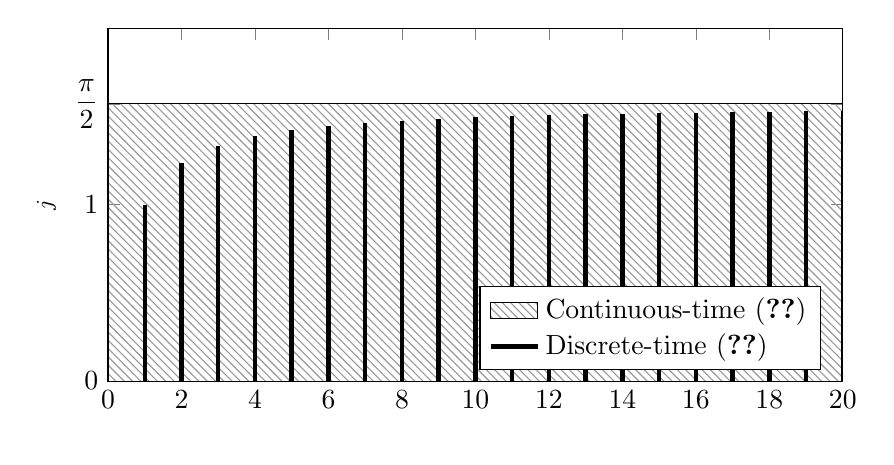
\begin{tikzpicture}[scale=1]
		\begin{axis}[xmin=0,xmax=20,ymin=0,ymax=2,
			ytick = {0,1,pi/2},yticklabels = {$ 0 $,$ 1 $,$ \dfrac{\pi}{2} $},
			tick label style={font=\normalsize},
			xlabel=$ \taun $,ylabel=$ \gpos_j\taun $,label style={font=\large},
			trig format plots=rad,
			legend pos=south east,legend style={font=\normalsize},legend cell align={left},
			width=.9\linewidth,height=.5\linewidth]
			\addplot[draw=black,pattern=north west lines,pattern color=black!40,area legend] (0,0) rectangle (20,pi/2);
			\addplot[domain=1:20,samples=20,mark=none,ycomb,ultra thick] {x*2*sin(pi/(2*(2*x+1)))};
			\addplot[draw=black,ultra thick] (20,0) -- (20,1);
			\legend{Continuous-time~\eqref{eq:cont-time-single-int-variance-condition},,Discrete-time~\eqref{eq:disc-time-single-int-stability-condition}};
		\end{axis}
	\end{tikzpicture}
	\caption{Stability regions of decoupled single integrators.}
	\label{fig:stability-region-single-int}
\end{figure}
					%!TEX ROOT = ../../centralized_vs_distributed.tex

\myParagraph{\titlecap{performance evaluation}}\label{sec:disc-time-single-int-moment-matching}
With fixed parameters,
the steady-state variance of each decoupled subsystem
can be computed numerically via the Wiener–Khintchine formula. % recalled in~\autoref{app:disc-time-single-int-variance-explicit}.
Also, for any given value of $ \taun $,
%gain-parametric 
a closed-form expression of the variance
%whose convexity can be easily assessed,
can be obtained via moment matching through a recursive formula, see~\cref{app:disc-time-single-int-variance-explicit}.
Such closed-form expressions have been used for our computational experiments illustrated in~\autoref{fig:opt-var}.
\textcolor{subsectioncolor}{Figure~\ref{fig:disc-time-var}} shows the typical profiles
of the variance function for decoupled subsystems with single- and double-integrator dynamics
(see~\eqref{eq:disc-time-single-int-decoupled} and~\eqref{eq:disc-time-double-int-decoupled} in~\cref{app:disc-time-single-int-variance-explicit},
respectively).
%For the one-dimensional case (single integrator),
%convexity of the variance function $ \var{\gpos_i} $ can be checked
%by studying the second derivative. % solving a system of inequalities.
%%over the decoupled subsystems.
%\autoref{fig:disc-time-var} shows the level curves of the variance,
%which looks convex also for the double integrator.

\begin{figure}
	\centering
	\begin{minipage}{.5\linewidth}
		\centering
		\includegraphics[width=\linewidth]{disc-time-single-int-var}
	\end{minipage}%
	\hfil
	\begin{minipage}{.5\linewidth}
		\centering
		\includegraphics[width=\linewidth]{disc-time-double-int-var-heatmap}
	\end{minipage}
	\caption{Typical profiles of the steady-state variance
		for decoupled discrete-time single integrators (left) and double integrators (right). %with $ \delayn \in \{5,7\} $.
%		The minima are highlighted by markers.
	}
	\label{fig:disc-time-var}
\end{figure}
	% \vspace{-0.5em}
\section{Conclusion}
% \vspace{-0.5em}
Recent advances in multimodal single-cell technology have enabled the simultaneous profiling of the transcriptome alongside other cellular modalities, leading to an increase in the availability of multimodal single-cell data. In this paper, we present \method{}, a multimodal transformer model for single-cell surface protein abundance from gene expression measurements. We combined the data with prior biological interaction knowledge from the STRING database into a richly connected heterogeneous graph and leveraged the transformer architectures to learn an accurate mapping between gene expression and surface protein abundance. Remarkably, \method{} achieves superior and more stable performance than other baselines on both 2021 and 2022 NeurIPS single-cell datasets.

\noindent\textbf{Future Work.}
% Our work is an extension of the model we implemented in the NeurIPS 2022 competition. 
Our framework of multimodal transformers with the cross-modality heterogeneous graph goes far beyond the specific downstream task of modality prediction, and there are lots of potentials to be further explored. Our graph contains three types of nodes. While the cell embeddings are used for predictions, the remaining protein embeddings and gene embeddings may be further interpreted for other tasks. The similarities between proteins may show data-specific protein-protein relationships, while the attention matrix of the gene transformer may help to identify marker genes of each cell type. Additionally, we may achieve gene interaction prediction using the attention mechanism.
% under adequate regulations. 
% We expect \method{} to be capable of much more than just modality prediction. Note that currently, we fuse information from different transformers with message-passing GNNs. 
To extend more on transformers, a potential next step is implementing cross-attention cross-modalities. Ideally, all three types of nodes, namely genes, proteins, and cells, would be jointly modeled using a large transformer that includes specific regulations for each modality. 

% insight of protein and gene embedding (diff task)

% all in one transformer

% \noindent\textbf{Limitations and future work}
% Despite the noticeable performance improvement by utilizing transformers with the cross-modality heterogeneous graph, there are still bottlenecks in the current settings. To begin with, we noticed that the performance variations of all methods are consistently higher in the ``CITE'' dataset compared to the ``GEX2ADT'' dataset. We hypothesized that the increased variability in ``CITE'' was due to both less number of training samples (43k vs. 66k cells) and a significantly more number of testing samples used (28k vs. 1k cells). One straightforward solution to alleviate the high variation issue is to include more training samples, which is not always possible given the training data availability. Nevertheless, publicly available single-cell datasets have been accumulated over the past decades and are still being collected on an ever-increasing scale. Taking advantage of these large-scale atlases is the key to a more stable and well-performing model, as some of the intra-cell variations could be common across different datasets. For example, reference-based methods are commonly used to identify the cell identity of a single cell, or cell-type compositions of a mixture of cells. (other examples for pretrained, e.g., scbert)


%\noindent\textbf{Future work.}
% Our work is an extension of the model we implemented in the NeurIPS 2022 competition. Now our framework of multimodal transformers with the cross-modality heterogeneous graph goes far beyond the specific downstream task of modality prediction, and there are lots of potentials to be further explored. Our graph contains three types of nodes. while the cell embeddings are used for predictions, the remaining protein embeddings and gene embeddings may be further interpreted for other tasks. The similarities between proteins may show data-specific protein-protein relationships, while the attention matrix of the gene transformer may help to identify marker genes of each cell type. Additionally, we may achieve gene interaction prediction using the attention mechanism under adequate regulations. We expect \method{} to be capable of much more than just modality prediction. Note that currently, we fuse information from different transformers with message-passing GNNs. To extend more on transformers, a potential next step is implementing cross-attention cross-modalities. Ideally, all three types of nodes, namely genes, proteins, and cells, would be jointly modeled using a large transformer that includes specific regulations for each modality. The self-attention within each modality would reconstruct the prior interaction network, while the cross-attention between modalities would be supervised by the data observations. Then, The attention matrix will provide insights into all the internal interactions and cross-relationships. With the linearized transformer, this idea would be both practical and versatile.

% \begin{acks}
% This research is supported by the National Science Foundation (NSF) and Johnson \& Johnson.
% \end{acks}
	
	\if0\mode
	\bibliographystyle{IEEEtran}
	\bibliography{bibfile}
	\else
	\input{centralized_vs_distributed_arxiv.bbl}
	\fi
	
	\appendix
	\numberwithin{equation}{subsection}
	%!TEX ROOT = ../centralized_vs_distributed.tex

\subsection{Proof of~\cref{prop:cont-time-double-int-stability}}\label{app:cont-time-double-int-stability}

%Let us consider the following generic scalar stochastic retarded linear system driven by a standard Brownian motion:
%\begin{equation}\label{eq:2nd-order-diff-eq}
%\dfrac{d^2\x{}{t}}{dt^2} + \gvel\dfrac{d\x{}{t}}{dt} + \gvel\gpos\x{}{t-1} = \dfrac{d\noise{}{t}}{dt}
%\end{equation}
The error dynamics equation with agent model~\eqref{eq:cont-time-double-int-model} reads
\begin{equation}\label{eq:multi-agent-state-space}
	\begin{array}{c}
		d\x{}{t} =
			\left(A_0\x{}{t} + A_1\x{}{t-1}\right)dt + Bd\noisebar{}{t}, \\[10pt]
		A_0 = \begin{bmatrix}
			0 & I\\
			0 & -\gvel I
		\end{bmatrix}, \
		A_1 = \begin{bmatrix}
			0 & 0\\
			-\gvel K & 0
		\end{bmatrix}, \
		B = \begin{bmatrix}
			0\\
			I
		\end{bmatrix},
	\end{array}
\end{equation}
with $ \noisebar{}{t} $ standard $ N $-dimensional Brownian motion.
The decoupling~\eqref{eq:agent-dynamics-1}
is obtained from~\eqref{eq:multi-agent-state-space} through
the change of basis $ \x{}{t} = (T\otimes I_2)\xtilde{}{t} $.
Rewriting~\eqref{eq:agent-dynamics-1} as a double integrator in state-space form 
with state $ \tilde{s}_j(\cdot) $ yields
\begin{equation}\label{eq:2n-order-system-state-space-1}
	\begin{array}{c}
		d\tilde{s}_j(t) = \left(F_0\tilde{s}_j(t)+F_{1j}\tilde{s}_j(t-1)\right)dt + Gd\noisebar{j}{t}, \\[5pt]
		 F_0 = \begin{bmatrix}
			0 & 1\\
			0 & -\gvel
		\end{bmatrix}, \ F_{1j} = \begin{bmatrix}
			0 & 0\\
			-\gvel\gpos_j & 0
		\end{bmatrix}, \ G = \begin{bmatrix}
			0\\
			1
		\end{bmatrix},
	\end{array}
\end{equation}
Stability of~\eqref{eq:multi-agent-state-space}
is equivalent to that of~\eqref{eq:2n-order-system-state-space-1} for all $ j $.
In the following, we drop the subscript $ j $ for the sake of readability.
%The first subsystem is stable for any $ \gvel > 0 $.
For positive eigenvalues $ \gpos $,~\eqref{eq:2n-order-system-state-space-1} is mean-square asymptotically stable
if $ \alpha_0 < 0 $ and unstable if $ \alpha_0 > 0 $~\cite{wangBoundedness}, where the \emph{spectral abscissa} is defined as
\begin{equation}\label{eq:2nd-order-system-stability-condition}
	\alpha_0 \doteq \sup\left\lbrace\Re(z) : z\in \mathbb{C}, \ h(z) = 0 \right\rbrace,
\end{equation}
and the \emph{characteristic polynomial} of~\eqref{eq:2n-order-system-state-space-1} is
\begin{equation}\label{eq:2n-order-system-chacteristic-polynomial}
	\begin{aligned}
		h(z) &\doteq \det\left(zI - F_0 - F_{1}\e^{-z}\right) = z^2 + \gvel z + \gvel\gpos\e^{-z}.  % = z^2 + \gvel z + \gvel\gpos\e^{-z}
%			 &= (z^2+\gvel z)\e^{z} + \gvel\gpos
	\end{aligned}
\end{equation}
A sufficient and necessary condition for all roots of $ h(z) $ to lie in the open left-hand half-plane is derived in~\cite{BAPTISTINI1997259}.
%and rewritten below for the sake of convenience.
\begin{thm}[\!\!\protect{\cite[Theorem 2.1]{BAPTISTINI1997259}}]\label{thm:stable-roots}
	Let the 2-vectors $v(b)=\left(p b, q-b^{2}\right), w(b)=$ $(\cos b, \sin b), b \geq 0,$ be given. If $r>0,$ a necessary and sufficient condition for all roots of the equation $h(z)=(z^2+pz+q)\e^{z} + r=0$ to have negative real part is that the orthogonality condition $v(b) \cdot w(b)=0,$ with $b \in \cup_{k=0}^{\infty}(2 k \pi,(2 k+1) \pi),$ implies $|v(b)|>r$.
\end{thm}
%In virtue of the above result, 
From~\cref{thm:stable-roots},~\eqref{eq:2n-order-system-state-space-1}
is asymptotically stable if the following implication holds for $b \in \cup_{k=0}^{\infty}(2 k \pi,(2 k+1) \pi)$,
\begin{equation}\label{eq:stability-condition-1}
	\gvel b\cos b - b^2\sin b = 0 \implies \gvel^2b^2+b^4>\gvel^2\gpos^2.
\end{equation}
In view of $ b \ge 0 $ and $ \sin b \ge 0 $,~\eqref{eq:stability-condition-1}
leads to~\eqref{eq:cont-time-double-int-stability-condition} after standard algebraic manipulations,
where we replace $ b $ with $ \beta = \min b \in (0,\nicefrac{\pi}{2}) $.
The inequality can be rewritten as
\begin{equation}\label{eq:stability-condition-lambda}
	\gpos < \dfrac{\beta}{\sin\beta} \doteq \phi(\gvel),
\end{equation}
where the definition of $ \phi(\cdot) $ follows from the implicit function theorem
applied to $ F(\gvel,\beta) \doteq \beta\tan\beta - \gvel $,
which states that $ F(\gvel,\beta) = 0 $ if and only if $ \beta = \varphi(\gvel) $ and
%$ \varphi'(\cdot), \varphi''(\cdot) $ can be explicitly computed, with
\begin{equation}\label{eq:varphi-of-eta-derivative}
	\varphi'(\gvel) = \dfrac{\cos^2\left(\varphi(\gvel)\right)}{\varphi(\gvel) + \sin\left(\varphi(\gvel)\right)\cos\left(\varphi(\gvel)\right)}
\end{equation}
Tedious but straightforward calculations on the first and second derivatives %$ \phi'(\gvel) $ and $ \phi''(\gvel) $
show that $ \phi(\gvel) $ is concave increasing for any $ \gvel > 0 $.
The limits at $ 0 $ and $ +\infty $ can be easily computed
by noting that
\begin{equation}\label{eq:stability-condition-limits}
	\beta_0\doteq\varphi(0) = 0, \quad \beta_\infty\doteq\lim_{\gvel\rightarrow+\infty}\varphi(\gvel) = \dfrac{\pi}{2}.
\end{equation}





	%!TEX ROOT = ../centralized_vs_distributed.tex

\subsection{\titlecap{derivation of first-order reduced model for continuous-time double integrators}}\label{app:time-scale-separation}

We now show that subsystem~\eqref{eq:agent-dynamics-1}
can be approximated to first-order dynamics
%when the control input is sufficiently powerful.
when the gain $ \gvel $ is sufficiently high.
%We first rewrite~\eqref{eq:agent-dynamics-1} in state-space form:
%\begin{equation}\label{eq:2n-order-system-state-space}
%\begin{aligned}
%d\x{}{t} &= \z{}{t}dt\\
%d\z{}{t} &= \left(-\gvel \z{}{t} - \gvel\gpos \x{}{t-1}\right)dt + d\noise{}{t}
%\end{aligned}
%\end{equation}
Let us consider~\eqref{eq:2n-order-system-state-space-1} with state $ \tilde{s}(t) = [\xtilde{}{t},\ztilde{}{t}]^\top $.
Assume that the feedback gain $ \gvel $ is large,
so that the variable $ \ztilde{}{t} $ evolves faster than $ \xtilde{}{t} $.
We can then approximate the dynamics of $ \ztilde{}{t} $ 
by letting $ \xtilde{}{t-1} \equiv x_0 $ be constant overtime,
\begin{equation}\label{eq:z-dynamics-with-constant-x}
d\ztilde{}{t} = \left(-\gvel \ztilde{}{t} - \gvel\gpos x_0\right)dt + d\noise{}{t}.
\end{equation}
\cref{eq:z-dynamics-with-constant-x} defines a standard Ornstein–Uhlenbeck process,
\begin{equation}\label{eq:z-solution-constant-x}
\ztilde{}{t} \sim \gauss\left( \e^{-\gvel t}(\ztilde{}{0} + \gpos x_0) - \gpos x_0, \dfrac{1}{2\gvel}\left(1-\e^{-2\gvel t}\right) \right).
\end{equation}
In view of the time-scale separation,
we assume that~\eqref{eq:z-solution-constant-x} holds (with $ \xtilde{}{t-1} $ constant) till $ \ztilde{}{t} $ settles at steady state, %the limit, tends to
\begin{equation}\label{eq:z-solution-constant-x-limit-gvel}
\lim_{t \rightarrow +\infty}\ztilde{}{t} = \tilde{z}_{\infty} \sim \gauss\left( - \gpos x_0, \dfrac{1}{2\gvel} \right).
\end{equation}
Using~\eqref{eq:z-solution-constant-x-limit-gvel},
we now approximate the dynamics of $ \xtilde{}{t} $ %in~\eqref{eq:agent-dynamics-1}
as if $ \ztilde{}{t} $ reached the steady state instantaneously,
\begin{equation}\label{eq:x-dynamics-1st-order}
d\xtilde{}{t} \approx \tilde{z}_{\infty}dt = -\gpos\xtilde{}{t-1}dt + dn(t),
\end{equation}
where 
%the drift only contains the dominant term $ -\gpos\x{}{t-1} $ and
the diffusion is embedded into the Brownian noise $ n(t) $ with variance proportional to $ \nicefrac{1}{\gvel} $.
In particular, as $ \gvel \rightarrow +\infty $,
$ \tilde{z}_{\infty} \xrightarrow{a.s.} - \gpos x_0 $
and~\eqref{eq:x-dynamics-1st-order} tends to deterministic dynamics.
	%!TEX ROOT = ../centralized_vs_distributed.tex

\newpage
\subsection{\titlecap{Computation of suboptimal variance for continuous-time single integrators}}\label{app:cont-time-single-int-suboptimal-variance-computation}

%Consider the suboptimal gain $ \tilde{k}^* $ as per~\cref{prop:subopt-gain}.
The $ N $ suboptimal eigenvalues have expression (cf.~\cite{circulant})
\begin{equation}\label{eq:eigenvaluesCirculant}
	\tilde{\gpos}_j^* = 2\tilde{k}^* \left(n - \sum_{\ell=1}^n\cos\left(\dfrac{2\pi (j-1) \ell}{N}\right)\right), %, \ j=1,\dots,N
\end{equation}
which we write as $ \tilde{\gpos}_j^* = g_j(n)\tilde{k}^* $.
Being $ \tilde{k}^* = \tilde{\alpha}^*(n) \opteig $
according to~\cref{prop:subopt-gain},
we write $ \tilde{\gpos}_j^* = \tilde{c}_j^*(n)\opteig $ with $  \tilde{c}_j^*(n) \doteq g_j(n)\tilde{\alpha}^*(n) $.
Then, each subsystem~\eqref{eq:cont-time-single-int-subsystem} has variance %$ \sigma_{\textit{ss}}^{2,I}(\tilde{\gpos}_j^*) $ is
\begin{align}\label{eq:optimalVarianceLambda_i}
	\varx{\tilde{\lambda}_j^*}{I} = \dfrac{1+\sin(\tilde{\lambda}_j^* \taun)}{2\tilde{\lambda}_j^*\cos(\tilde{\lambda}_j^* \taun)}
	\overset{(i)}{=} \underbrace{\dfrac{1+\sin(\tilde{c}_j^*(n)\beta^*)}{2\tilde{c}_j^*(n)\beta^*\cos(\tilde{c}_j^*(n)\beta^*)}}_{\doteq\tilde{C}_{j}^*(n)}\taun 
%	= \tilde{C}_{j}^*(n)\taun,
%	\begin{split}
%		\varx{\tilde{\lambda}_j^*}{I} &= \dfrac{1+\sin(\tilde{\lambda}_j^* \taun)}{2\tilde{\lambda}_j^*\cos(\tilde{\lambda}_j^* \taun)} \\
%		%&= \dfrac{1+\sin(g(n)\tilde{c}^*(n)\opteig \taun)}{2g(n)\tilde{c}^*(n)\opteig\cos(g_n)\tilde{c}^*(n)\opteig \taun)} \\
%		&\overset{(i)}{=} \dfrac{1+\sin(\tilde{c}_j^*(n)\beta^*)}{2\tilde{c}_j^*(n)\beta^*\cos(\tilde{c}_j^*(n)\beta^*)}\taun = \tilde{C}_{j}^*(n)\taun,
%	\end{split}
\end{align}
where~\eqref{eq:optimal-variance-closed-form} is used in \textit{(i)}.
%$ a_i^*(n) \doteq g_i(n)\tilde{c}^*(n) $ and
%$ \tilde{C}_i^*(n) $ multiplies $ \taun $ in the third line of~\eqref{eq:optimalVarianceLambda_i}.
%The scalar variance can then be written as
%\begin{equation}\label{eq:scalarVarianceSumExplicit}
%\optvarx = \sum_{i=2}^N \tilde{C}_i^*(n)\taun = \tilde{C}^*(n)f(n)\tau_{\textit{min}}
%\end{equation}
%where $ \displaystyle \tilde{C}^*(n) \doteq \sum_{i=2}^N \tilde{C}_i^*(n) $.
	%!TEX ROOT = ../centralized_vs_distributed.tex

\subsection{\titlecap{stability conditions for discrete-time systems}}\label{app:disc-time-single-int-stability}

\begin{figure}
	\centering
	%!TEX ROOT = ../centralized_vs_distributed.tex

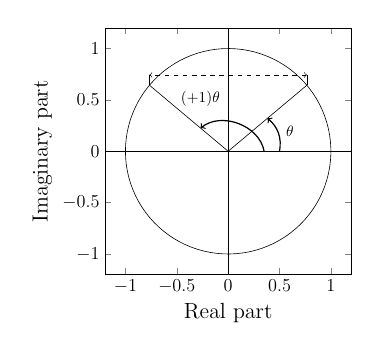
\begin{tikzpicture}[scale=.55]
	\begin{axis}[
		xlabel = Real part,
		ylabel = Imaginary part,
		axis equal image,
		ymin = -1.2,
		ymax = 1.2,
		xmin = -1.2,
		xmax = 1.2]
		\addplot [domain=-180:180, samples=100] ({cos(x)},{sin(x)});
		\draw (-1.2,0) -- (1.2,0);
		\draw (0,-1.2) -- (0,1.2);
		\draw (0,0) -- ({cos(40)},{sin(40)});
		\draw (0,0) -- ({-cos(40)},{sin(40)});
		\path[->,thick] (.5,0) edge[bend right] node [left] {}  ({.5*cos(40)},{.5*sin(40)});
		\path[->,thick] (.35,0) edge[bend right=60] node [left] {}  ({-.35*cos(40)},{.35*sin(40)}) ;
		\node at (.6,.2) {$ \delayn \theta $};
		\node at (-.27,.51) {$ (\delayn+1) \theta $};	
		\draw[<->,dashed] ({cos(40)},{sin(40)+.1}) -- ({-cos(40)},{sin(40)+.1});
		\draw ({cos(40)},{sin(40)+.1}) -- ({cos(40)},{sin(40)});
		\draw (-{cos(40)},{sin(40)+.1}) -- (-{cos(40)},{sin(40)});
		\node at (0.05,{sin(40)+.2}) {$ \gpos $};
	\end{axis}
\end{tikzpicture}
	\caption{A solution of~\eqref{eq:disc-time-single-int-uint-poles-system} in the complex plane.}
	\label{fig:disc-time-single-int-unit-poles}
\end{figure}

\myParagraph{\titlecap{General case}}
In the following, we replace $ \taun $ with $ \delayn $ % drop the subscript from $ \taun $
for the sake of readability.
For the single-integrator case, decoupling the error dynamics yields scalar subsystems of the form
\begin{equation}\label{eq:disc-time-single-int-decoupled}
	\xtilde{}{k+1} = \xtilde{}{k} - \gpos\xtilde{}{k-\tau} + \noisetilde{}{k}.
\end{equation}
The characteristic polynomial $ h(z) $ of~\eqref{eq:disc-time-single-int-decoupled} is obtained by
applying the lag operator $ z $
such that $ \xtilde{}{k}h(z) = \noisetilde{}{k} $,
\begin{equation}\label{eq:disc-time-single-int-characteristic-polinomial}
	h(z) = z - 1 + \gpos z^{-\tau}.
\end{equation}
Similarly, the double-integrator decoupled subsystems are
\begin{equation}\label{eq:disc-time-double-int-decoupled}
%	\xtilde{i}{k+1} = (2-\gvel)\xtilde{i}{k} - (1-\gvel)\xtilde{i}{k-1} - \gvel\gpos\xtilde{i}{k-\taun-1} + \noisetilde{i}{k}
	\begin{aligned}
		\xtilde{}{k+1} &= \xtilde{}{k} + \ztilde{}{k}\\
		\ztilde{}{k+1} &= (1-\gvel)\ztilde{}{k} - \gvel\gpos\xtilde{}{k-\tau} + \noisetilde{}{k},
	\end{aligned}
\end{equation}
with characteristic polynomial
\begin{equation}\label{eq:disc-time-double-int-characteristic-polinomial}
	h(z) = z-2+\gvel+(1-\gvel)z^{-1}+\gvel\gpos z^{-\tau-1}.
\end{equation}
For positive $ \gpos $, stability of~\eqref{eq:disc-time-single-int-decoupled}--\eqref{eq:disc-time-double-int-decoupled}
can be assessed via the Jury stability criterion,
which provides necessary and sufficient conditions for
the roots of~\eqref{eq:disc-time-single-int-characteristic-polinomial} and~\eqref{eq:disc-time-double-int-characteristic-polinomial}
to lie inside the unit circle %in the complex plane
in the form of inequalities involving the coefficients of $ h(z) $.
Being the latter polynomial in $ \gvel $ and $ \gpos $,
the Jury criterion %applied to~\eqref{eq:disc-time-single-int-model}--\eqref{eq:disc-time-double-int-model}
yields $ \Theta(N\tau) $ polynomial inequalities in the feedback gains,
which can be computed through standard software tools.

\myParagraph{Proof of~\cref{prop:disc-time-single-int-stability}}
\cref{eq:disc-time-single-int-characteristic-polinomial} can be studied as a root locus
by varying the gain $ \gpos $.
In particular, $ \gpos = 0 $ yields
a multiple root at $ z_1^* = 0 $ and a simple root at $ z_2^* = 1 $.
Negative values of $ \gpos $ are discarded as they push the latter outside the unit circle.
As $ \gpos $ increases,
the branches leave the unit ball along their asymptotes.
%Notice that, in view of the structure of the root locus,
The admissible values for $ \gpos $ are upper bounded by a threshold gain $ \gpos_{\textit{th}} $
beyond which some roots leave the unit ball.
In particular, we are interested in the minimum gain for which at least one root lies exactly on the unit circle.
Thus, we are looking for roots of~\eqref{eq:disc-time-single-int-characteristic-polinomial}
of the form $ z = \e^{j\theta} $,
\begin{equation}\label{eq:disc-time-single-int-unit-poles-eq}
	\e^{j(\delayn+1)\theta} - \e^{j\delayn\theta} + \gpos = 0.
\end{equation}
\cref{eq:disc-time-single-int-unit-poles-eq} can be equivalently written as the system
\begin{equation}\label{eq:disc-time-single-int-uint-poles-system}
	\begin{cases}
		\cos((\delayn+1)\theta) - \cos(\delayn\theta) + \gpos = 0\\
		\sin((\delayn+1)\theta) = \sin(\delayn\theta).
	\end{cases}
\end{equation}
\autoref{fig:disc-time-single-int-unit-poles} depicts a solution of~\eqref{eq:disc-time-single-int-uint-poles-system} for $ \sin(\delayn\theta) > 0 $.
The case $ \sin(\delayn\theta)<0 $ is analogous
and is omitted.
Further, the solution $ (\delayn+1)\theta = \delayn\theta $
can be discarded because it implies $ \gpos = 0 $ and thus prevents asymptotic stability.
%On the other hand, 
%Therefore, we only focus on the case $ \sin(\delayn\theta)>0 $. % depicted in the left box in~\autoref{fig:disc-time-single-int-unit-poles}.
From basic trigonometric arguments (c.f.~\autoref{fig:disc-time-single-int-unit-poles}),
the second equation in~\eqref{eq:disc-time-single-int-uint-poles-system} implies
\begin{equation}\label{eq:disc-time-single-int-theta}
	\delayn\theta + \dfrac{\theta}{2} = \dfrac{\pi}{2} + 2k\pi \ \longrightarrow \ \theta = \dfrac{\pi+4k\pi}{2\delayn+1}, \quad 
\end{equation}
where we impose $ \theta \in [0,\pi] $
and thus $ k\in\{0,\dots,\floor{\nicefrac{\delayn}{2}}\} $.
This includes all possible cases,
because the roots of~\eqref{eq:disc-time-single-int-characteristic-polinomial} come in complex conjugates pairs.
From~\eqref{eq:disc-time-single-int-theta},
the first equation in~\eqref{eq:disc-time-single-int-uint-poles-system},
and the fact $ \cos((\delayn+1)\theta) = - \cos(\delayn\theta) $,
we retrieve
\begin{equation}\label{eq:disc-time-single-int-unit-roots-gain}
	\gpos = 2\cos\left(\dfrac{\pi\delayn+4k\pi\delayn}{2\delayn+1}\right).
\end{equation}
The right-hand term in~\eqref{eq:disc-time-single-int-unit-roots-gain} is monotone increasing in $ k $.
Indeed, taking the argument of the cosine modulus $ 2\pi $ yields
\begin{equation}\label{eq:disc-time-single-int-angle-modulus}
	\dfrac{\pi\delayn+4k\pi\delayn}{2\delayn+1} \ \mod \ 2\pi = \dfrac{\pi\delayn-2k\pi}{2\delayn+1} \in \left[0,\dfrac{\pi}{2}\right),
\end{equation}
which is nonnegative and monotone decreasing in $ k $ for any $ \tau $.
Finally, the upper bound for the gain $ \gpos $ is given by
\begin{equation}\label{eq:disc-time-single-int-threshold-gain}
	\gpos_{\textit{th}} = \min_k2\cos\left(\dfrac{\pi\delayn+4k\pi\delayn}{2\delayn+1}\right) = 2\cos\left(\dfrac{\pi\delayn}{2\delayn+1}\right).
% 2\sin\left(\dfrac{\pi}{2}\dfrac{1}{2\delayn+1}\right)
\end{equation}



	\if0\mode
	%!TEX ROOT = ../centralized_vs_distributed.tex

\subsection{\titlecap{variance computation for discrete-time systems}}\label{app:disc-time-single-int-variance-explicit}

\myParagraph{Wiener--Kintchine Formula}
Given any fixed values of delay and feedback gains,
the steady-state variance $ \varx{\gpos}{I} $ or $ \varx{\gvel,\gpos}{II} $ of the decoupled subsystems can be computed numerically by
\begin{equation}\label{eq:disc-time-variance-integral}
	\dfrac{1}{2\pi}\int_{-\pi}^{+\pi}\dfrac{d\theta}{|h(\e^{j\theta})|^2},
\end{equation}
where the characteristic polynomial $ h(z) $
is~\eqref{eq:disc-time-single-int-characteristic-polinomial} or~\eqref{eq:disc-time-double-int-characteristic-polinomial}.

\myParagraph{Single Integrator Model}
The moment-matching method applied to subsystem~\eqref{eq:disc-time-single-int-decoupled} yields 
a linear system of equations in the variables $ (\rho_0,...,\rho_\delayn) $,
where $ \rho_t \doteq \mathbb{E}[\xtilde{}{k}\xtilde{}{k\pm t}] $:
\begin{subequations}\label{eq:disc-time-single-int-moment-matching-eqs}
	\begin{align}
		\rho_0 &= \mathbb{E}[\xtilde{}{k+1}^2] = \rho_0 + \gpos^2\rho_0 + 1 - 2\gpos\rho_\delayn \label{eq:disc-time-single-int-first-moment-eq}\\
		\rho_1 &= \mathbb{E}[\xtilde{}{k+1}\xtilde{}{k}] = \rho_0 - \gpos\rho_\delayn \label{eq:disc-time-single-int-yule-walker-eqs-1}\\
		&\hspace{2mm}\vdots \nonumber \\
		\rho_\delayn &= \rho_{\delayn-1} - \gpos\rho_1, \label{eq:disc-time-single-int-yule-walker-eqs-2}
	\end{align}
\end{subequations}
where~\eqref{eq:disc-time-single-int-yule-walker-eqs-1}--\eqref{eq:disc-time-single-int-yule-walker-eqs-2} are the Yule-Walker equations.
%associated to the decoupled subsystem~\eqref{eq:disc-time-single-int-decoupled}.
System~\eqref{eq:disc-time-single-int-moment-matching-eqs}
can be written compactly as $ A^{(\tau)}\rho = e_1 $, 
where $ \rho^\top = [\rho_0,\dots,\rho_{\delayn}]$,
$ e_1 $ is the canonical vector in $ \Real{\delayn+1} $ with nonzero first coordinate,
and $ A^{(\tau)}\in\Real{(\delayn+1)\times(\delayn+1)} $ gathers all coefficients of equations in~\eqref{eq:disc-time-single-int-moment-matching-eqs}.
%with
%\begin{equation}\label{eq:explicit-variance-matrix-A}
%A^{(\tau)} = \begin{bmatrix}
%-\gpos^2 &   		&     		& 		 &   	  & 2\gpos\\
%1 		 & -1 		&     		& 		 &    	  & -\gpos\\
%& 	\ddots	& \ddots	&  		 & \iddots&  \\
%& 			& 			&		 & 		  &  \\
%& 			& 			&		 & 		  &  \\
%& -\gpos	& 			& 		 & 1 	  & -1
%\end{bmatrix}.
%\end{equation}
%In particular, when $ \delayn $ is odd, the $ (\ceil{\nicefrac{\delayn}{2}} + 1) $-th row is
%\begin{equation}\label{eq:app-explicit-variance-matrix-A-mid-row-odd}
%	\left[\!\begin{array}{cccccccc}
%	0 & \dots & 0 & 1 & -1-\gpos & 0 & \dots & 0
%	\end{array}\!\right],
%\end{equation}
%while, when $ \delayn $ is even, the $ (\nicefrac{\delayn}{2} + 2) $-th row is
%\begin{equation}\label{eq:app-explicit-variance-matrix-A-mid-row-even}
%	\left[\!\begin{array}{cccccccc}
%		0 & \dots & 0 & 1-\gpos & -1 & 0 & \dots & 0
%	\end{array}\!\right].
%\end{equation}
%where we highlight the dependence on the delay in view of the recursive characterization of $ \rho_0 $.
It can be seen that $ A^{(\tau)} $ is full rank for all $ \delayn \ge 1 $ and thus~\eqref{eq:disc-time-single-int-moment-matching-eqs} has a unique solution.
In particular, we are interested in the autocorrelation $ \rho_0 = \varx{\gpos}{I} $,
which is given by
the ratio between the minor associated with the top-left element of $ A^{(\tau)} $,
named $ n_\delayn \doteq M^{(\tau)}_{1,1} $, and the determinant $ d_\delayn \doteq \det(A^{(\tau)}) $.
Specifically, $ \rho_0 $ is a rational function in $ \gpos $
and can be computed in closed form by a symbolic solver
given any value of $ \delayn $.

Further, $ n_{\delayn} $ and $ d_{\delayn} $ can be explicitly computed %recursively via an inductive argument on the delay $ \delayn $, 
by leveraging a recursive nested structure of the matrix $ A $.
%\begin{equation}\label{eq:recursive-matrix}
%	A^{(\delayn)} = \tikz[baseline=(M.west)]{%
%		\node[matrix of math nodes,matrix anchor=west,left delimiter={[},right delimiter={]},ampersand replacement=\&] (M) {%
%		-\gpos^2\&			\&			\&							\& 							\&						 \&	-2\gpos		\\
%			1 	\& -1  		\&    		\&							\& 							\& 						 \&	  			\\
%				\&  1  		\&  -1		\&	  						\&      					\& 						 \& -\gpos   	\\
%				\&    		\&   1 		\& \textcolor{white}{t1}	\& 							\& 						 \&				\\
%				\&			\&			\&							\& \tilde{A}^{(\delayn-4)}	\&						 \&				\\
%				\& 			\&	  		\& 							\&	 						\& \textcolor{white}{t1} \&				\\
%				\& 		    \&   -\gpos	\&							\&							\& 1					 \&	-1			\\
%				\& 	-\gpos	\&	  		\&							\&							\&						 \&	1			\\			
%		};
%		\node[draw,fit=(M-3-3)(M-7-7),inner sep=-1pt] {};
%		\node[draw,fit=(M-4-4)(M-6-6),inner sep=-1pt] {};
%	}.
%\end{equation}
%where $ \tilde{A}^{(\delayn)} $ is the submatrix of $ A^{(\delayn)} $ obtained by removing its first row and column
%such that $ M^{(\delayn)}_{1,1} = \det(\tilde{A}^{(\delayn)}) $,
%and the matrices $ \tilde{A}^{(\delayn-2)} $ and $ \tilde{A}^{(\delayn-4)} $ are framed in~\eqref{eq:recursive-matrix}.
The solution obeys the following recursive expression in $ \delayn $:
%\begin{prop}\label{prop:disc-time-single-int-variance-explicit}
\begin{subequations}\label{eq:disc-time-single-int-variance-explicit}
	\begin{gather}
		n_\delayn = \begin{dcases}
			(-1-\gpos)n_{\delayn-1} + \tilde{n}_{\delayn-1} & \mbox{if } \delayn \mbox{ odd}\\
			-(1-\gpos)n_{\delayn-1} - \gpos\tilde{n}_{\delayn-1} & \mbox{if }\delayn \mbox{ even},\\
		\end{dcases} \label{eq:disc-time-single-int-variance-explicit-numerator}\\
		\tilde{n}_{\delayn} = (2-\gpos^2)\tilde{n}_{\delayn-2} - \tilde{n}_{\delayn-4}, \label{eq:disc-time-single-int-variance-explicit-numerator-rem}\\
		d_\delayn = d_{\delayn-2} - \gpos^2\left(n_\delayn+n_{\delayn-2}\right), \label{eq:disc-time-single-int-variance-explicit-denominator}\\
		\tilde{n}_{-3} = -1+\gpos^2, \ \tilde{n}_{-2} = \gpos^2, \ \tilde{n}_{-1} = -1, \ \tilde{n}_0 = 0, \\
		n_{-1} = 0, \ n_0 = 1, \ d_{-1} = -2\gpos, \ d_0 = 2\gpos-\gpos^2.
	\end{gather}
\end{subequations}
Detailed derivation of~\eqref{eq:disc-time-single-int-variance-explicit}
is given in the technical report~\cite{2021arXiv210900359B}.
Given $ \delayn $,
convexity of $ \rho_0 $ in $ \gpos $ can be assessed by checking the sign
of the second derivative in the stability region.
This reduces to a system of inequalities
which can be solved, \eg by \texttt{solve\_rational\_inequalities} in Python.
The variance was proved strictly convex for all tried delays.

\myParagraph{\titlecap{double integrator model}}
System~\eqref{eq:disc-time-double-int-decoupled} yields the following
$ \delayn+2 $ coupled moment-matching equations,
%The moment-matching system associated with~\eqref{eq:disc-time-double-int-decoupled}
%has $ \delayn+2 $ variables $ (\rho_0,\dots,\rho_{\delayn+1}) $ and is composed of the following equations:
\begin{subequations}\label{eq:disc-time-double-int-moment-matching-eqs}
	\begin{align}
		\begin{split}
			\rho_0 &= [(2-\gvel)^2 + (1-\gvel)^2 + \gvel^2\gpos^2]\rho_0 - 2(2-\gvel)(1-\gvel)\rho_1 \\
			& + 2(1-\gvel)\gvel\gpos\rho_\delayn - 2(2-\gvel)\gvel\gpos\rho_{\delayn+1} + 1 \label{eq:disc-time-double-int-first-moment-eq}
		\end{split}\\
		\rho_1 &= (2-\gvel)\rho_0 - (1-\gvel)\rho_1 - \gvel\gpos\rho_{\delayn+1} \label{eq:disc-time-double-int-yule-walker-eqs-1}\\
		&\hspace{2mm}\vdots \nonumber \\
		\rho_{\delayn+1} &= (2-\gvel)\rho_\delayn - (1-\gvel)\rho_{\delayn-1} - \gvel\gpos\rho_1, \label{eq:disc-time-double-int-yule-walker-eqs-2}
	\end{align}
\end{subequations}
with~\eqref{eq:disc-time-double-int-yule-walker-eqs-1}--\eqref{eq:disc-time-double-int-yule-walker-eqs-2} the associated Yule-Walker equations.
%associated with~\eqref{eq:disc-time-double-int-decoupled}.
Analogous analysis to single-integrator model can be performed.
	\else
	%!TEX ROOT = ../centralized_vs_distributed.tex

\subsection{\titlecap{variance computation for discrete-time systems}}\label{app:disc-time-single-int-variance-explicit}

\myParagraph{Wiener--Kintchine Formula}
Given any fixed values of delay and feedback gains,
the steady-state variance $ \varx{\gpos}{I} $ or $ \varx{\gvel,\gpos}{II} $ of the decoupled subsystems can be computed numerically by
\begin{equation}\label{eq:disc-time-variance-integral}
	\dfrac{1}{2\pi}\int_{-\pi}^{+\pi}\dfrac{d\theta}{|h(\e^{j\theta})|^2},
\end{equation}
where the characteristic polynomial $ h(z) $
is~\eqref{eq:disc-time-single-int-characteristic-polinomial} or~\eqref{eq:disc-time-double-int-characteristic-polinomial}.

\myParagraph{\titlecap{single integrator model}}
The moment-matching method applied to the subsystem~\eqref{eq:disc-time-single-int-decoupled} yields 
a linear system of equations in the variables $ (\rho_0,...,\rho_\delayn) $,
where $ \rho_t \doteq \mathbb{E}[\xtilde{}{k}\xtilde{}{k\pm t}] $:
\begin{subequations}\label{eq:disc-time-single-int-moment-matching-eqs}
	\begin{align}
		\rho_0 &= \mathbb{E}[\xtilde{}{k+1}^2] = \rho_0 + \gpos^2\rho_0 + 1 - 2\gpos\rho_\delayn \label{eq:disc-time-single-int-first-moment-eq}\\
		\rho_1 &= \mathbb{E}[\xtilde{}{k+1}\xtilde{}{k}] = \rho_0 - \gpos\rho_\delayn \label{eq:disc-time-single-int-yule-walker-eqs-1}\\
		&\hspace{2mm}\vdots \nonumber \\
		\rho_\delayn &= \rho_{\delayn-1} - \gpos\rho_1, \label{eq:disc-time-single-int-yule-walker-eqs-2}
	\end{align}
\end{subequations}
where~\eqref{eq:disc-time-single-int-yule-walker-eqs-1}--\eqref{eq:disc-time-single-int-yule-walker-eqs-2} are the Yule-Walker equations.
%associated to the decoupled subsystem~\eqref{eq:disc-time-single-int-decoupled}.
System~\eqref{eq:disc-time-single-int-moment-matching-eqs}
can be written compactly as $ A^{(\tau)}\rho = e_1 $, where
$ \rho^\top = [\rho_0,\dots,\rho_{\delayn}]$,
$ e_1 $ is the canonical vector in $ \Real{\delayn+1} $ with nonzero first coordinate and $ A^{(\tau)}\in\Real{(\delayn+1)\times(\delayn+1)} $ with
\begin{equation}\label{eq:explicit-variance-matrix-A}
	A^{(\tau)} = \begin{bmatrix}
		-\gpos^2 &   		&     		& 		 &   	  & 2\gpos\\
		1 		 & -1 		&     		& 		 &    	  & -\gpos\\
		& 	\ddots	& \ddots	&  		 & \iddots&  \\
		& 			& 			&		 & 		  &  \\
		& 			& 			&		 & 		  &  \\
		& -\gpos	& 			& 		 & 1 	  & -1
	\end{bmatrix}.
\end{equation}
In particular, when $ \delayn $ is odd, the $ (\ceil{\nicefrac{\delayn}{2}} + 1) $-th row is
\begin{equation}\label{eq:app-explicit-variance-matrix-A-mid-row-odd}
	\left[\!\begin{array}{cccccccc}
		0 & \dots & 0 & 1 & -1-\gpos & 0 & \dots & 0
	\end{array}\!\right],
\end{equation}
while, when $ \delayn $ is even, the $ (\nicefrac{\delayn}{2} + 2) $-th row is
\begin{equation}\label{eq:app-explicit-variance-matrix-A-mid-row-even}
	\left[\!\begin{array}{cccccccc}
		0 & \dots & 0 & 1-\gpos & -1 & 0 & \dots & 0
	\end{array}\!\right].
\end{equation}
%where we highlight the dependence on the delay in view of the recursive characterization of $ \rho_0 $.
Notice that $ A^{(\tau)} $ is full rank for all $ \delayn \ge 1 $ and thus~\eqref{eq:disc-time-single-int-moment-matching-eqs} can be solved uniquely.
In particular, we are interested in the autocorrelation $ \rho_0 = \varx{\gpos}{I} $,
which is given by
the ratio between the minor associated with the top-left element of $ A^{(\tau)} $,
named $ n_\delayn \doteq M^{(\tau)}_{1,1} $, and the determinant $ d_\delayn \doteq \det(A^{(\tau)}) $.
Specifically, $ \rho_0 $ is a rational function in $ \gpos $
and can be computed in closed form by a symbolic solver
given any value of $ \delayn $.

Further, $ n_{\delayn} $ and $ d_{\delayn} $ can be computed %recursively via an inductive argument on the delay $ \delayn $, 
by leveraging the following nested structure of the matrix $ A^{(\delayn)} $:
\begin{equation}\label{eq:recursive-matrix}
	A^{(\delayn)} = \tikz[baseline=(M.west)]{%
		\node[matrix of math nodes,matrix anchor=west,left delimiter={[},right delimiter={]},ampersand replacement=\&] (M) {%
			-\gpos^2\&			\&			\&							\& 							\&						 \&	-2\gpos		\\
			1 	\& -1  		\&    		\&							\& 							\& 						 \&	  			\\
			\&  1  		\&  -1		\&	  						\&      					\& 						 \& -\gpos   	\\
			\&    		\&   1 		\& \textcolor{white}{t1}	\& 							\& 						 \&				\\
			\&			\&			\&							\& \tilde{A}^{(\delayn-4)}	\&						 \&				\\
			\& 			\&	  		\& 							\&	 						\& \textcolor{white}{t1} \&				\\
			\& 		    \&   -\gpos	\&							\&							\& 1					 \&	-1			\\
			\& 	-\gpos	\&	  		\&							\&							\&						 \&	1			\\			
		};
		\node[draw,fit=(M-3-3)(M-7-7),inner sep=-1pt] {};
		\node[draw,fit=(M-4-4)(M-6-6),inner sep=-1pt] {};
	},
\end{equation}
where $ \tilde{A}^{(\delayn)} $ is the submatrix of $ A^{(\delayn)} $ obtained by removing its first row and column
such that $ M^{(\delayn)}_{1,1} = \det(\tilde{A}^{(\delayn)}) $,
and the matrices $ \tilde{A}^{(\delayn-2)} $ and $ \tilde{A}^{(\delayn-4)} $ are framed in~\eqref{eq:recursive-matrix}.

The solution obeys the following recursive expression in $ \delayn $:
%\begin{prop}\label{prop:disc-time-single-int-variance-explicit}
\begin{subequations}\label{eq:disc-time-single-int-variance-explicit}
	\begin{gather}
		n_\delayn = \begin{dcases}
			(-1-\gpos)n_{\delayn-1} + \tilde{n}_{\delayn-1} & \mbox{if } \delayn \mbox{ odd}\\
			-(1-\gpos)n_{\delayn-1} - \gpos\tilde{n}_{\delayn-1} & \mbox{if }\delayn \mbox{ even},\\
		\end{dcases} \label{eq:disc-time-single-int-variance-explicit-numerator}\\
		\tilde{n}_{\delayn} = (2-\gpos^2)\tilde{n}_{\delayn-2} - \tilde{n}_{\delayn-4}, \label{eq:disc-time-single-int-variance-explicit-numerator-rem}\\
		d_\delayn = d_{\delayn-2} - \gpos^2\left(n_\delayn+n_{\delayn-2}\right), \label{eq:disc-time-single-int-variance-explicit-denominator}\\
		\tilde{n}_{-3} = -1+\gpos^2, \ \tilde{n}_{-2} = \gpos^2, \ \tilde{n}_{-1} = -1, \ \tilde{n}_0 = 0, \\
		n_{-1} = 0, \ n_0 = 1, \ d_{-1} = -2\gpos, \ d_0 = 2\gpos-\gpos^2.
	\end{gather}
\end{subequations}

\cref{eq:disc-time-single-int-variance-explicit} can be proved by an inductive argument
on the delay $ \delayn $.

\myParagraph{Numerator}
We demonstrate the formula for odd delays $ \delayn = 2k+1, k\in\mathbb{N} $.
The other case can be obtained similarly and is thus omitted. % in the interest of space.\\

Let us consider the submatrix $ \tilde{A}^{(\delayn)} \in\Real{\delayn\times\delayn} $
obtained by removing the first row and column of $ A $,
such that $ n_\delayn = \det(\tilde{A}^{(\delayn)}) $.
Replacing the $ (\floor{\nicefrac{\delayn}{2}}) $-th column with the sum of
$ (\floor{\nicefrac{\delayn}{2}}) $-th and $ (\ceil{\nicefrac{\delayn}{2}}) $-th columns yields
\begin{equation}\label{eq:numerator-1}
	\det\left(\tilde{A}^{(\delayn)}\right) = \left|\begin{array}{c|c|c}
		\tilde{A}_{11}^{(\delayn-1)} &  & \tilde{A}_{12}^{(\delayn-1)} \\
		\hline
		\begin{array}{ccc} \dots & 0 & -\gpos \end{array} & -1-\gpos & \\
		\hline
		\tilde{A}_{21}^{(\delayn-1)} & \begin{array}{c} 1 \\ 0 \\ \vdots \end{array} & \tilde{A}_{22}^{(\delayn-1)}
	\end{array}\right|,
\end{equation}
from which it follows $ n_\delayn = (-1-\gpos)n_{\delayn-1} - \det(R^{(\delayn)}) $ where $ R^{(\delayn)}\in\Real{(\delayn-1)\times(\delayn-1)} $
and the base case is $ n_1 = -1-\gpos $.
This expression corresponds to~\eqref{eq:disc-time-single-int-variance-explicit-numerator} with $ \tilde{n}_{\delayn-1} = -\det(R^{(\delayn)}) $.
Manipulations of the second term yield a further recursive expression for $ \tilde{n}_{\delayn-1} $.
Let us write
\begin{equation}\label{eq:numerator-2}
	\det\left(R^{(\delayn)}\right) =	\tikz[baseline=(M.west)]{%
		\node[matrix of math nodes,matrix anchor=west,left delimiter=|,right delimiter=|,ampersand replacement=\&] (M) {%
			-1 		\&    		\& 	  \& 	 			\& 				\&   		\& -\gpos\\
			1 		\& -1  		\&    \& 				\&  			\& -\gpos 	\&  \\
			\&  1  		\&  \textcolor{white}{t1}  \&       			\&    			\& 			\& \\
			\&    		\&    \& R^{(\delayn-4)}	\&	  			\& 			\& \\
			\& 			\&	  \&	 			\&	\textcolor{white}{t2}			\&			\&	\\
			\& \gpos    \&    \&				\&		1		\&	-1		\&	\\
			-\gpos	\& 			\&	  \&				\&				\& 	1		\& -1\\			
		};
		\node[draw,fit=(M-2-2)(M-6-6),inner sep=-1pt] {};
		\node[draw,fit=(M-3-3)(M-5-5),inner sep=-1pt] {};
	},
\end{equation}
where the two inner boxes highlight $ R^{(\delayn-2)} $ and $ R^{(\delayn-4)} $, respectively.
Straightforward calculations yield
\begin{multline}\label{eq:numerator-3}
	\det\left(R^{(\delayn)}\right) = \det\left(R^{(\delayn-2)}\right) + \\
	\gpos\tikz[baseline=(M.west)]{%
		\node[matrix of math nodes,matrix anchor=west,left delimiter=|,right delimiter=|,ampersand replacement=\&] (M) {%
			1 			\& -1  		\&    						\& 					\&  						\& -\gpos 	 \\
			\&  1  		\&  \textcolor{white}{t1}  	\&       			\&    						\& 			 \\
			\&    		\&    						\& R^{(\delayn-4)}	\&	  						\& 			 \\
			\& 			\&	  						\&	 				\&	\textcolor{white}{t2}	\&			 \\
			\& -\gpos   \&    						\&					\&		1					\&	-1		 \\
			-\gpos		\& 			\&	  						\&					\&							\& 	1		 \\			
		};
		\node[draw,fit=(M-1-2)(M-5-6),inner sep=-1pt] {};
		\node[draw,fit=(M-2-3)(M-4-5),inner sep=-1pt] {};
	}.
\end{multline}
The determinant in the second addend is computed as
\begin{equation}\label{eq:numerator-4}
	-\gpos\det\left(R^{(\delayn-2)}\right) + 
	\tikz[baseline=(M.west)]{%
		\node[matrix of math nodes,matrix anchor=west,left delimiter=|,right delimiter=|,ampersand replacement=\&] (M) {%
			1  		 \&  \textcolor{white}{t1}  \&       			\&    						\\
			\&    						\& R^{(\delayn-4)}	\&	  						\\
			\&	  						\&	 				\&	\textcolor{white}{t2}	\\
			-\gpos   \&    						\&					\&		1					\\
		};
		\node[draw,fit=(M-1-2)(M-3-4),inner sep=-1pt] {};
	},
\end{equation}
and the second addend in the above equation has the same structure as
the determinant in the second addend in~\eqref{eq:numerator-3}.
Thus, an easy inductive argument proves
\begin{multline}\label{eq:numerator-rem-recursive}
	\det\left(R^{(\delayn)}\right) = \det\left(R^{(\delayn-2)}\right) + \gpos\left(-\gpos\det\left(R^{(\delayn-2)}\right)\right.\\
	\left.-\gpos\det\left(R^{(\delayn-4)}\right) - \dots - \gpos\det\left(R^{(3)}\right)- \gpos\right),
\end{multline}
where the base case is $ \det\left(R^{(3)}\right) = -\gpos^2 $.
\cref{eq:disc-time-single-int-variance-explicit-numerator-rem} is retrieved by noting
\begin{multline}\label{eq:numerator-rem-recursive-1}
	\det\left(R^{(\delayn-2)}\right) - \left(1-\gpos^2\right)\det\left(R^{(\delayn-4)}\right) = \\
	\gpos\left(-\gpos\det\left(R^{(\delayn-6)}\right) - \dots -\gpos\right),
\end{multline}
and thus the tail of the infinite summation in~\eqref{eq:numerator-rem-recursive} can be replaced
by the left-hand term in~\eqref{eq:numerator-rem-recursive-1}.

\myParagraph{Denominator}
The denominator of $ \rho_0 $ is computed as the determinant of $ A $.
Let $ A^{(\delayn)} \doteq A $, from~\eqref{eq:explicit-variance-matrix-A} we get
\begin{multline}\label{eq:denominator-1}
	\det\left(A^{(\delayn)}\right) = -\gpos^2M_{1,1}^{(\delayn)} -\\
	2\gpos\tikz[baseline=(M.west)]{%
		\node[matrix of math nodes,matrix anchor=west,left delimiter=|,right delimiter=|,ampersand replacement=\&] (M) {%
			1 	\& -1  		\&    		\&							\& 							\& 						 \&	  			\\
			\&  1  		\&  -1		\&	  						\&      					\& 						 \& -\gpos   	\\
			\&    		\&   1 		\& \textcolor{white}{t1}	\& 							\& 						 \&				\\
			\&			\&			\&							\& \tilde{A}^{(\delayn-4)}	\&						 \&				\\
			\& 			\&	  		\& 							\&	 						\& \textcolor{white}{t1} \&				\\
			\& 		    \&   -\gpos	\&							\&							\& 1					 \&	-1			\\
			\& 	-\gpos	\&	  		\&							\&							\&						 \&	1			\\			
		};
		\node[draw,fit=(M-2-3)(M-6-7),inner sep=-1pt] {};
		\node[draw,fit=(M-3-4)(M-5-6),inner sep=-1pt] {};
	},
\end{multline}
where $ \tilde{A}^{(\delayn-2)} $ and $ \tilde{A}^{(\delayn-4)} $ are framed in the second addend above.
The latter can be computed as the following sum,
\begin{equation}\label{eq:denominator-2}
	\gpos M_{1,1}^{(\delayn-2)} + \tikz[baseline=(M.west)]{%
		\node[matrix of math nodes,matrix anchor=west,left delimiter=|,right delimiter=|,ampersand replacement=\&] (M) {%
			1  		\&  -1				\&	  						\&      								\& 							\\
			\&   1 				\& \textcolor{white}{t1}	\& 										\&							\\
			\&					\&							\& \tilde{A}^{(\delayn-4)}				\&							\\
			\&	  				\& 							\&	 									\& 	\textcolor{white}{t1}	\\
			\&   -\gpos			\&							\&										\& 1						\\
		};
		\node[draw,fit=(M-2-3)(M-4-5),inner sep=-1pt] {};
	},
\end{equation}
where the same structure is repeated recursively in the second addend above.
Thus, an easy inductive argument proves
\begin{equation}\label{eq:denominator-recursirve}
	d_\delayn = -\gpos^2n_\delayn - 2\gpos\left(\gpos n_{\delayn-2} + \gpos n_{\delayn-4} + \dots + \gpos n_1 + 1\right),
\end{equation}
where the base case is $ d_1 = -\gpos^2(-1-\gpos)-2\gpos $.
\cref{eq:disc-time-single-int-variance-explicit-denominator} is retrieved by noting
\begin{multline}\label{eq:denominator-recursirve-1}
	-2\gpos\left(\gpos n_{\delayn-2} + \gpos n_{\delayn-4} + \dots + 1\right) = \\
	-\gpos^2 n_{\delayn-2} -\gpos^2 n_{\delayn-2} - 2\gpos\left(\gpos n_{\delayn-4} + \dots + 1\right) = \\
	-\gpos^2 n_{\delayn-2} + d_{\delayn-2}.
\end{multline}

Given $ \delayn $,
convexity of $ \rho_0 $ in $ \gpos $ can be assessed by checking the sign
of the second derivative in the stability region.
This reduces to a system of inequalities
which can be solved, \eg by \texttt{solve\_rational\_inequalities} in Python.
The variance was proved strictly convex for all tried delays.

\myParagraph{\titlecap{double integrator model}}
The moment-matching system associated with~\eqref{eq:disc-time-double-int-decoupled}
has $ \delayn+2 $ variables $ (\rho_0,\dots,\rho_{\delayn+1}) $ and is composed of the following equations:
\begin{subequations}\label{eq:disc-time-double-int-moment-matching-eqs}
	\begin{align}
		\begin{split}
			\rho_0 &= (2-\gvel)^2\rho_0 + (1-\gvel)^2\rho_0 + \gvel^2\gpos^2\rho_0 + 1 \\
			&- 2(2-\gvel)(1-\gvel)\rho_1 - 2(2-\gvel)\gvel\gpos\rho_{\delayn+1} \\
			&+ 2(1-\gvel)\gvel\gpos\rho_\delayn
			\label{eq:disc-time-double-int-first-moment-eq}
		\end{split}\\
		\rho_1 &= (2-\gvel)\rho_0 - (1-\gvel)\rho_1 - \gvel\gpos\rho_{\delayn+1} \label{eq:disc-time-double-int-yule-walker-eqs-1}\\
		\rho_2 &= (2-\gvel)\rho_1 - (1-\gvel)\rho_0 - \gvel\gpos\rho_{\delayn}\\
		&\hspace{2mm}\vdots \nonumber \\
		\rho_{\delayn+1} &= (2-\gvel)\rho_\delayn - (1-\gvel)\rho_{\delayn-1} - \gvel\gpos\rho_1, \label{eq:disc-time-double-int-yule-walker-eqs-2}
	\end{align}
\end{subequations}
where~\eqref{eq:disc-time-double-int-yule-walker-eqs-1}--\eqref{eq:disc-time-double-int-yule-walker-eqs-2} are the Yule-Walker equations
associated with~\eqref{eq:disc-time-double-int-decoupled}.
Analogous considerations to the single-integrator model can be done in this case.
	\fi
	
	
\begin{IEEEbiography}[{\includegraphics[width=1in,height=1.25in,clip,keepaspectratio]{figures/author-lukas-new.jpeg}}]{Lukas Hedegaard Morsing}
is a PhD student at Aarhus University, Denmark. He received his M.Sc. degree in Computer Engineering in 2019 and B.Eng. degree in Electronics in 2017 at Aarhus University, specialising in signal processing and machine learning. His current research interests include deep learning and transfer learning focused on efficient utilisation of training data and computational resources.
\end{IEEEbiography}


\begin{IEEEbiography}[{\includegraphics[width=1in,height=1.25in,clip,keepaspectratio]{figures/author-alexandros}}]{Alexandros Iosifidis} (SM'16) is an Associate Professor of Machine Learning at the Department of Engineering, Aarhus University, Denmark. He received the B.Sc. degree in Electrical and Computer Engineering and the M.Sc. degree with a specialisation in Mechatronics from the Democritus University of Thrace, Greece, in 2008 and 2010, respectively. He also received his PhD in Computer Science from the Aristotle University of Thessaloniki, Greece, in 2014. Before he joined Aarhus University, he held Postdoctoral Researcher positions at Aristotle University of Thessaloniki and at Tampere University of Technology, Finland, where he was an Academy of Finland Postdoctoral Research Fellow. 

Dr. Iosifidis has contributed in more than twenty R\&D projects financed by EU, Finnish and Danish funding agencies and companies. He has (co-)authored 73 articles in international journals and 89 papers in international conferences proposing novel Machine Learning techniques and their application in a variety of problems. He is a Senior Member of IEEE since 2016, and he served as an Officer of the Finnish IEEE Signal Processing-Circuits and Systems Chapter during 2016-2018. He is currently a member of the EURASIP Technical Area Committee on Visual Information Processing, and serves as Area/Associate Editor in Neurocomputing, Signal Processing: Image Communications, IEEE Access and BMC Bioinformatics journals. He served as an Area Chair for IEEE ICIP-2018,2019,2020 and EUSIPCO-2019, Technical Program Committee Chair for IEEE ICASSP-2019, and he is the Publicity co-Chair of IEEE ICME-2021. His research interests focus on topics of neural networks and statistical machine learning finding applications in computer vision, financial engineering and graph mining problems.
\end{IEEEbiography}
	
\end{document}